%Version 1.0 May 2025
%Version 2.0 11th May 2026

\documentclass[pdflatex,sn-mathphys-num]{sn-jnl}% Math and Physical Sciences Numbered Reference Style
%% additional latex packages if required can be included here
\usepackage{tikz}
\usetikzlibrary{shapes.geometric, arrows, positioning, fit, backgrounds}
\usepackage{graphicx}%
\usepackage{multirow}%
\usepackage{amsmath,amssymb,amsfonts}%
\usepackage{amsthm}%
\usepackage{xcolor}%
\usepackage{booktabs}%
\usepackage{algorithm}%
\usepackage{algorithmicx}%
\usepackage{algpseudocode}%
\usepackage[compatibility=false]{caption}
\usepackage{subcaption}
\usepackage{setspace}
\usepackage{placeins}
\raggedbottom

\begin{document}

\title[Article Title]{Comparative Evaluation of the Red Deer Algorithm for Load Balancing in Cloud Computing}

\author[1]{\fnm{Krish} \sur{Sharma}}
\author[1]{\fnm{Tanmay} \sur{Tushar}}
\author*[2]{\fnm{Ashish} \sur{Jain}
\email{ashish.jain@jklu.edu.in}} 
\author*[1]{\fnm{Nripendra Narayan} \sur{Das} 
\email{nripendranarayan.das@jaipur.manipal.edu}}
\affil[1]{\orgdiv{Department of Information Technology, School of Computer Science and Engineering}, \orgname{Manipal University Jaipur}, \orgaddress{\city{Jaipur}, \state{Rajasthan}, \country{India}}}
\affil[2]{\orgdiv{Department of Computer Science and Engineering, Institute of Engineering and Technology}, \orgname{JK Lakshmipat University}, \orgaddress{\city{Jaipur}, \state{Rajasthan}, \country{India}}}

\abstract{This paper explores the challenge of load balancing in cloud computing, a crucial factor influencing the performance, reliability, and efficiency of cloud based services. With the rise of cloud computing technologies, the need for effective workload distribution across heterogeneous and geographically distributed resources has become increasingly complex. Load balancing is categorized as an NP-hard problem due to its vast solution space, necessitating the use of metaheuristic algorithms for efficient problem solving. In this study, we propose a red dear algorithm based load balancing approach for cloud task scheduling in heterogeneous cloud environments using a multi-objective quality of service aware fitness function. Additionally, a comparative performance analysis is conducted with multiple metaheuristic scheduling algorithms including genetic algorithm, particle swarm optimization, grey wolf optimizer, and whale optimization algorithm using metrics such as makespan, response time, and resource utilization. Simulation results using CloudSim Plus demonstrate that the red dear algorithm based method significantly reduces costs and response time. The proposed approach is further evaluated using convergence analysis, parameter sensitivity analysis, and statistical validation through confidence intervals, t-tests, and Wilcoxon signed-rank tests. The findings demonstrate that the proposed red dear algorithm based model achieves competitive scheduling performance while improving quality of service and resource utilization across different cloud scheduling scenarios.}

\keywords{Metaheuristic Algorithms, Red Deer Algorithm, Cloud Computing, Grey Wolf Optimizer, Genetic Algorithm, Particle Swarm Optimization, Whale Optimization Algorithm, Load Balancer, Virtual Machines}

\maketitle
\clearpage

\section{Introduction}\label{sec1}
Cloud computing is a model for delivering resources such as servers, storage systems, databases, networking facilities, software applications, and analytics tools over the Internet, commonly referred to as “the cloud” \cite{cloudComputing}. The adoption of cloud computing enables users to access applications from anywhere in the world. This approach differs significantly from traditional hosting models due to two key entities: the Cloud Service Provider (CSP) and the Cloud Service User (CSU) \cite{Convergence}. In most cases, the use of cloud services involves associated costs.

Cloud computing services are often built around a simple idea of use what you need, when you need it, and pay only for that. This simplifies service acquisition and enhances usability while contributing to competitive pricing \cite{cloudComputing}.

Cloud computing environments are by design dynamic and distributed. This is a double edged sword, if workloads aren’t handled carefully, things can slow down or become uneven.
With applications moving to the cloud and more users depending on them. How can we ensure everything runs smoothly? the answer is distributing workloads efficiently and intelligently across available computing nodes. Do that well, and the system feels seamless. Get it wrong, and the cracks start to show. Load balancing plays a critical role in achieving this objective \cite{JitendraWorkloadPrediction, Rana2024VMSchedulingSLR}.

Load balancing refers to the efficient and equitable distribution of tasks across computing resources, such as Virtual Machines (VMs), to maintain optimal resource utilization and meet system performance requirements (e.g. processor load, primary and secondary memory usage, latency and network load) \cite{loadBalancing}. When certain VMs experience higher workloads than others, overall system efficiency decreases. Load balancing addresses this issue by allowing intelligent distribution of tasks among available computing resources \cite{bib6}. This challenge is further reflected in the growing energy demands of cloud infrastructure. Global data center electricity consumption reached approximately 415 TWh in 2024 and is projected to nearly double to 945 TWh by 2030 \cite{IEA2025EnergyAI}, making efficient resource utilization not only a performance priority but an environmental one.

The primary objective of load balancing is to maintain acceptable levels of resource utilization measured in terms of the usage of Central Processing Unit (CPU), memory consumption, response time, and network traffic while satisfying user requirements and maximizing resource efficiency \cite{loadBalancing2}. An effective load balancing mechanism considers both the current state of resource availability and the specific requirements of the incoming tasks to make informed allocation decisions. This approach helps reduce traffic bottlenecks, improve system performance, increase throughput, and ensure optimal utilization of cloud infrastructure. Given these demands, the choice of load balancing strategy is critical and a 2024 review exploring load balancing techniques concludes that metaheuristic based algorithms represent the most effective category of solutions under high demand conditions, consistently outperforming static and rule based approaches across multiple QoS dimensions \cite{LoadBalancing3_sol, sultan2026improving_lb_csplus}. In this work, the proposed scheduling framework is implemented and evaluated using CloudSim Plus, which provides improved scalability, modularity, and simulation support compared to earlier CloudSim versions.

Therefore, the choice of load balancing strategy is of critical importance \cite{LoadBalancing3_sol}. Traditional deterministic or rule-based algorithms often struggle to handle the scale, complexity, and dynamic nature of cloud environments. In contrast, metaheuristic algorithms have emerged as promising solutions for load balancing problems, as they can efficiently explore large solution spaces and identify near optimal solutions in reasonable computational time \cite{PSO, Adegbite2026_intro_for_meta_as_sol}.

A metaheuristic solution can be defined as an interactive set of processes that govern the exploration and exploitation of the search landscape \cite{JinchengLoadBalancing, Blum2003}. Metaheuristic methods are one of the strategies that can be applied to resolve performance issues, for example, task scheduling \cite{bib7, Li2018}. Metaheuristic algorithms are high-level problem-independent methods that guide lower level heuristics to finding optimal or near-optimal solutions to complicated optimization problems. These algorithms, e.g., Genetic Algorithms (GA), Particle Swarm Optimization (PSO) \cite{Kennedy1995}, and Ant Colony Optimization (ACO) \cite{Dorigo1992}, are inspired by natural phenomena like evolutionary processes, collective behavior, or reproduction strategies of certain animal species \cite{JinchengLoadBalancing, Yang2010}. Even though they do not guarantee the achievement of a global optimum, such approaches are well adapted to providing acceptable solutions for NP-hard problems, especially if exhaustive search is computationally infeasible. Workflow task scheduling in cloud environments is recognized as an NP hard problem, meaning that finding an exact optimal solution becomes computationally intractable as problem size scales, making metaheuristic approximation the practical choice \cite{Kayalvili2025CloudRA}. Their flexibility, scalability, and adaptability make them particularly well adapted to dynamic environments like cloud computing, where conditions change constantly and optimum task-resource assignment needs constant re-tuning \cite{Buyya2010}.

Although several metaheuristic algorithms have been applied to cloud scheduling problems, many existing approaches focus on a limited set of Quality of Service (QoS) objectives or assume simplified cloud environments with homogeneous resources. In addition, several studies lack detailed scalability analysis, robustness evaluation, and statistical validation of results. These limitations motivate the need for a scheduling approach capable of handling heterogeneous cloud infrastructures while maintaining balanced optimization of multiple QoS parameters.

Currently, the selection of the most suitable cloud services is optimized using QoS criteria, which helps address challenges related to connectivity and the definition of QoS parameters \cite{QoS}. QoS remains one of the most critical aspects in addressing challenges within cloud computing. In the present study, a Red Deer Algorithm (RDA)-based load balancing approach is proposed for cloud task scheduling using a multi-objective QoS-aware fitness function that considers makespan, response time, resource utilization, execution cost, and load balancing during task allocation. RDA draws inspiration from the natural mating behavior of red deer \cite{red_deer}. The workflow of standard red deer algorithm is shown in Fig. \ref{fig:rda-flowchart}, the algorithm begins by initializing a population of red deer, which are then classified into male and female individuals. All male red deer update their positions and then mate. After all mating operations, a new generation is formed by selecting offspring based on fitness, and the process iterates until a predefined number of generations is reached \cite{red_deer}. The biological inspiration allows RDA to balance exploration and exploitation enabling it to solve optimization problems such as load balancing in the cloud where dynamic resource allocation and efficiency are essential \cite{red_deer_Pradhan2022}. The proposed scheduling framework further considers heterogeneous virtual machine configurations with varying processing capacities, availability levels, and execution costs to better represent realistic cloud computing environments. 

\begin{figure}[htbp]
  \centering
  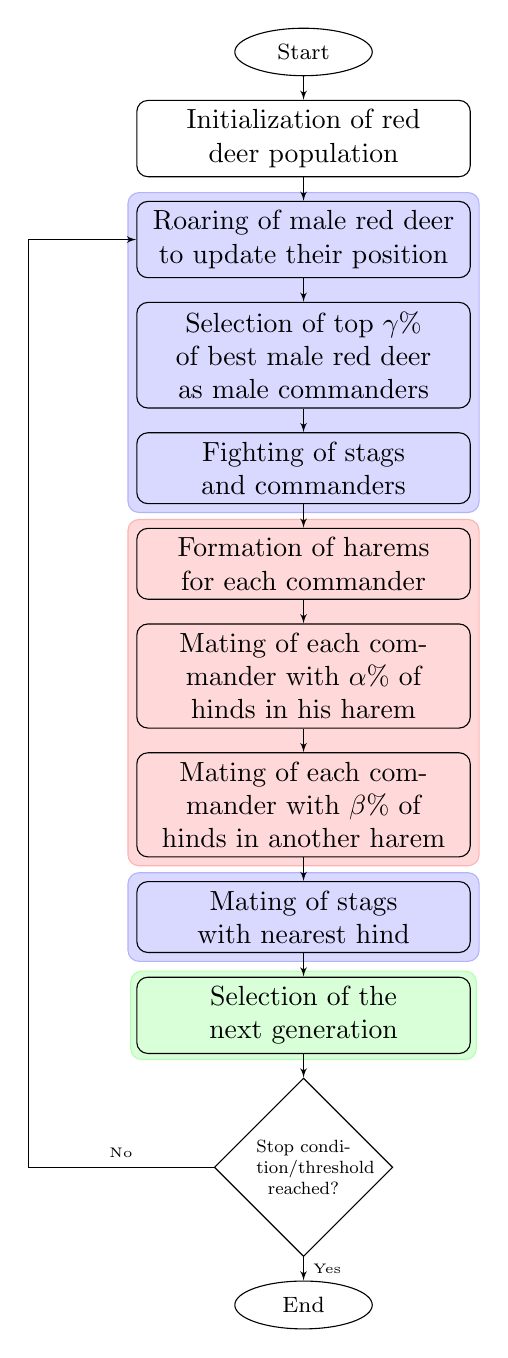
\begin{tikzpicture}[
      node distance = 0.5cm,
      auto,
      block/.style={rectangle, draw, rounded corners, text width=4cm, text centered, minimum height=0.6cm}, 
      ellipse_block/.style={ellipse, draw, text width=1cm, text centered, minimum height=0.6cm, font=\footnotesize},
      decision/.style={diamond, draw, text width=1.5cm, text centered, minimum height=0.6cm, font=\footnotesize},
      line/.style={draw, -latex', very thin},
      blue_block/.style={block, fill=blue!15},
      red_block/.style={block, fill=red!15},
      green_block/.style={block, fill=green!15}
  ]
  
  \node [ellipse_block] (start) {Start};
  \node [block, below=0.3cm of start] (init) {Initialization of red deer population};
  \node [blue_block, below=0.3cm of init] (roar) {Roaring of male red deer to update their position};
  \node [blue_block, below=0.3cm of roar] (select) {Selection of top $\gamma$\% of best male red deer as male commanders};
  \node [blue_block, below=0.3cm of select] (fight) {Fighting of stags and commanders};
  \node [red_block, below=0.3cm of fight] (harem) {Formation of harems for each commander};
  \node [red_block, below=0.3cm of harem] (mate1) {Mating of each commander with $\alpha$\% of hinds in his harem};
  \node [red_block, below=0.3cm of mate1] (mate2) {Mating of each commander with $\beta$\% of hinds in another harem};
  \node [blue_block, below=0.3cm of mate2] (mate3) {Mating of stags with nearest hind};
  \node [green_block, below=0.3cm of mate3] (next) {Selection of the next generation};
  \node [decision, below=0.3cm of next, scale=0.8] (stop) {Stop condition/threshold reached?};
  \node [ellipse_block, below=0.3cm of stop] (end) {End};

  \path [line] (start) -- (init);
  \path [line] (init) -- (roar);
  \path [line] (roar) -- (select);
  \path [line] (select) -- (fight);
  \path [line] (fight) -- (harem);
  \path [line] (harem) -- (mate1);
  \path [line] (mate1) -- (mate2);
  \path [line] (mate2) -- (mate3);
  \path [line] (mate3) -- (next);
  \path [line] (next) -- (stop);
  \path [line] (stop) -- node[right, font=\tiny] {Yes} (end);
  \path [line] (stop) -| node[near start, above, font=\tiny] {No} ++(-3.5,0) |- (roar);

  \begin{scope}[on background layer]
    \node[fit=(roar)(select)(fight), fill=blue!15, rounded corners, draw=blue!30, inner sep=3pt] {};
    \node[fit=(harem)(mate1)(mate2), fill=red!15, rounded corners, draw=red!30, inner sep=3pt] {};
    \node[fit=(mate3), fill=blue!15, rounded corners, draw=blue!30, inner sep=3pt] {};
    \node[fit=(next), fill=green!15, rounded corners, draw=green!30, inner sep=2pt] {};
  \end{scope}
  
  \end{tikzpicture}
  \caption{Flowchart for workflow of red deer algorithm \cite{red_deer}}
  \label{fig:rda-flowchart}
\end{figure}

A closely related approach by Venkata Srinivas et al. \cite{VenkataSrinivas2023_RDA} leveraged the Red Deer Algorithm for cloud task scheduling. However, that work primarily focused on a single objective fitness function and did not perform a comparative evaluation with other algorithms. Our proposed RDA model extends beyond this by introducing a multi objective Qos(Quality of Service) aware fitness function and performing  statistical validation by analyzing multiple experiments across various scenarios against four established metaheuristic algorithms.

\singlespacing \noindent The main contributions of this work are summarized as follows:

\begin{itemize}
\item An RDA-based cloud task scheduling approach is proposed for heterogeneous cloud environments.
\item A multi-objective QoS-aware fitness function is designed to optimize makespan, response time, execution cost, resource utilization, and load balancing simultaneously.
\item The proposed model is evaluated under heterogeneous VM configurations and varying workload scales using CloudSim Plus.
\item Extensive experimental analysis including convergence analysis, parameter sensitivity analysis, scalability analysis, robustness evaluation, and statistical validation is performed.
\item The proposed approach is bench-marked against multiple metaheuristic scheduling algorithms including GA, PSO, GWO, and WOA.
\end{itemize}

The remainder of this paper is organized as follows: Section \ref{sec2} discusses related work in the domain. Section \ref{sec3} presents the proposed model. The development of the RDA in accordance with the proposed model is detailed in Section \ref{sec4}. Section \ref{sec5} outlines the experimental setup, while Section \ref{sec6} presents the results and analysis. Finally, Section \ref{sec7} concludes the paper with future research directions.

\FloatBarrier
\section{Related Work}\label{sec2}

Goyal and Singh \cite{AntColonyOptimization} used Ant based Load Balancing Algorithm (ALBA) but with a neat twist, that is, rather than treating pheromones in their usual way they linked them directly to resources. Resources that handle tasks successfully get rewarded with more pheromone while failures reduce pheromones. It over time pushes tasks towards less busy resources. They performed their tests on GridSim under two different setups. First, they kept the resources fixed and varied the number of tasks, then they kept the number of tasks fixed while varying resources. The results look promising at first. Resource usage is much more balanced with minimal spread but there are concerns that need discussion. Firstly, it has only been compared against a basic baseline of WALBA but no attempt has been made to compare it against alternates like PSO, GA, or even other variants of ACO which makes it hard to judge its competitiveness. Additionally the scale of test bed is too small. Paper only explores load distribution while other metrics such as makespan, response time, energy usage, or fault tolerance are not discussed hence it difficult to tell how it would perform in practical cloud environments.

Kruekaew and Kimpan \cite{bib12} introduced Heuristic Task Scheduling with Artificial
Bee Colony (HABC) algorithm which combines swarm intelligence with scheduling algorithms like FCFS, SJF and LJF with an aim to improve VM scheduling and get better load distribution in the the cloud. They conducted their experiments on CloudSim across twelve different datasets among which some are random while others follow a normal or skewed distribution. Results look good on paper,  HABC with LJF reduces makespan values and also reduces load imbalance. VM processing time variation is smaller compared to ACO, PSO and even improved PSO which suggests an evenly distributed workload. There are several limitations that come up if we look a bit closer. The authors themselves admit that only a limited number of datasets were used and real cloud environments are unpredictable. So naturally question the arises whether these results would hold at scale and in practical scenarios. There are other limitations too. Task dependencies are not considered and scheduling decisions are driven by job length, this simplification that does not always reflect practical workflows. Reliability, fault tolerance, energy usage, or cost efficiency and other important metrics are not discussed. The algorithm’s performance depends on parameter settings hence it is not entirely plug and play. While the results are promising, they may not hold when conditions change.

Sefati et al. \cite{GWO} used Grey Wolf Optimization (GWO) for the problem of load balancing in the cloud. This algorithm takes inspiration from the social hierarchy and hunting behavior of grey wolf packs. Node with the most neighboring nodes is chosen as the cluster head followed by wolf agents that explore the solution space and assign each VM a load threshold . VMs that have a value greater than this threshold are marked as overloaded and all the remaining VMs are evaluated based on a fitness function that combines QoS and load balancing. Reliability for each VM is calculated influenced by failure rate and task weight after which the best candidate solutions guide the final VM selection. Benchmarked in CloudSim against ABC, PSO, and GA, GWO achieved the best results in terms of makespan, response time and operational cost. However, there are several limitations that question the practical relevance of the work. The authors themselves acknowledge that the testbed is too small and eighty tasks across a single three host data center fails to capture real world cloud deployments. QoS dimensions like fault tolerance or scalability are not evaluated but are identified by the authors for future work. The GWO configuration is fixed with no sensitivity analysis reported raising concerns about how the results would hold across varying workloads and cloud configurations.

Anbarkhan and Rakrouki \cite{PSO} introduced Enhanced PSO (EPSO) to improve PSO’s tendency to converge into suboptimal solutions in cloud scheduling. Three modifications drive this approach. First a preprocessing step where tasks are classified into two categories, computationally intensive or IO intensive and merges related subtasks into independent units, this reduces the dimensionality before the search starts. Second, an initialization strategy that assigns the top 25\% most data heavy tasks to best performing resources while randomly assigning the rest. Third, a fitness function that is defined as reciprocal of makespan, simple and direct aimed purely to minimize completion time. Evaluated in CloudSim, EPSO completed 300 task workflows in 255.145 seconds against 394.156 (HPSO) and 459.562 (PSO). Independent scheduling told the same story. 225.523 seconds for EPSO against 254.246 (HPSO) and 327.789 (PSO), for 100 task workflow, the algorithm converged after approximately 25 iterations. Good numbers. But there are real concerns that should not be overlooked.  A single node with 300 task ceiling is a sheltered environment and such setups tend to flatter the algorithms running inside them. The initial split of 25/75 is fixed. No mechanism to adjust when resource availability changes mid execution. The fitness function only optimizes for makespan ignoring other metrics like load balance, VM utilization, fault tolerance which the authors identify as future improvements. Classification of tasks into compute intensive or IO intensive tasks is a simplification that doesn’t translate to real workflows. Finally, comparing only against standard PSO and HPSO two variants of same algorithm does not say much about EPSO’s competitiveness.

Lilhore et al. \cite{lilhore2025} introduced a hybrid algorithm that combines Water Wave Optimization (WWO) and ACO for load balancing and resource allocation. Architecture is clean, ACO provides local exploitation while WWO provides global exploration. The two algorithms do not run in parallel ACO goes first and these solutions then seed WWO phase. Best solutions from both are combined via a Pareto dominance framework targeting four objectives at the same time i.e. response time, resource consumption, operational cost, and energy consumption. When evaluated in CloudSim against GA, WWO, ACO, and Spider Monkey Optimization. The hybrid approach reduced scheduling time and energy consumption while maintaining a balanced workload distribution. Results make a strong case for this approach. But there are real concerns that should not be overlooked and are flagged by the authors themselves. The algorithm is computationally expensive since it runs two metaheuristic algorithms one after the other. Parameter tuning may be necessary based on the implementation environment. Future work tackling computational scalability, task dependency, and real deployment validation would strengthen its practical impact.


\singlespacing \noindent A brief comparison of the above-discussed related work is presented in Table~\ref{tab:relatedwork}.


\begin{table}[htbp]
\caption{Comparison of related load balancing algorithms in cloud computing}
\label{tab:relatedwork}
\begin{tabular*}{\textwidth}{@{\extracolsep\fill}p{2.5cm}p{2cm}p{3cm}p{3cm}}
\toprule
\textbf{Author(s)} & \textbf{Algorithm} & \textbf{Advantages} & \textbf{Limitations} 
\\
\midrule
Goyal and Singh \cite{AntColonyOptimization} & ALBA & More uniform resource utilization in grid environments & Grid-specific, only compared against a no-load-balancing baseline
\\
\\
Kruekaew and Kimpan \cite{bib12} & HABC, ABC & Minimizes makespan; improves load balance & Needs parameter tuning; high operational cost 
\\
\\
Sefati et al. \cite{GWO} & GWO & Lower response time and cost; considers reliability & Computational overhead; lacks security/scalability
\\
\\
Anbarkhan and Rakrouki \cite{PSO} & EPSO & Reduces particle dimensionality via workflow task preprocessing, improved initialization ensures higher initial solution quality, achieves lower makespan and cost compared to PSO and HPSO & Limited to small-scale workloads (max 300 tasks), single-objective fitness function ignores load balancing, energy, and fault tolerance; narrow comparative evaluation against only two baselines 
\\
\\
Lilhore et al. \cite{lilhore2025} & Hybrid WWO-ACO & 
Reduced task scheduling time, lower energy consumption, 
improved resource utilization, and superior load balancing 
across homogeneous and heterogeneous cloud environments & 
High computational overhead, performance variability across 
different cloud infrastructures
\\
\botrule
\end{tabular*}
\end{table}
\begin{figure}[htbp]
\centering
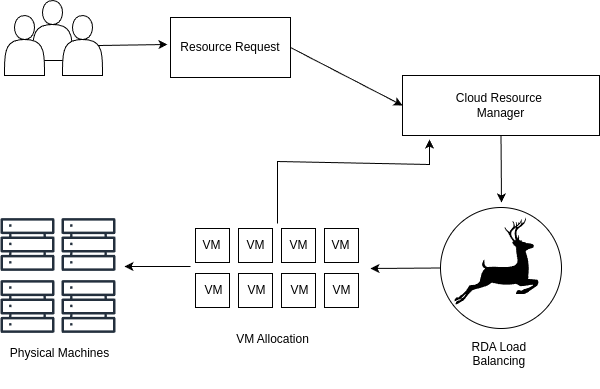
\includegraphics[width=0.9\textwidth]{Images/RDA/proposed-load-balancing-system.png}
\caption{The proposed load-balancing system}\label{LoadBalancing}
\end{figure}


\FloatBarrier
\section{Proposed Model}\label{sec3}

In cloud computing, vast networks of data centers and users are spread globally. 
When numerous user requests flood the cloud simultaneously, efficient organization 
and service delivery are essential. The cloud must distribute workloads evenly 
across resources to ensure fairness. Load balancing remains a key challenge, 
requiring equal distribution of tasks to maintain user satisfaction. Various 
load-balancing algorithms exist for distributed, grid, and cloud systems 
\cite{JinchengLoadBalancing}. While metaheuristic approaches such as GA, GWO, 
PSO, and WOA have been applied to cloud scheduling, RDA a nature-inspired metaheuristic modeled on the mating and 
territorial behavior of Scottish red deer not previously 
been investigated for cloud load balancing. RDA's biologically inspired 
exploration exploitation mechanism, which combines competitive fighting, harem 
formation, and multi-level mating strategies, offers a structurally distinct 
search dynamic compared to existing metaheuristic schedulers. This structural 
novelty motivates its application to the cloud scheduling problem, where 
balancing multiple competing QoS objectives under heterogeneous resource 
conditions remains an open challenge. This study therefore proposes the first 
RDA based load balancing approach for cloud environments, 
incorporating a multi-objective QoS aware fitness function that simultaneously 
optimizes response time, execution cost, resource utilization, and workload 
distribution during task scheduling. The proposed load balancing system is shown in Fig.~\ref{LoadBalancing} and is discussed in Section ~\ref{subsec3.1}.


\subsection{Problem Statement}\label{subsec3.1}
Consider a cloud $C$ consisting of $N$ physical machines, which can be mathematically represented using Eq. (\ref{Eq1}).
\begin{equation}
C = \{PM_1, PM_2,\ldots,PM_N\}
\label{Eq1}
\end{equation}
Additionally, each physical machine consists of multiple VMs, which can be mathematically represented using Eq. (\ref{Eq2}).
\begin{equation}
PM_i = \{VM_{i1}, VM_{i2},\ldots,VM_{iM}\}
\label{Eq2}
\end{equation}

In Eq. (\ref{Eq2}), $VM_{i1}$ and $VM_{iM}$ represent the first and last virtual machines, respectively corresponding to $i^{th}$  physcial machine. Our aim is to minimize costs and maximize the utilization of resources by evenly distributing workload across all the VMs. Efficient load balancing is the key to our approach; otherwise, the system would waste unnecessary time and energy on its tasks. To tackle this, our study proposes an efficient, multi-objective load-balancing approach using the RDA algorithm.

Our model treats the resource allocation as a multi-objective optimization problem and seeks to:
\begin{enumerate}
    \item Minimize the makespan time to enhance task completion time and efficiency,
    \item Maximize utilization of resources to improve infrastructure efficiency,
    \item Minimize costs to make it economically viable,
    \item Reduce response time to maintain QoS.
\end{enumerate}

These objectives tend to be conflicting with one another, and they need to be balanced properly. For example, aggressively reducing makespan may raise the demand for provisioning more resources, which can raise costs and lower overall utilization \cite{GWO}. Hence, the model employs a weighted approach towards red deer, and these objectives allow system administrators to assign weights based on their intended use of the VMs. This helps in maintaining the overall system performance under evolving requirements.

Consistent with the majority of metaheuristic cloud scheduling studies discussed in Section~\ref{sec2}, the proposed model assumes that cloudlets are independent, with no inter task data or precedence dependencies, and that the cloud environment (VM availability, capacity, and cost) remains static over the scheduling horizon, i.e., VM failure and recovery events and dynamically arriving workloads are not modeled. These assumptions isolate scheduling-objective performance from confounding system level effects and are revisited as limitations in Section~\ref{sec7}.

\subsection{Parameters of QoS}\label{subsec3.2}

Makespan, utilization of resources, response time, and cost-effectiveness are performance measures that, collectively, constitute a holistic framework for quantifying the effectiveness of resource allocation policies \cite{bib12}. The model introduced here attempts to promote resource allocation in cloud environments by balancing these performance measures.

The proposed model considers heterogeneous virtual machines with varying computational capacities, execution costs, and availability levels to better simulate realistic cloud computing environments.

\subsubsection{Makespan}\label{subsubsec3.2.1}
Makespan time represents the total time required to complete the scheduled tasks \cite{GWO}. In our model, we are considering the maximum makespan time among all VMs, it is mathematically represented as Eq. (\ref{makespan_eq}).

\begin{equation} \label{makespan_eq}
\text{Makespan} = \max\{CT_1, CT_2, \dots, CT_M\}
\end{equation}% Figure number displayed separately as in original

where CT\textsubscript{i} represents the completion time of $i^{th}$ virtual machine, and M is the total number of available VMs. Our goal is to reduce makespan time to guarantee timely execution of tasks.

\subsubsection{Resource Utilization}\label{subsubsec3.2.2}
Resource utilization is the ratio of time a VM is actively processing tasks to the makespan time \cite{GWO}. Resource utilization for an individual VM, which can be mathematically represented using Eq. (\ref{utilization_for_each_vm_eq})

\begin{equation} \label{utilization_for_each_vm_eq}
\text{Utilization}_{VM_j} = \frac{\sum_{i=1}^{n} PT_{ij}}{\text{Makespan}}
\end{equation}

where \( PT_{ij} \) represents the processing time of the $i^{th}$ task which was processed on \(j^{th} VM\). The total resource utilization across the cloud is then determined by Eq.(\ref{overall_resource_utilization_eq})

\begin{equation} \label{overall_resource_utilization_eq}
\text{Resource Utilization} = \frac{\sum_{j=1}^{m} \text{Utilization}_{VM_j}}{m}
\end{equation}

This metric provides information on how effectively available computational resources are being used in the present situation. Increased utilization ratios indicate better resource management, which can reduce the operational expenses as well as the environmental impact.

\subsubsection{Response Time (RT)}\label{subsubsec3.2.3}

 We model the response time in our model by utilizing space shared basis queuing behavior of tasks on Vms. Space shared is a resource allocation policy where each cloudlet uses a single core at a time, and the remaining wait in a queue until other resources become available to be utilized \cite{space-shared}.

The response time is defined as the time that a cloudlet takes from the time of arrival to its completion time. 

The execution time for cloudlet $C_i$ on the virtual machine $v_j$ can be mathematically represented as Eq (\ref{ResponseTime_for_each_vm_eq}).

\begin{equation} \label{ResponseTime_for_each_vm_eq}
RT_{exec}(C_i, v_j) = \frac{Len}{MIPS_j}
\end{equation}

where $Len$ is the cloudlet length in Million Instructions (MI), and $MIPS_j$ is the processing speed of virtual machine $v_j$.

Since the space shared policy allows limited concurrent execution on a VM, cloudlets assigned to the same VM may experience queuing delays before execution. Therefore, the response time $RT(C_i)$ includes both waiting time and execution time during task scheduling. The average response time is modeled mathematically as Eq. (\ref{Avg_response_time_eq}).

\begin{equation} \label{Avg_response_time_eq}
RT_{avg} = \frac{1}{n} \sum_{i=1}^{n} (FT_i - AT_i)
\end{equation}

where \(FT_i\) and \(AT_i\) represent the finish time and arrival time of cloudlet \(i\), respectively. Lower values of the response time indicate better scheduling and faster execution.

\subsubsection{Cost}\label{subsubsec3.2.4}

The cost model incorporates both resource consumption and temporal factors \cite{GWO}. For a set of \( k \) VMs assigned to user requests, the total cost is expressed mathematically as Eq. (\ref{cost_eq}).

\begin{equation} \label{cost_eq}
\text{Cost} = \sum_{i=1}^{k} C_i \cdot T_i
\end{equation}

where \( C_i \) represents the execution cost rate of \( VM_i \), and \( T_i \) denotes the total execution time of tasks assigned to that VM. The overall cost increases with longer execution durations and higher resource consumption. Minimizing this parameter helps improve the economic efficiency of cloud resource allocation.

\subsection{Fitness Function}\label{subsec3.3}
All the QoS parameters use different units, Some parameters (e.g., utilization) have a positive contribution to fitness, while others (e.g., response time, cost, makespan) have a negative impact \cite{GWO}. Hence, they need to be normalised on a single scale to measure the objective function.

Eqs. (\ref{normalise_min}) and (\ref{normalise_max}) represent the normalization formula for the minimizing and maximizing parameters, respectively \cite{normalise-HB-cloud-paper}.

\begin{equation} \label{normalise_min}
N_{Q^i} =
\begin{cases}
\frac{Q^i - Q^i_{\min}}
{Q^i_{\max} - Q^i_{\min}},
& Q^i_{\max} \neq Q^i_{\min} \\
0, & \text{otherwise}
\end{cases}
\end{equation}

\begin{equation} \label{normalise_max}
N_{Q^i} =
\begin{cases}
\frac{Q^i_{\max} - Q^i}
{Q^i_{\max} - Q^i_{\min}},
& Q^i_{\max} \neq Q^i_{\min} \\
1, & \text{otherwise}
\end{cases}
\end{equation}

For minimization objectives such as makespan, response time, and execution cost, lower normalized values indicate better scheduling quality. In contrast, for maximization objectives such as resource utilization, higher normalized values represent better performance.
The fitness function is given as Algorithm \ref{alg:fitness_function}.

\begin{algorithm}
\small
\caption{Fitness Function}\label{alg:fitness_function}
\begin{algorithmic}[1]
\Procedure{EvaluateFitness}{$solution$}
    \State Initialize $cost$, $responseTime$, and VM processing statistics
    \State Retrieve VM parameters including MIPS, execution cost, and availability
    
    \For{each $cloudlet_i$ in $solution$}
        \State Decode $solution_i$ to obtain assigned $VM_j$
        \State Calculate execution time of $cloudlet_i$ on $VM_j$
        \State Update VM processing time and scheduling metrics
    \EndFor
    
    \State Calculate $makespan$ using Eq. (\ref{makespan_eq}), $avgUtilization$ using Eqs. (\ref{utilization_for_each_vm_eq}) and (\ref{overall_resource_utilization_eq}), $avgResponseTime$ using Eqs. (\ref{ResponseTime_for_each_vm_eq}) and (\ref{Avg_response_time_eq}), $totalCost$ using Eq. (\ref{cost_eq})
    \State Normalize all QoS metrics
    \State Compute final fitness value using the weighted sum model Eq. (\ref{fitness})
\EndProcedure
\end{algorithmic}
\end{algorithm}

To effectively balance the QoS parameters during resource allocation, a unified fitness function is designed which evaluates each candidate solution based on normalized QoS metrics, ensuring correctness regardless of their original scales \cite{GWO}. 

\singlespacing \noindent The overall fitness \( F \) of a solution is computed as Eq. (\ref{fitness}).

\begin{equation} \label{fitness}
Fitness = w_1 \cdot N_{makespan} + w_2 \cdot N_{utilization} + w_3 \cdot N_{cost} + w_4 \cdot N_{RT}
\end{equation}

where $N_{makespan}$, $N_{utilization}$, $N_{RT}$, and $N_{cost}$ are the normalized parameters of makespan, utilization, response time and cost, respectively, and $w_1$ to $w_4$ are user-defined weights satisfying $\sum w_i = 1$. Optimizing solely one parameter could lead to resource under utilization. Hence, By assigning appropriate weights, users could emphasize on specific objectives based on their operational context.

The weights assigned to each QoS parameter in the fitness function Eq. (\ref{fitness}) are shown in Table~\ref{tab:weights}. Makespan and Response Time are given higher importance to achieve more efficient task completion and reduced latency, while utilization and cost are also considered for balanced resource allocation.

\begin{table}[htbp]
\centering
\caption{Weight values used in the fitness function}
\label{tab:weights}
\begin{tabular}{|c|c|c|}
\hline
\textbf{Weight} & \textbf{Parameter} & \textbf{Value} \\ \hline
$w_1$ & Makespan & 0.30 \\ \hline
$w_2$ & Resource Utilization & 0.25 \\ \hline
$w_3$ & Cost & 0.20 \\ \hline
$w_4$ & Response Time & 0.25 \\ \hline
\end{tabular}
\end{table}

The proposed RDA technique for load balancing in cloud computing is presented in Algorithm~\ref{alg:rda_load_balancing}. The algorithm describes the initialization, population update, mating strategies, and fitness-based VM allocation process employed to optimize resource utilization, minimize makespan, reduce response time, and control execution cost within the cloud environment, which is discussed further in Section \ref{sec4}.

%  RDA Algo ==============
\begin{algorithm}
\small
\caption{RDA for Load Balancing in Cloud Computing}\label{alg:rda_load_balancing}
\begin{algorithmic}[1]
\Procedure{RedDeerAlgorithm}{$numVMs, numCloudlets $}
    \State \textbf{Initialize:} $populationSize, numMales, numHinds, \alpha, \beta, \gamma, UB,$
    \State \hspace{10em} $LB, maxIterations$

    \State $numCommanders \gets \lfloor \gamma \times numMales \rfloor$
    \State $numStags \gets numMales - numCommanders$
    \State $bestFitness \gets \infty$

    \State \textbf{Initialize Population:} Generate $populationSize$ random cloudlet-to-VM mapping solutions
    \ForAll{deer $d$ in $population$}
        \State $d.fitness \gets$ \Call{\ref{alg:fitness_function} EvaluateFitness}{$d.position$}
    \EndFor

    \State Sort population in ascending order of fitness
    \State $males \gets$ top $numMales$ individuals
    \State $hinds \gets$ remaining individuals
    \State $commanders \gets$ top $numCommanders$ from $males$
    \State $stags \gets$ remaining $males$

    \For{$iter = 1$ to $maxIterations$}
        \Comment{Roaring Phase}
        \ForAll{$male$ in $males$}
            \State Update $male$ position if fitness improves via roaring
        \EndFor

        \State Sort $males$ by fitness
        \State Update $commanders$ and $stags$

        \Comment{Fighting Phase}
        \ForAll{$commander$ in $commanders$}
            \State Select random $stag$
            \State Generate new positions by fighting
            \State Update $commander$ with best position
        \EndFor

        \Comment{Harem Formation}
        \State Calculate relative fitness of commanders for harem allocation
        \State Divide $hinds$ into harems proportional to fitness

        \Comment{Mating Phase}
        \ForAll{$commander$ in $commanders$}
            \State Mate with a proportion $\alpha\%$ of hinds in the same harem
            \State Mate with a proportion $\beta\%$ of hinds from another harem
        \EndFor

        \ForAll{$stag$ in $stags$}
            \State Find nearest hind and mate
        \EndFor

        \Comment{Selection Phase}
        \State Select the best individuals for the next population using tournament selection
        \State Update $bestPosition$ and $bestFitness$ if improved
        \State Break if convergence criteria are satisfied
    \EndFor

    \State \Return Mapping of cloudlets to VMs using $bestPosition$
\EndProcedure
\end{algorithmic}
\end{algorithm}

In Fig. \ref{fig:representation_of_red_deer} of the proposed model, each candidate solution represents a cloudlet-to-VM mapping vector, where each index corresponds to a cloudlet and the stored value indicates the VM assigned for its execution. The scheduling objective is to identify an optimal mapping that balances workload distribution while satisfying multiple QoS requirements.

\FloatBarrier
\section{Development of the RDA According to the Proposed Model}\label{sec4}
In the proposed approach, the primary objective is to support real-time cloud applications, where adherence to task deadlines is critical. Each task is associated with a user-defined execution time constraint, and the system endeavors to complete the execution of the task within the specified time frame to uphold QoS requirements.

The RDA is a nature-inspired metaheuristic technique modeled after the mating behavior of Scottish red deer during the breeding season. In the context of cloud computing, this algorithm is adapted to solve the resource allocation problem, specifically mapping cloudlets to virtual machines by simulating the social dynamics of the red deer. Each individual red deer represents a candidate solution encoding a potential mapping of cloudlets to VMs as illustrated in Fig. ~\ref{fig:representation_of_red_deer}. The algorithm outputs the optimal mapping of cloudlets to VMs that balances multiple objectives: makespan, resource utilization, cost efficiency, and response time.

\subsection{Generation of Initial Red Deer Population}\label{subsec4.1}

A population of $N_{\text{pop}} = 100$ red deer is initialized, where each red deer represents a feasible cloudlet-to-VM mapping solution. Each red deer is encoded as a one-dimensional array of size equal to the number of cloudlets, denoted as $N_c$, where each element stores the identifier of the VM assigned to the corresponding cloudlet. Mathematically, this representation can be expressed as Eq.~(\ref{representation_of_a_red_deer_as_a_cloudlet_to_VM_eq})

\begin{equation}\label{representation_of_a_red_deer_as_a_cloudlet_to_VM_eq}
RD_i = [x_1, x_2, x_3, \dots, x_{N_c}]
\end{equation}

where $RD_i$ denotes the $i$-th red deer, and $x_j \in \{1, 2, \ldots, N_{\text{vm}}\}$ represents the VM identifier assigned to the $j$-th cloudlet, with $N_{\text{vm}}$ being the total number of available VMs.
 
Fig. ~\ref{fig:representation_of_red_deer} illustrates the population representation structure. Each row corresponds to one red deer (candidate solution), while each column represents a cloudlet. The value at position $(i, j)$ denotes the VM identifier assigned to cloudlet $j$ in solution $RD_i$. For example, if $x_1 = 4$, then cloudlet 1 is allocated to virtual machine 4 for execution.

\begin{figure}[htbp]
\centering
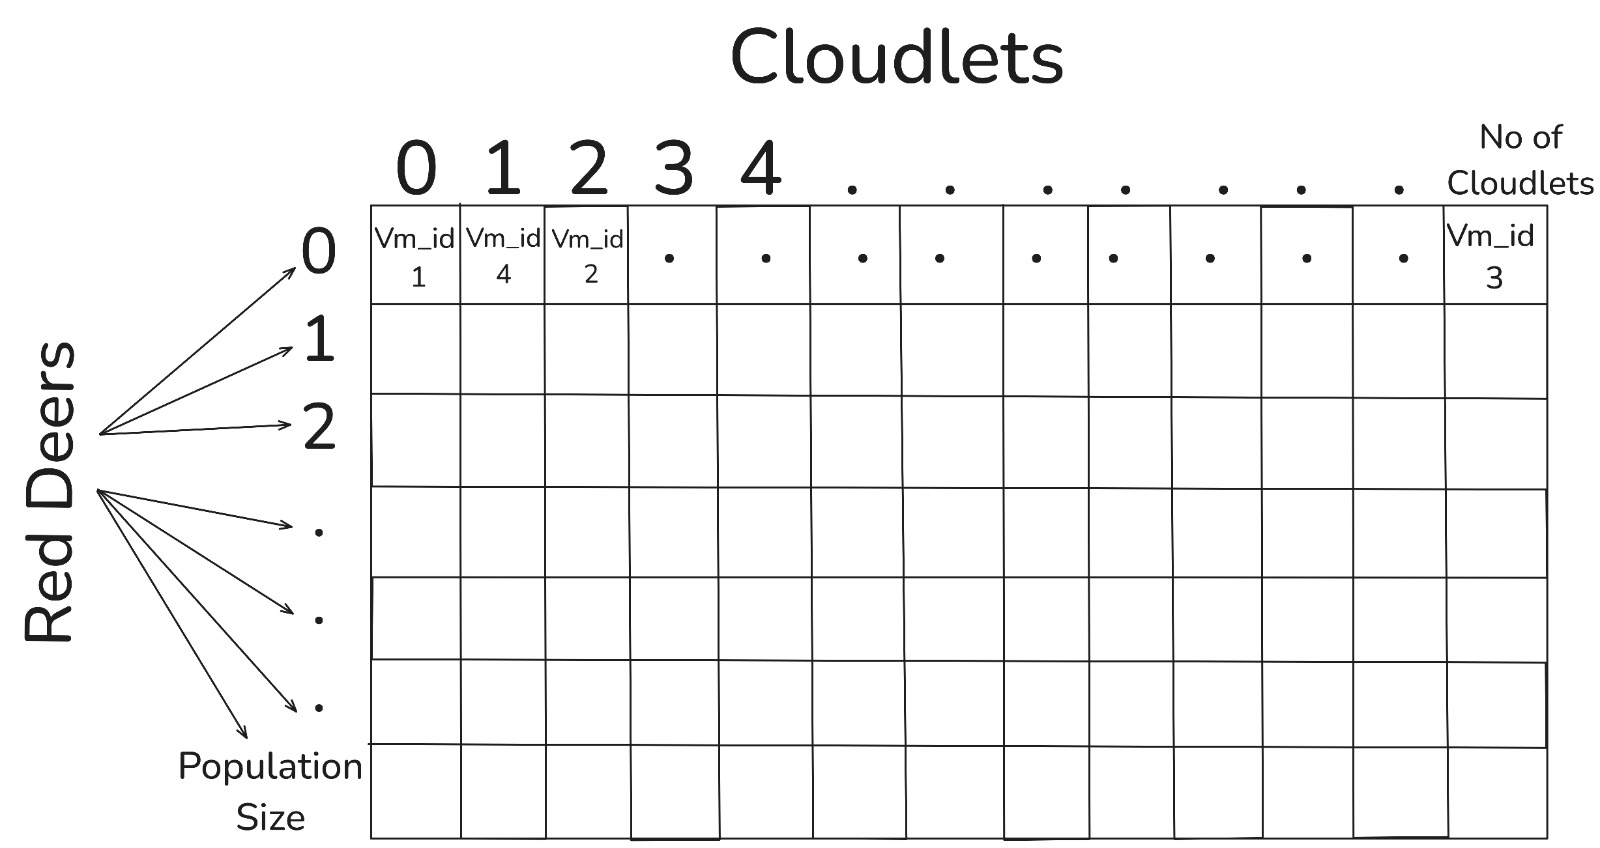
\includegraphics[width=0.9\textwidth]{Images/RDA/representation_of_a_red_deer_as_a_cloudlet_to_VM.jpeg}
\caption{Representation of a red deer as a cloudlet-to-VM mapping solution}
\label{fig:representation_of_red_deer}
\end{figure}

After generating the initial population, the fitness of each red deer is evaluated by following Algorithm~\ref{alg:fitness_function} based on makespan, resource utilization, response time, and execution cost using Eq. (\ref{fitness}).

Once fitness values are obtained, the population is sorted in ascending order of fitness (where lower fitness values indicate better solutions). The selection process can be mathematically represented as Eq. (\ref{eq:population_sorting}).
 
\begin{equation}\label{eq:population_sorting}
\text{Sorted} = \{RD_1, RD_2, \ldots, RD_{N_{\text{pop}}} \mid f(RD_i) \leq f(RD_{i+1})\}
\end{equation}
 
Subsequently, the top-performing $N_{\text{male}}$ red deer are selected as males, from which the top $\gamma\%$ are designated as commanders. The remaining male red deer are classified as stags, and the rest of the population comprises hinds. This stratification process can be formalized as Eq. (\ref{male_red_deer_eq}).

\begin{equation}\label{male_red_deer_eq}
M = \{RD_1, RD_2, \dots, RD_{N_{\text{male}}}\}
\end{equation}

The remaining individuals are considered as hinds:

\begin{equation}\label{hinds_eq}
H = \{RD_{N_{\text{male}} + 1}, RD_{N_{\text{male}} + 2}, \dots, RD_{N_{\text{pop}}}\}
\end{equation}

Here, $N_{male}$ as represented in Eq. (\ref{male_red_deer_eq}) controls the intensification capability of the algorithm by preserving high-quality solutions, while the $N_{hind}$ population as illustrated in Eq. (\ref{hinds_eq}) contributes to the diversification and exploration of the search space.

\subsection{Roaring Process}\label{subsec4.2}
In the roaring phase, each male red deer attempts to improve its current solution (i.e., cloudlet-to-VM mapping) by exploring its neighborhood in the solution space. This behavior mimics the natural tendency of red deer to expand their territory and display dominance by roaring.

\begin{figure}[htbp]
\centering
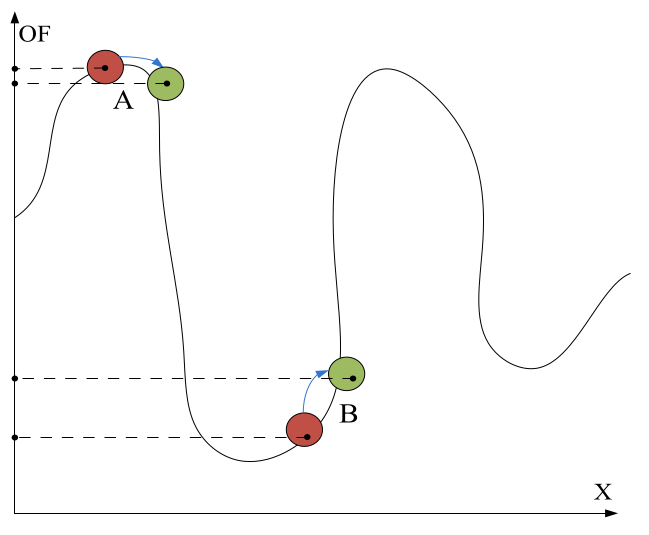
\includegraphics[width=0.9\textwidth]{Images/RDA/roaring_phase_fig.png}
\caption{Roaring process of male red deer \cite{red_deer}}
\label{roaring_figure_ref}   
\end{figure}

To simulate this behavior computationally, each male red deer \( RD_i \in M \) updates its position according to the following rule \cite{red_deer} that can be represented mathematically as Eq. (\ref{roaring_phase_eq}).

\begin{equation}\label{roaring_phase_eq}
male^{\text{new}}_i =
\begin{cases}
male^{\text{old}}_i + a_1 \cdot (((UB - LB) \cdot a_2) + LB), & \text{if } a_3 \geq 0.5 \\
male^{\text{old}}_i - a_1 \cdot (((UB - LB) \cdot a_2) + LB), & \text{if } a_3 < 0.5
\end{cases}
\end{equation}
      
where:
\begin{itemize}
    \item \( male^{\text{old}}_i \) is the current red deer position (i.e., current cloudlet-to-VM assignment),
    \item \( male^{\text{new}}_i \) is the updated solution after roaring,
    \item \( UB = N_{VM} \) and \( LB = 0 \), which denotes the upper and lower bounds of the solution space, respectively. All the numbers in this range represent unique \texttt{vm\_id}s,
    \item \( a_1, a_2, a_3 \in [0, 1] \) are uniformly distributed random numbers.
\end{itemize}

Each male RD generates a new position using the above update rule. The updated solution is accepted only if it yields a better fitness value compared to the previous one. This ensures that the exploration during roaring leads to quality improvements in the mapping.

Fig. \ref{roaring_figure_ref} illustrates two scenarios chosen from the solution space to show the effect of roaring in isolation. Observe that cases A and B normally happen within the roaring period. In case A, the new position is accepted because its objective function value Eq. (\ref{fitness}) is lower than that of the old position. In case B, the new solution is not acceptable. Observe again that the y-axis is the objective function value, and the x-axis is the positions of males in this figure.

\subsection{Selection of the best male red deer as commanders}\label{subsec4.3}
In nature, not all male red deer possess the same level of strength, dominance, or attractiveness. Some exhibit superior traits and are more successful in claiming and defending territories. This variation is modeled in the RDA by classifying male red deer into two distinct groups: \textit{commanders} and \textit{stags} \cite{red_deer}.

In our cloudlet-to-VM mapping scenario, each male red deer represents a potentially optimal mapping configuration. To further intensify the search, we designate the top $\gamma$\% of male red deer (based on fitness value) as commanders and the remaining as stags.

The number of commanders \( N_{\text{Com}} \) is computed using the following formula which is mathematically modeled as Eq. (\ref{Equation:selection_of_commanders}).

\begin{equation}\label{Equation:selection_of_commanders}
N_{\text{Com}} = \text{round}( \gamma \cdot N_{\text{male}} )
\end{equation}

\noindent where:
\begin{itemize}
    \item \( \gamma \in [0, 1] \) is a user-defined parameter representing the percentage of elite males to be chosen as commanders,
    \item \( N_{\text{male}} \) is the total number of male red deer.
\end{itemize}

After selecting the commanders, the remaining male red deer are assigned the role of stags. The number of stags \( N_{\text{stag}} \) is calculated using Eq. (\ref{num_stag_eq}).

\begin{equation}
\label{num_stag_eq}
N_{\text{stag}} = N_{\text{male}} - N_{\text{Com}}
\end{equation}

This division of roles creates a hierarchy among male red deer, which is later used in the fighting and mating phases \cite{red_deer}. In our implementation, we set \( \gamma = 0.45 \), which means that 45\% of male red deer are chosen as commanders which was giving the experimentally best outcome.

\subsection{Fight between male commanders and stags}\label{subsec4.4}
Once the male red deer have been divided into commanders and stags, the next step is to simulate the natural behavior of dominance through fights. Each commander is randomly paired with a stag to engage in a competition to improve the population's overall fitness \cite{red_deer}. These confrontations result in the generation of new candidate solutions through exploitation of the solution space.


\begin{figure}[htbp]
\centering
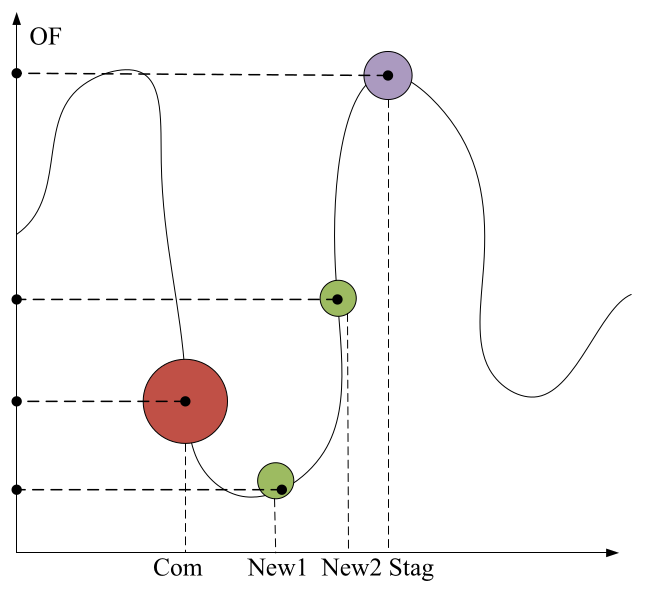
\includegraphics[width=0.9\textwidth]{Images/RDA/fighting_phase_fig.png}
\caption{Fight between a commander and a stag \cite{red_deer}}
\label{fig:fighting_phase}
\end{figure}

For each such pairing, two new solutions are generated using Eqs. (\ref{fighting_eq_1}) and (\ref{fighting_eq_2}) that are represented as:

\begin{equation}\label{fighting_eq_1}
\text{New}_1 = \frac{(\text{Com} + \text{Stag})}{2} + b_1 \cdot ((\text{UB} - \text{LB}) \cdot b_2 + \text{LB})
\end{equation}

\begin{equation}\label{fighting_eq_2}
\text{New}_2 = \frac{(\text{Com} + \text{Stag})}{2} - b_1 \cdot ((\text{UB} - \text{LB}) \cdot b_2 + \text{LB})
\end{equation}

\noindent where:
\begin{itemize}
    \item \( \text{Com} \) and \( \text{Stag} \) denotes the current position vectors (solutions - Cloudlet to VMs mapping) of the commander and stag, respectively,
    \item \( b_1 \) and \( b_2 \) are random variables drawn from a uniform distribution over the interval [0, 1].
\end{itemize}

The commander is replaced with the best solution after evaluating their objective function using Eq. (\ref{fitness}) out of all the four possible solutions as shown in Fig. \ref{fig:fighting_phase} i.e. commander, stag, and the two new offspring using Eqs. (\ref{fighting_eq_1}) and (\ref{fighting_eq_2}) \cite{red_deer}.

\subsection{Form harems}\label{subsec4.5}
In nature, each male commander claims a group of hinds, forming a harem as shown in Fig. \ref{harem_formation_fig_ref} based on his strength and dominance. In our solution, this behavior is simulated by associating a portion of the hind population with each commander based on their fitness values. A lower fitness value indicates a better scheduling solution and therefore results in a larger harem allocation.

\begin{figure}[htbp]
\centering
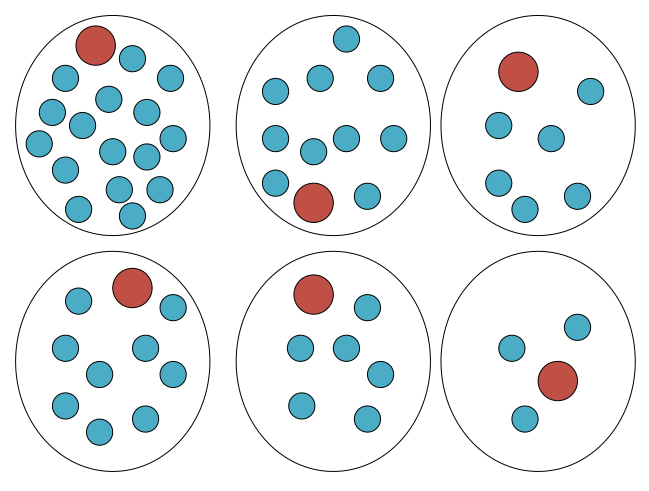
\includegraphics[width=0.9\textwidth]{Images/RDA/harem_formation_fig.png}
\caption{Harems of each commander \cite{red_deer}}
\label{harem_formation_fig_ref}
\end{figure}

Calculate the relative power \( V_n \) of each commander using Eq. (\ref{Equation:relative_power_of_commanders}).

\begin{equation}
\label{Equation:relative_power_of_commanders}
V_n = v_n - \max\{v_i\}
\end{equation}

\noindent where:
\begin{itemize}
    \item \( v_n \) is the fitness value (objective function value) of the \( n \)-th commander,
    \item \( \max\{v_i\} \) represents the worst (here, maximum) fitness among all commanders, ensuring normalization by fitness proximity to optimality.
\end{itemize}

Then, we normalize this value to determine the portion of hinds to be assigned to each commander using Eq. (\ref{normalised_of_each_commander}).

\begin{equation}\label{normalised_of_each_commander}
P_n = \frac{V_n}{\sum_{i=1}^{N_{Com}} V_i}
\end{equation}

\noindent where:
\begin{itemize}
    \item \( P_n \) is the normalized power of the \( n \)-th commander,
    \item \( N_{Com} \) denotes the total number of commanders.
\end{itemize}

Now, based on this proportional power, the number of hinds allocated to the \( n \)-th commander’s harem is computed as Eq. (\ref{harem_formation_eq}).

\begin{equation}\label{harem_formation_eq}
N.{\text{harem}_n} = \text{round}(P_n \cdot N_{\text{hind}})
\end{equation}

\noindent where:
\begin{itemize}
    \item \( N.{\text{harem}_n} \) is the number of hinds of the \( n \)-th commander's harem,
    \item \( N_{\text{hind}} \) is the total number of hinds in the population.
\end{itemize}

The hinds are then randomly assigned to the commanders based on the calculated values \( N.{\text{harem}_n} \). Each selected group of hinds, together with its corresponding commander, constitutes one harem.

\subsection{Mating of commanders with hinds in his harem}\label{subsec4.6}
Like other species in nature, red deer mates with each other. Here, the commander mates with $\alpha$\% of the hinds of his harem and generates offspring. It is calculated using Eq. (\ref{Equation:N_hinds_to_mate_with_commander}).

\begin{equation}\label{Equation:N_hinds_to_mate_with_commander}
N.{\text{Harem}_n^{mate}} = \text{round}(\alpha \cdot N.{\text{Harem}_n})
\end{equation}

\noindent where:
\begin{itemize}
    \item $N.{\text{Harem}_n^{mate}}$ is the number of hinds from the $n$-th harem that will mate with the commander,
    \item $N.{\text{Harem}_n}$ is the total number of hinds in that harem,
    \item $\alpha$ is a user-defined uniform model parameter that controls the mating percentage which is set between 0 and 1 including.
\end{itemize}

Once the hinds for mating are selected randomly from each harem, a new offspring (solution) is produced using the following mathematically modeled Eq. (\ref{offspring_eq})

\begin{equation}\label{offspring_eq}
\text{offs} = \frac{\text{Com} + \text{Hind}}{2} + c \cdot (UB - LB)
\end{equation}\label{offspring}

\noindent where:
\begin{itemize}
    \item $\text{Com}$ and $\text{Hind}$ represent the current position vectors (solutions - Cloudlet to VMs mapping) of the commander and a selected hind,
    \item $\text{offs}$ is the new offspring (i.e., the new candidate solution),
    \item $c$ is a random number generated from a uniform distribution over the interval [0, 1].
\end{itemize}


\subsection{Mating of commander with hinds of another harem}\label{subsec4.7}
Allow each commander to mate with $\beta$\% of hinds from another randomly selected harem \cite{red_deer}. 

Let $i$ be the index of a randomly selected harem which is not itself. The number of hinds in the $i$-th harem that mate with the current commander is given by Eq. (\ref{Equation:N_hinds_to_mate_with_other_commander}).

\begin{equation}\label{Equation:N_hinds_to_mate_with_other_commander}
N.{\text{Harem}_i^{mate}} = \text{round}( \beta \cdot N.{\text{Harem}_i} )
\end{equation}

\noindent where:
\begin{itemize}
    \item $N.{\text{Harem}_i^{mate}}$ is the number of hinds from the $i$-th harem that will mate with the commander,
    \item $N.{\text{Harem}_i}$ is the number of hinds in the $i$-th harem,
    \item $\beta$ is a user-defined parameter controlling the proportion of hinds involved in inter-harem mating, range value of this parameter is between zero and one.
\end{itemize}

Each of the $N.{\text{Harem}_i^{mate}}$ hinds selected from the $i$-th harem mates with the current commander using the same offspring generation formula defined in Section \ref{offspring}. 

\subsection{Mating of stag with the nearest hind}\label{subsec4.8}
Unlike commanders, stags do not form harems but still participate in the mating phase. Each stag mates with the nearest hind in the solution space to generate locally improved offspring solutions.

The nearest hind is determined using Euclidean distance in the $J$-dimensional solution space. The distance between a stag and the $i$-th hind is calculated as Eq. (\ref{stag_mating_eq}).

\begin{equation}\label{stag_mating_eq}
d_i = \sqrt{ \sum_{j=1}^{n} (\text{stag}_j - \text{hind}_{i,j})^2 }
\end{equation}

\noindent where:
\begin{itemize}
    \item $d_i$ is the distance between the stag and the $i$-th hind,
    \item $\text{stag}_j$ and $\text{hind}_{i,j}$ represent the $j$-th dimension of the stag and of the $i$-th hind, respectively,
\end{itemize}

After identifying the nearest hind (i.e., the one with the smallest $d_i$), the stag mates with hind using the Eqs. (\ref{Equation:N_hinds_to_mate_with_commander}) and (\ref{offspring_eq}), replacing the commander’s role with that of the stag.


\subsection{Select the next generation}\label{subsec4.9}
The next generation is formed by combining the current solutions and newly generated offspring. 

To achieve this, two selection strategies are used:

\begin{enumerate}
    \item \textbf{Elite Preservation:} High-quality male red deer solutions, including commanders and stags, are preserved to maintain elite scheduling solutions across generations.
    
    \item \textbf{Offspring Selection:} The remainder of the population is filled by selecting individuals from the pool of all hinds and the offspring generated through the mating processes. This selection is performed using the tournament selection method.
\end{enumerate}

\subsection{Stopping condition}\label{subsec4.10}
The optimization process continues until the maximum number of iterations is reached or convergence is observed in the fitness values across consecutive iterations. Based on preliminary experimentation and parameter sensitivity analysis, the iteration count was set to 100 for the reported simulations.

\subsection{Computational Complexity Analysis}
\label{subsec:complexity_analysis}

This subsection analyzes the computational complexity of the proposed
method. Let \(N\) denote the number of
cloudlets, \(M\) the number of available virtual machines, \(P\) the
population size, and \(I\) the maximum number of iterations. Each deer represents one possible
cloudlet scheduling solution of length \(N\). 

For each candidate solution, the algorithm decodes the assignment of all
cloudlets, calculates their execution and waiting time statistics, updates
the processing load of the assigned VMs, and computes makespan, average
response time, resource utilization, and execution cost. Processing all
cloudlets requires \(O(N)\) time, while aggregating the VM level statistics
requires \(O(M)\) time. Therefore, the time complexity of evaluating one
candidate solution is

\begin{equation}
T_{\mathrm{fitness}} = O(N + M).
\label{eq:fitness_complexity}
\end{equation}

During initialization, \(P\) candidate solutions are generated and evaluated.
Hence, the initialization phase has a time complexity of

\begin{equation}
T_{\mathrm{initialization}} = O(P(N + M)).
\label{eq:initialization_complexity}
\end{equation}

In each iteration, the roaring, fighting, harem formation, and mating
operators update the positions of the deer. Since a solution is represented
by an assignment vector of length \(N\), updating the population requires
\(O(PN)\) time. The newly generated offspring and updated individuals must
then be evaluated, resulting in a fitness-evaluation cost of
\(O(P(N+M))\). Population ranking and selection require sorting up to \(P\)
individuals according to their fitness values, which has a complexity of
\(O(P\log P)\). Therefore, the computational cost per iteration is

\begin{equation}
T_{\mathrm{iteration}} =
O\left(PN + P(N+M) + P\log P\right).
\label{eq:iteration_complexity}
\end{equation}

Since the fitness evaluation phase dominates the remaining operations, the
per-iteration complexity can be expressed as

\begin{equation}
T_{\mathrm{iteration}} =
O\left(P(N+M) + P\log P\right).
\label{eq:iteration_complexity_simplified}
\end{equation}

For a maximum of \(I\) iterations, the total time complexity of the proposed
RDA scheduler is

\begin{equation}
T_{\mathrm{RDA}} =
O\left(I\left[P(N+M)+P\log P\right]\right).
\label{eq:rda_total_complexity}
\end{equation}

The space complexity is primarily determined by storing the population of
candidate schedules. Since each of the \(P\) solutions contains \(N\)
cloudlet to VM assignments, the population requires \(O(PN)\) memory.
Additional arrays storing VM processing times, utilization values, and cost
statistics require \(O(M)\) memory. Thus, the overall space complexity is

\begin{equation}
S_{\mathrm{RDA}} = O(PN + M).
\label{eq:rda_space_complexity}
\end{equation}


Fig. \ref{fig:rda-flowchart} and Algorithm \ref{alg:rda_load_balancing} provides a summarized overview of the main steps involved in the RDA. It highlights the initialization, male classification, roaring, fighting, harem formation, mating, and selection processes that collectively guide the search for optimal load balancing in the cloud environment.

\FloatBarrier
\section{Experimental Setup}\label{sec5}

To evaluate the performance of the proposed scheduling approach under controlled and repeatable conditions, CloudSim Plus was used to simulate a virtual cloud computing environment. CloudSim Plus is an open and extensible simulation framework via which cloud computing infrastructures and resource provisioning policies can be simulated and modeled. It was created at the CLOUDS Laboratory, Department of Computer and Software Engineering, University of Melbourne \cite{cloudsim}, it provides a controlled environment to conduct experiments without the need for a real cloud infrastructure. It allowed us to compare the performance of our proposed algorithm with other existing algorithms effectively. Moreover, CloudSim Plus supports customization by enabling developers to extend or replace its core classes, making it suitable for implementing new scheduling or provisioning policies \cite{cloudsim}.

The overall simulation workflow and interaction between datacenters, hosts, virtual machines, brokers, and cloudlets in CloudSim Plus are illustrated in Fig.~\ref{fig:cloudSimPlus_architecture}. The architecture demonstrates how cloudlets are scheduled and executed over virtualized resources within the simulated cloud environment.

\begin{figure}[htbp]
\centering
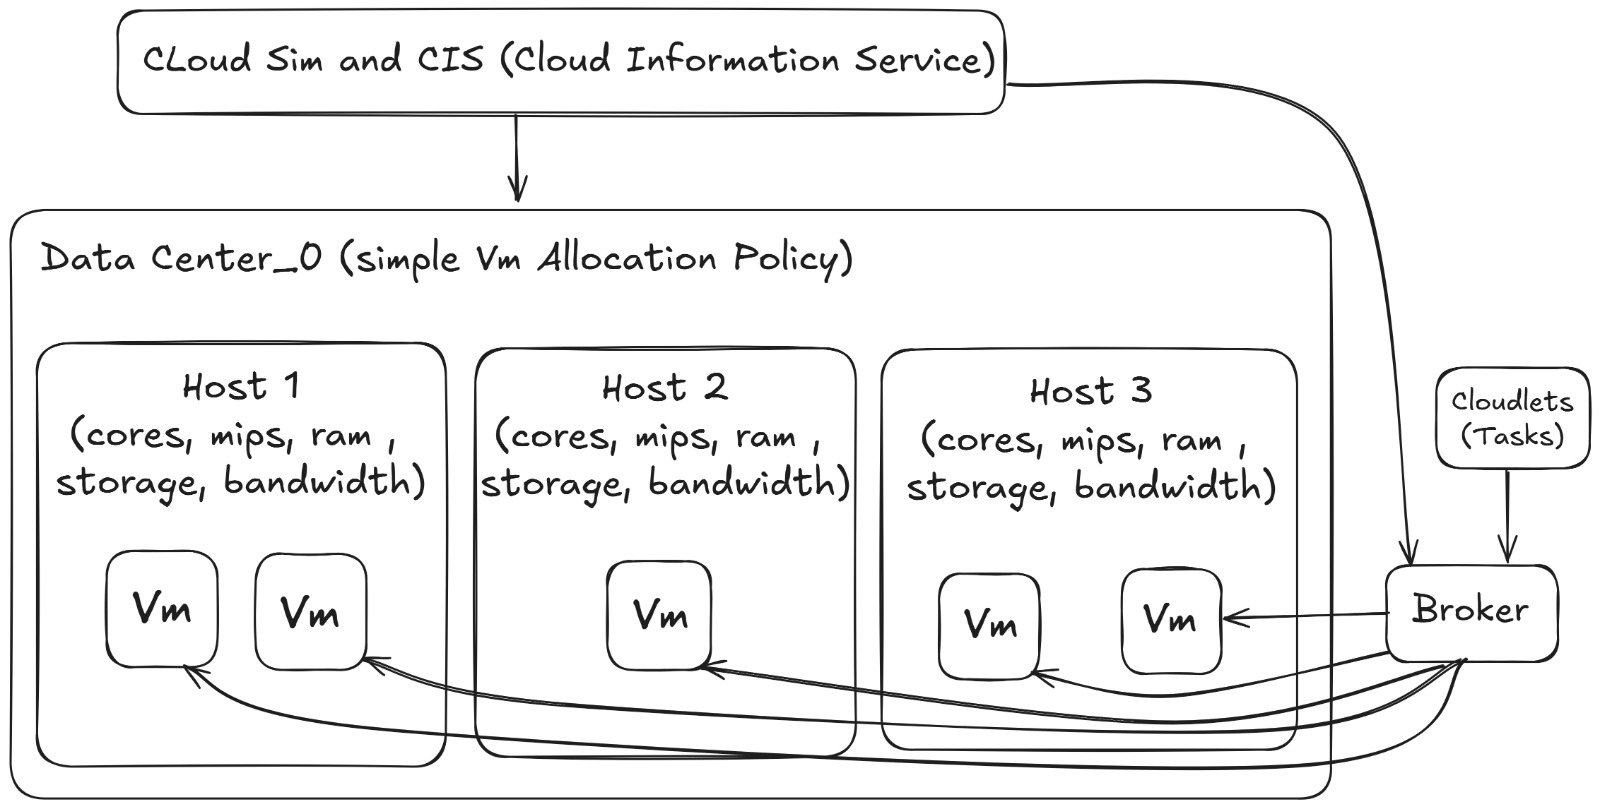
\includegraphics[width=0.9\textwidth]{Images/cloudSimPlus_architecture_fig.jpeg}
\caption{Basic architecture of CloudSim Plus \cite{cloudsimplusPaper}}
\label{fig:cloudSimPlus_architecture}
\end{figure}

\subsection{Simulation Environment Configuration}\label{subsec5.1}
 
The simulation environment has three layers: physical infrastructure, virtual resource allocation, and workload configuration. The following subsections describe each component.
 
\subsubsection{Physical Infrastructure and Virtual Resources}
 
Simulation of multiple hosts and virtual machines with heterogeneous configurations was performed using CloudSim Plus. Table~\ref{tab_hosts} presents the hosts specifications, which are four distinct host types with processing capacities and number of cores ranging from 1,000 to 8,000 MIPS (Million Instructions Per Second) and 1 core to 8 cores respectively. Twenty heterogeneous hosts were simulated while experimenting to evaluate scalability.
 
\begin{table}[htbp]
\centering
\caption{Host specifications used in simulation}\label{tab_hosts}%
\begin{tabular*}{\textwidth}{@{\extracolsep\fill}lcccccc}
\toprule
Host ID & Cores & MIPS & RAM (MB) & Storage (MB) & Bandwidth (Mbps)\\
\midrule
1 & 1 & 1,000 & 51,200 & 1,048,576 & 102,400 \\
2 & 2 & 2,500 & 102,400 & 1,048,576 & 102,400 \\
3 & 4 & 5,000 & 204,800 & 1,048,576 & 102,400 \\
4 & 8 & 8,000 & 204,800 & 1,048,576 & 102,400 \\
\bottomrule
\end{tabular*}
\end{table}
 
The virtual machine configurations are presented in Table~\ref{tab_vm}. Four different VM types were simulated with processing capacities ranging from 1,000 to 4,000 MIPS, memory allocations from 2,048 to 8,192 MB, and availability factor from 0.7 to 1.0. These configurations were selected to represent cloud provider services close real world scenarios. Number of virtual machines simulated for experiments ranged from 10 to 60 machines per experiment.

Space shared scheduling policy was used to ensure sequential cloudlet execution on assigned virtual machines, with full resource utilization assumed during execution.
 
\begin{table}[htbp]
\centering
\caption{Virtual machine types and specifications}\label{tab_vm}
\begin{tabular*}{\textwidth}{@{\extracolsep\fill}lcccc}
\toprule
VM Type & MIPS & RAM (MB) & Cost Rate (\$/hr) & Availability \\
\midrule
VM1 & 1,000 & 2,048 & 0.05 & 1.0 \\
VM2 & 2,000 & 4,096 & 0.08 & 0.9 \\
VM3 & 3,000 & 6,144 & 0.10 & 0.8 \\
VM4 & 4,000 & 8,192 & 0.15 & 0.7 \\
\bottomrule
\end{tabular*}
\end{table}
 
\subsubsection{Workload and Scalability Configuration}
 
Cloudlet workloads ranged from 1,000 to 20,000 Million Instructions (MI), with cloudlet counts varying from 100 to 2,000 per scenario (see Table~\ref{tab_cloudlets}).
 
\begin{table}[htbp]
\centering
\caption{Cloudlet workload configuration}\label{tab_cloudlets}
\begin{tabular*}{\textwidth}{@{\extracolsep\fill}lc}
\toprule
Parameter & Value \\
\midrule
Cloudlet Length & 1,000 - 20,000 MI \\
Number of Cloudlets & 100 - 2,000 \\
Scheduling Policy & Space Shared \\
Utilization Model & Full Utilization \\
\bottomrule
\end{tabular*}
\end{table}
 
Experimental scenarios ranged from small scale configurations (3 hosts, 10 VMs, 100 cloudlets) to large scale configurations (20 hosts, 60 VMs, 2,000 cloudlets) as shown in Table~\ref{tab_scale}.
 
\begin{table}[htbp]
\centering
\caption{Simulation scale configuration}\label{tab_scale}
\begin{tabular*}{\textwidth}{@{\extracolsep\fill}lc}
\toprule
Parameter & Value \\
\midrule
Number of Hosts & 3 - 20 \\
Number of Virtual Machines & 10 - 60 \\
Number of Cloudlets & 100 - 2,000 \\
Host Core Configuration & 4 - 16 cores \\
Host RAM Configuration & 16 GB - 64 GB \\
Scheduling Policy (VM/Cloudlet) & SpaceShared \\
\bottomrule
\end{tabular*}
\end{table}
 
\subsection{Algorithm Configuration and Experimental Parameters}\label{subsec5.2}
 
The RDA parameters were determined through experiments, including sensitivity analysis of different combinations of population size, male to female ratio, and mating behavior coefficients as discussed in Sections \ref{subsec6.3} and \ref{subsec6.4}.

Table~\ref{tab:algo_params} presents the final parameter configuration of RDA and all the other competing algorithms that were used while performing the experiments.

For the Genetic Algorithm (GA), the population size, crossover rate, and mutation rate are set as suggested in the literature \cite{hassanat2019GA, GA}. The parameters of the Grey Wolf Optimizer (GWO) and the Whale Optimization Algorithm (WOA) are set as suggested in their respective original proposed works \cite{mirjalili2014grey, Mirjalili2016WOA}. For the Particle Swarm Optimization (PSO), the base velocity formula and acceleration coefficients ($c_1 = c_2 = 2.0$) have been set as suggested by Kennedy and Eberhart \cite{Kennedy1995}. The inertia weight strategy where $w$ decreases linearly from $0.9$ to $0.4$ over the course of iterations was adopted as proposed by Shi and Eberhart \cite{shi1998modifiedPSO}.

\begin{table}[htbp]
\centering
\caption{Tuned parameters of the metaheuristic algorithms}\label{tab:algo_params}
\begin{tabular}{@{}p{0.28\textwidth}p{0.68\textwidth}@{}}
\toprule
Algorithm & Parameters \\
\midrule
Genetic Algorithm (GA)
  & Initial population $= 100$; maximum number of iterations $= 100$;
    crossover rate $= 0.8$; mutation rate $= 0.01$;
    selection strategy: tournament selection \\[3pt]
Grey Wolf Optimizer (GWO)
  & Initial population $= 100$; maximum number of iterations $= 100$;
    convergence factor $a$ decreases linearly from $2$ to $0$;
    coefficient vectors $\vec{A}$ and $\vec{C}$ computed automatically
    from the iteration count; hierarchy: $\alpha$, $\beta$, $\delta$,
    $\omega$ \\[3pt]
Particle Swarm Optimization (PSO)
  & Swarm size $= 100$; maximum number of iterations $= 100$;
    inertia weight $w$ decreases linearly from $0.9$ to $0.4$; cognitive coefficient $c_1 = 2.0$;
    social coefficient $c_2 = 2.0$; $r_1, r_2 \in [0,1]$
    (uniform random) \\[3pt]
Whale Optimization Algorithm (WOA)
  & Initial population $= 100$; maximum number of iterations $= 100$;
    convergence factor $a$ decreases linearly from $2$ to $0$;
    spiral shape constant $b = 1$;
    switching probability $p \in [0,1]$ (uniform random)
    \\[3pt]
Red Deer Algorithm (RDA)
  & Population size $= 100$; maximum number of iterations $= 100$;
    male population $= 20\%$; commander fraction $\gamma = 0.45$;
    harem mating ratio $\alpha = 0.35$;
    inter-harem mating ratio $\beta = 0.30$;
    solution bounds $= [0.0,\; N_{\text{VM}} - 1]$ \\
\bottomrule
\end{tabular}
\end{table}
 
Solution bounds $N_{\text{VM}}$ in Table \ref{tab:algo_params} for RDA denote the total number of virtual machines available. 
 
\subsection{Performance Evaluation Setup}\label{subsec5.3}
 
All experiments were performed on a Lenovo Yoga 6 laptop (Intel Core i5 13th Gen, 16 GB RAM) using CloudSim Plus as the simulation framework. The proposed RDA approach was compared against four established metaheuristic algorithms: Genetic Algorithm (GA), Particle Swarm Optimization (PSO), Grey Wolf Optimizer (GWO), and Whale Optimization Algorithm (WOA). All algorithms were evaluated under identical simulation configurations, workload scenarios, and performance metrics to ensure fair comparative analysis. 

\FloatBarrier
\section{Results and Analysis}\label{sec6}

\subsection{Makespan Analysis}\label{subsec6.1}

Makespan is the total execution time it takes to execute all the cloudlets on a virtual machine, starting from the submission time of the very first cloudlet to the finish time of the final cloudlet task. It's the primary metric to evaluate RDA's scheduling efficiency and scalability. Fig. ~\ref{fig:makespan_analysis} shows the makespan time for the workload ranging from 100 to 2,000 cloudlets.

\begin{figure}[htbp]
\centering
\begin{subfigure}[t]{0.49\textwidth}
    \centering
    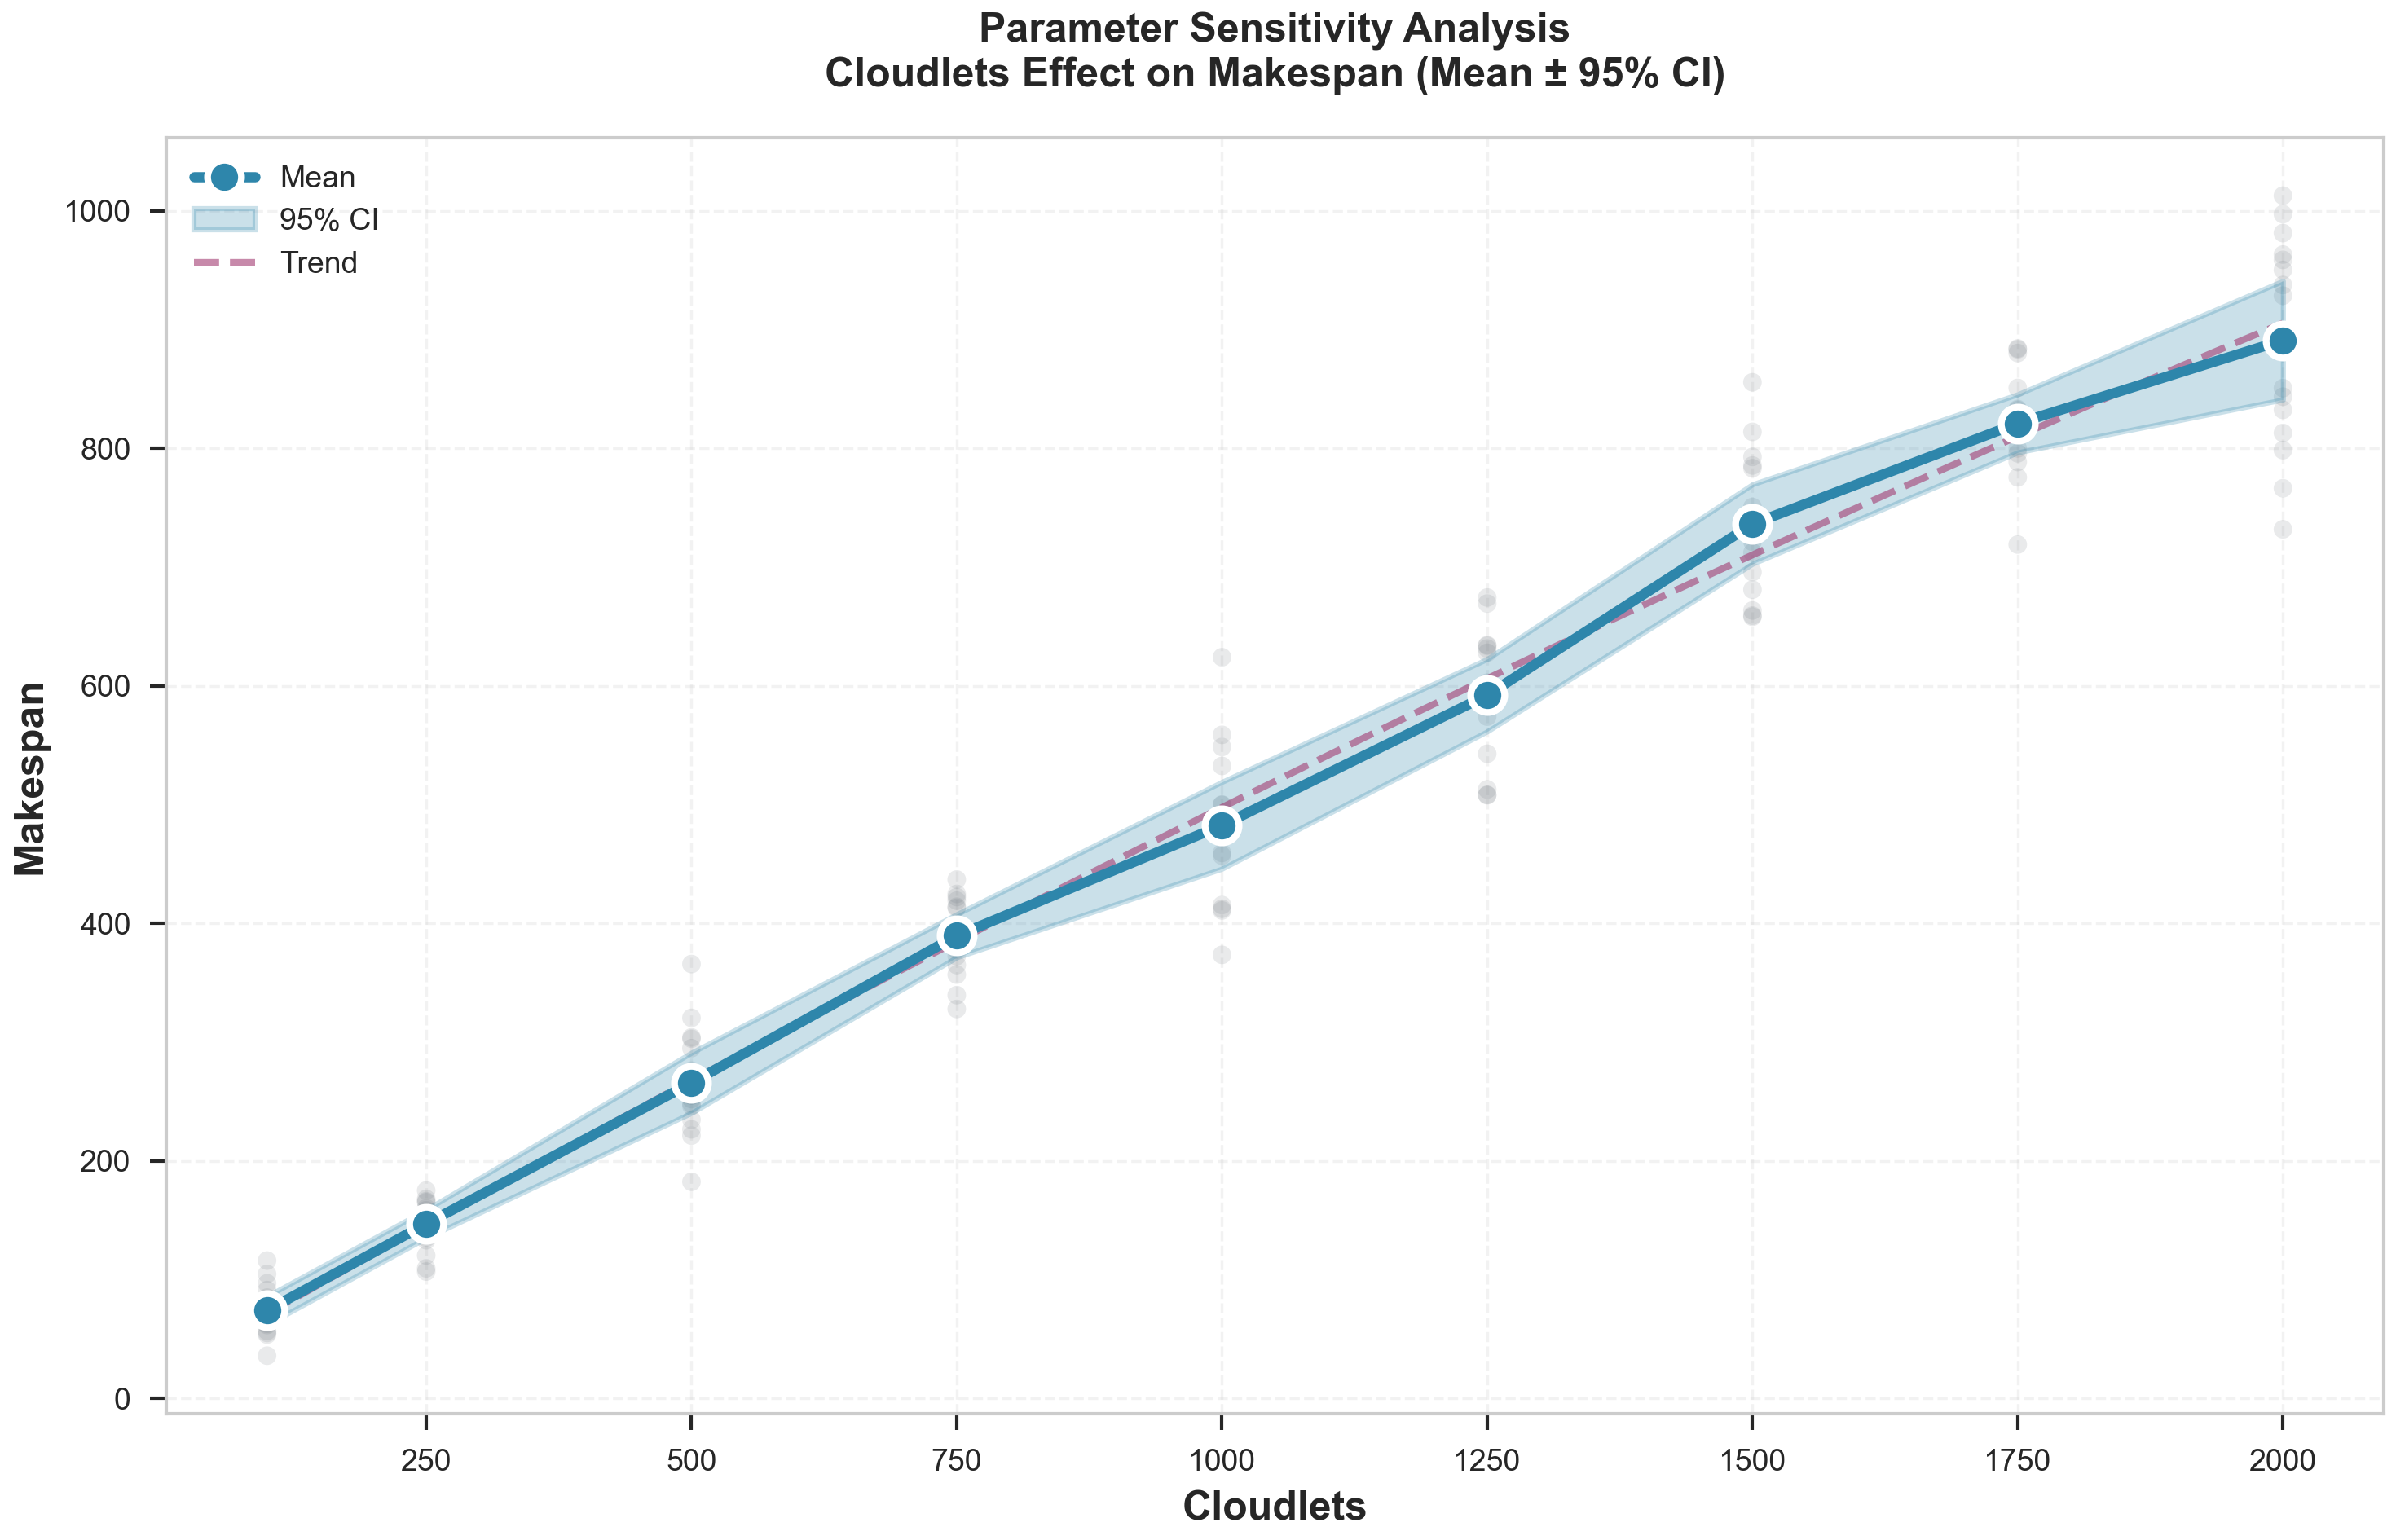
\includegraphics[
        width=\linewidth,
        trim=15 15 15 15,
        clip
    ]{Images/Results/Cloudlets_Makespan.png}
    \caption{Makespan under varying cloudlet workloads}
    \label{fig:cloudlets_makespan}
\end{subfigure}
\hfill
\begin{subfigure}[t]{0.49\textwidth}
    \centering
    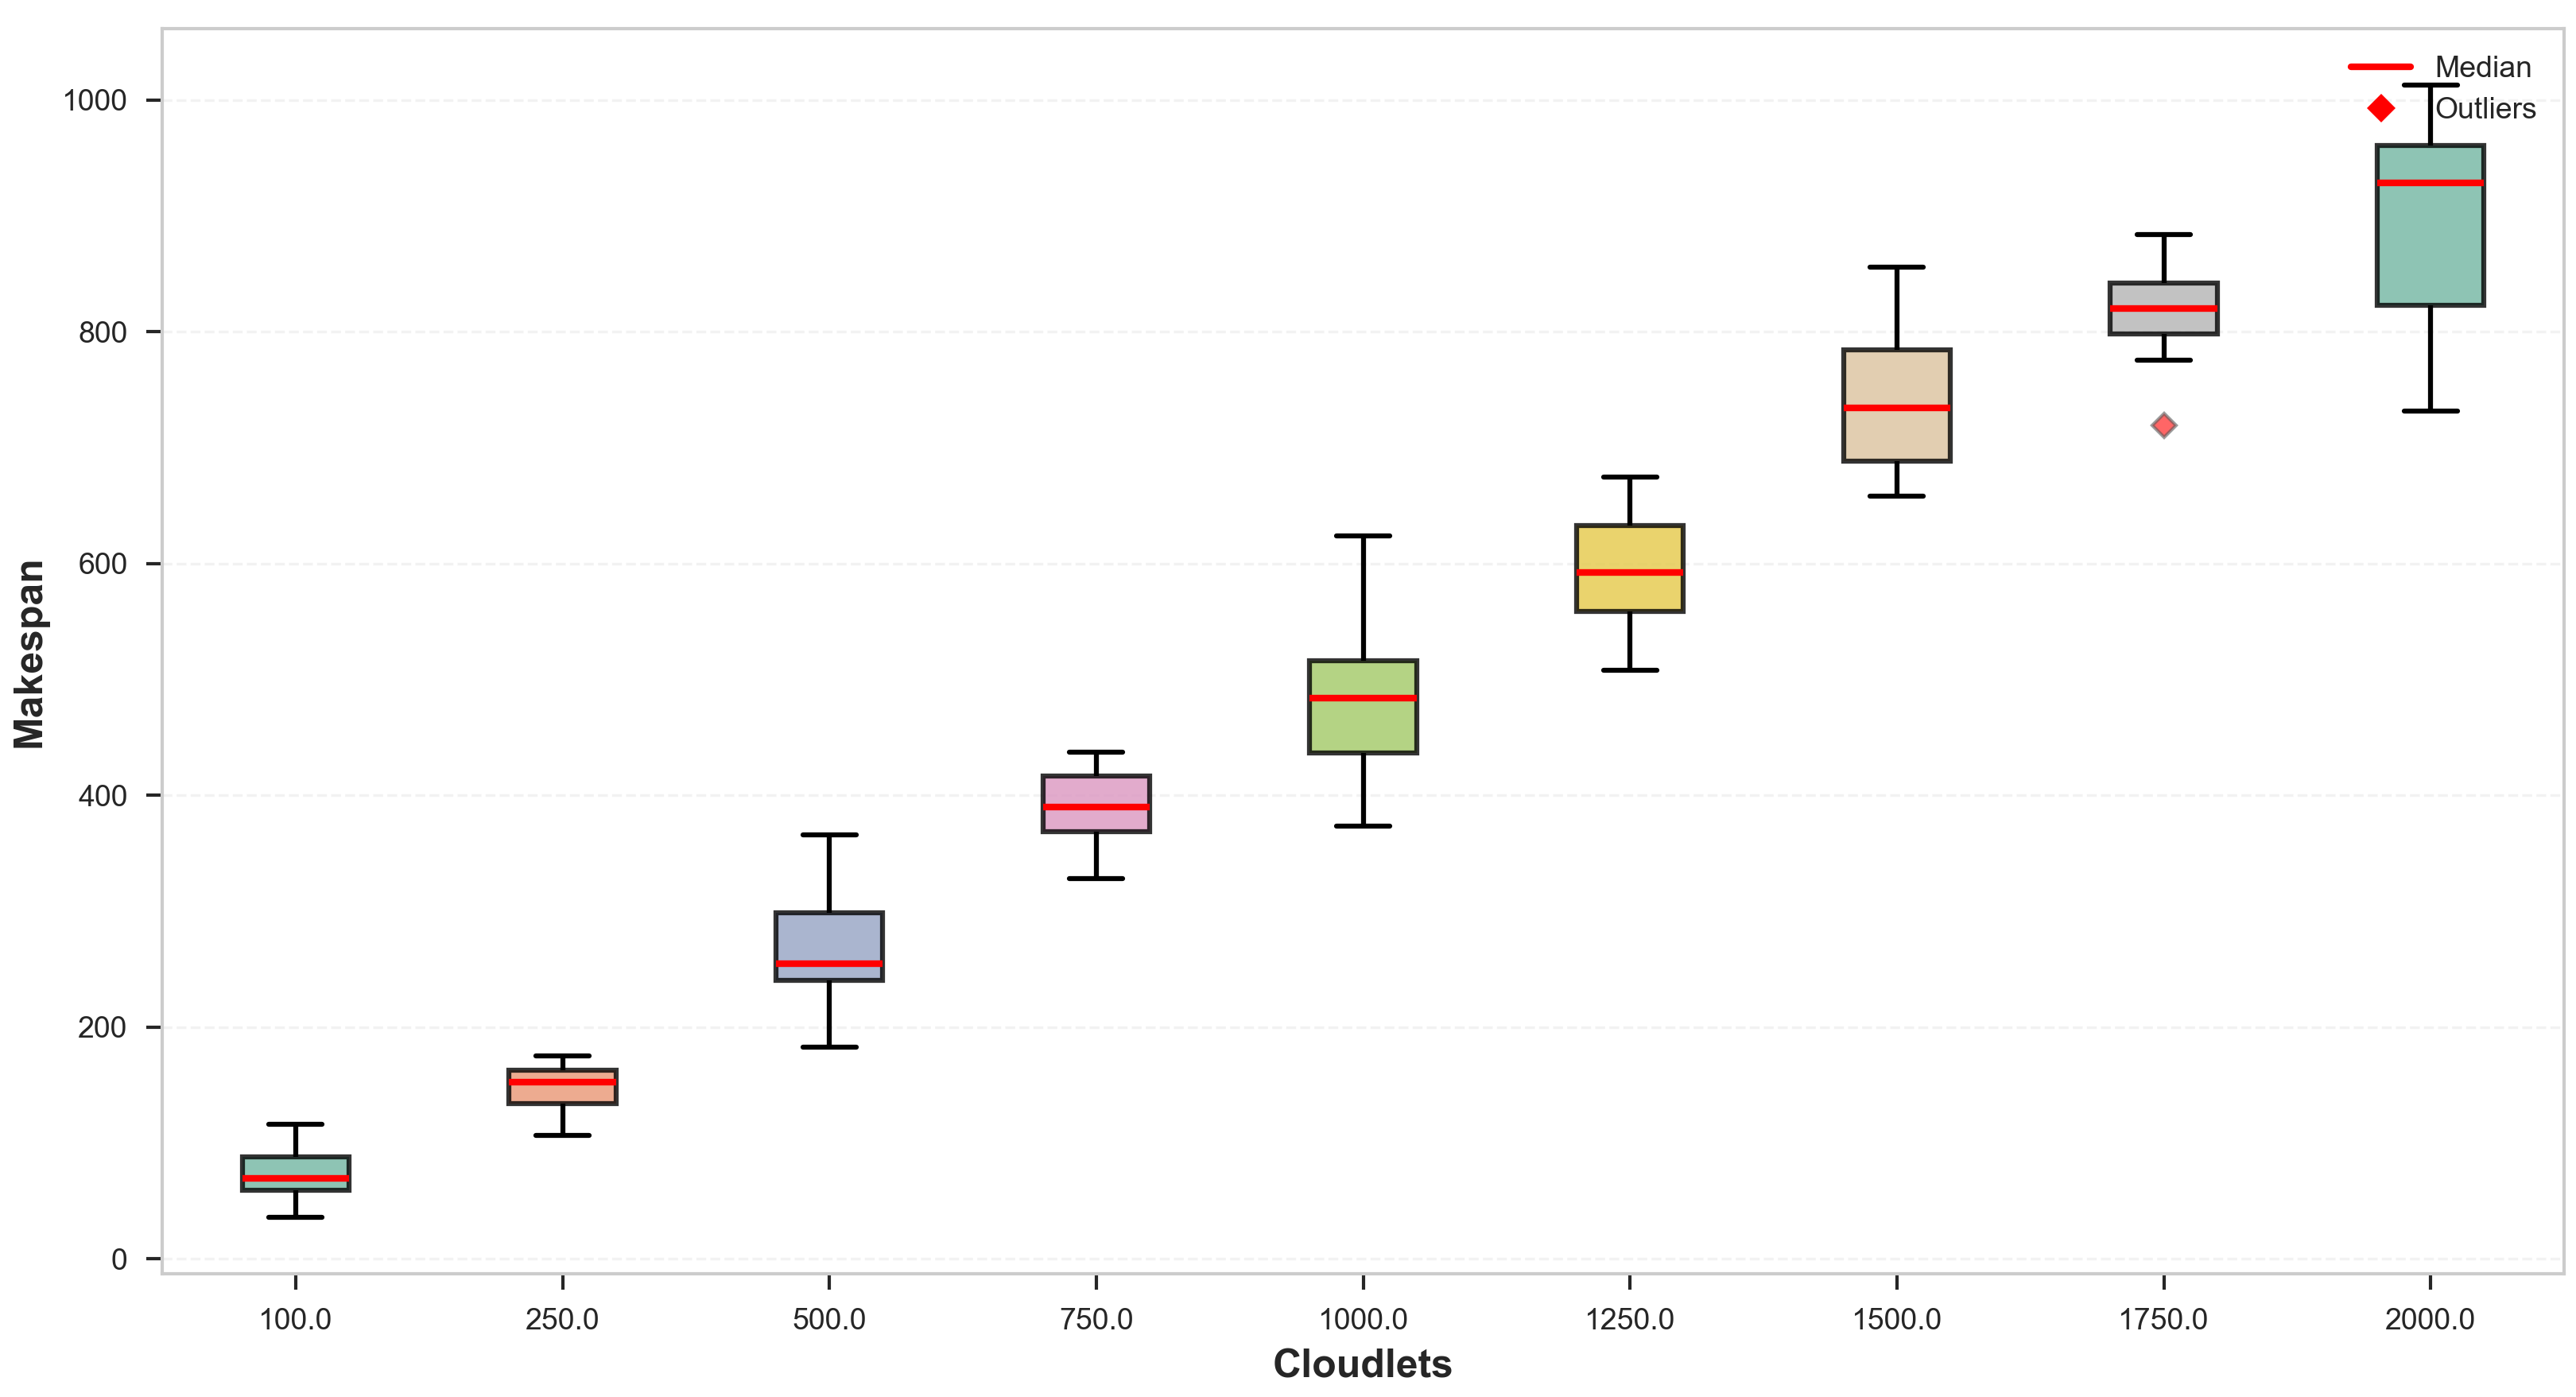
\includegraphics[
        width=\linewidth,
        trim=15 15 15 15,
        clip
    ]{Images/Results/boxplot_Cloudlets_Makespan.png}
    \caption{Box-plot analysis of makespan distribution}
    \label{fig:boxplot_cloudlet_makespan}
\end{subfigure}
\caption{Makespan analysis of the proposed scheduling approach under different workload configurations}
\label{fig:makespan_analysis}
\end{figure}

\textbf{Scaling Behavior:} The RDA model scales makespan linearly with respect to the increase in workload as shown in Fig.  \ref{fig:cloudlets_makespan}. Mean makespan values shows a growth from 78 ms at 100 cloudlets to 890 ms at 2,000 cloudlets, which is an 11.41× increase in makespan for a 20× increase in cloudlet workload. The result shows that the ratio of makespan by workload scales by 0.571, which is a great factor for scalability. 

\textbf{Consistency and Robustness:} Box-plot in Fig. ~\ref{fig:boxplot_cloudlet_makespan} shows that makespan distributions were highly stable across various simulations. 

The inter-quartile range representing the central 50\% of makespan values, remained within 30–50 ms, maintaining a coefficient of variation below 5\%. This consistency is further indicated by the close agreement between mean and median values. At the maximum workload of 2,000 cloudlets, the mean and median differed by only 40 ms (4.5\%), suggesting near‑symmetric behavior without significant outliers.

The absence of outliers and the stability around the median together supports the RDA model's consistent and reliable scheduling performance.

\subsection{Response Time Analysis}\label{subsec6.2}

Response time is the scheduling delay from a cloudlet submission to it's execution initiation. It's a critical QoS metric that impacts service reliability for the user. Fig. ~\ref{fig:response_analysis} represents RDA's response time behavior across varying workloads and the comparative performance of RDA against competing algorithms.

\subsubsection{Scaling Behavior Under Increasing Workload}

The proposed RDA model showed response times increasing steadily from 17 ms at 100 cloudlets to 200 ms at 2,000 cloudlets, with median values tracking closely (17 ms to 198 ms respectively) which is the correct expected growth in a cloud environment. The alignment of mean and median values across the entire workload range indicates symmetric response time distributions.

\begin{figure}[htbp]
\centering
\begin{subfigure}[t]{0.49\textwidth}
    \centering
    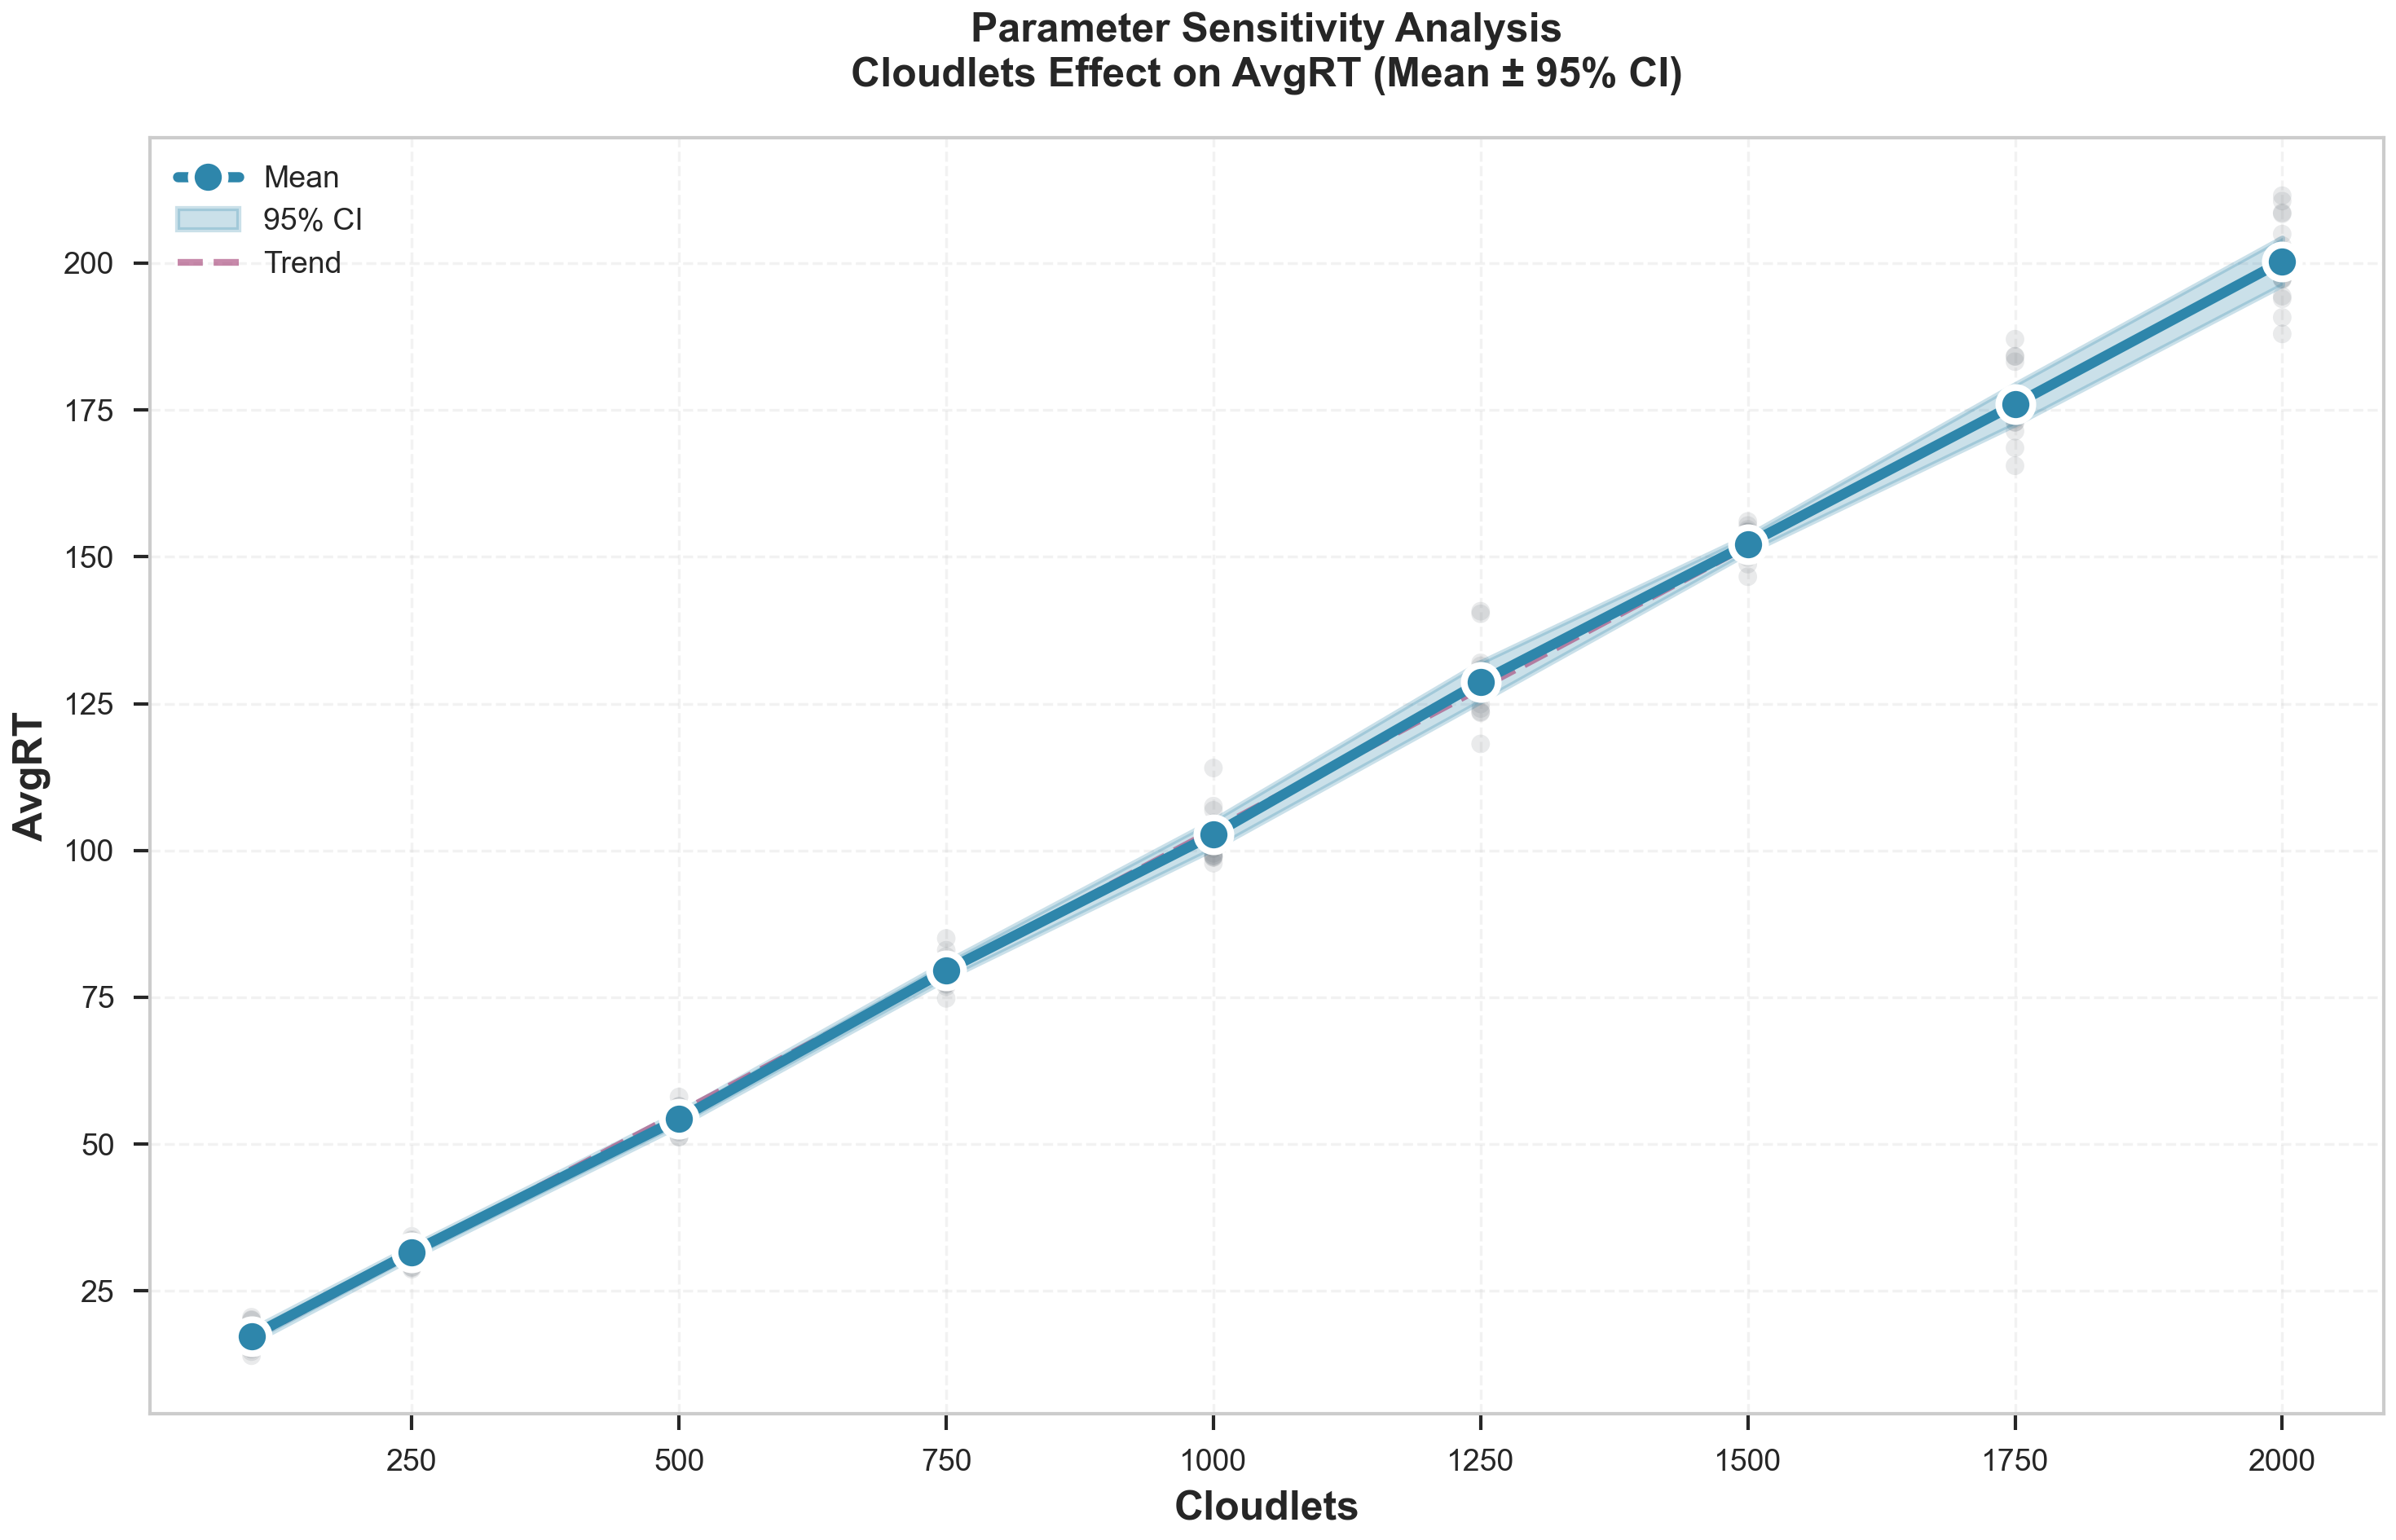
\includegraphics[
        width=\linewidth,
        trim=15 15 15 15,
        clip
    ]{Images/Results/Cloudlets_AvgRT.png}
    \caption{Average response time under varying cloudlet workloads}
    \label{fig:cloudlets_rt}
\end{subfigure}
\hfill
\begin{subfigure}[t]{0.49\textwidth}
    \centering
    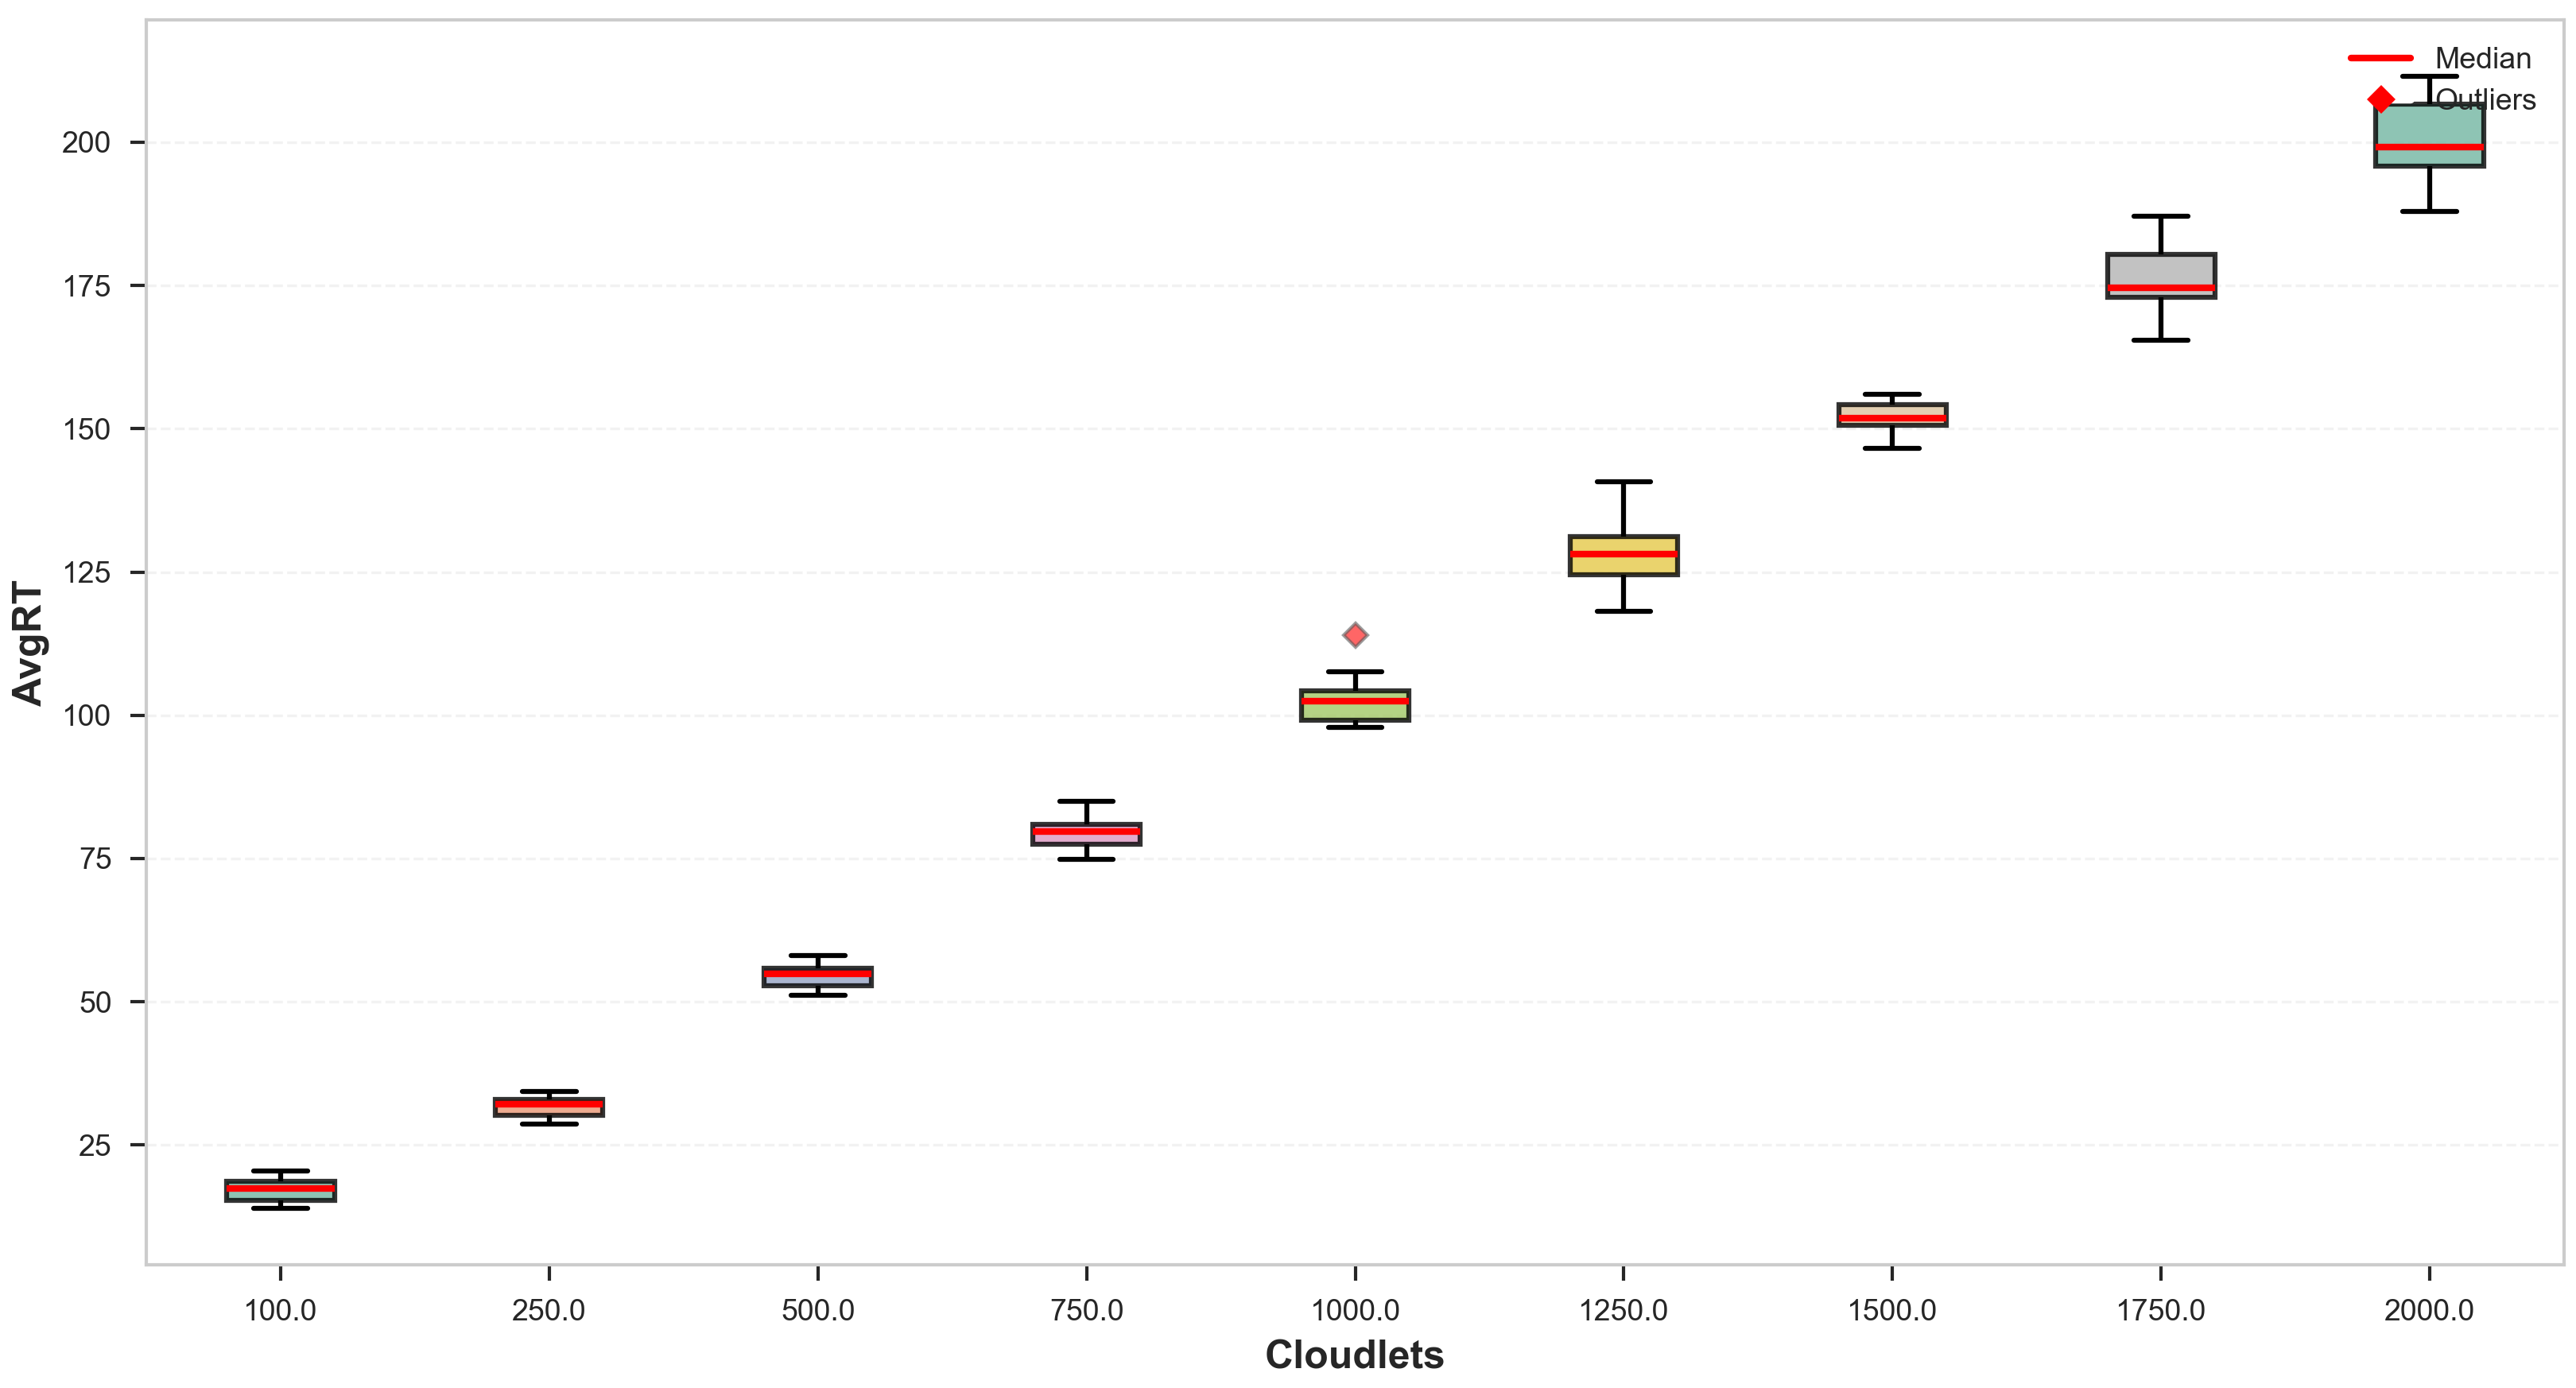
\includegraphics[
        width=\linewidth,
        trim=15 15 15 15,
        clip
    ]{Images/Results/boxplot_Cloudlets_AvgRT.png}
    \caption{Box-plot analysis of response time distribution}
    \label{fig:boxplot_rt}
\end{subfigure}
\caption{Response time analysis of RDA under varying cloudlet workloads}
\label{fig:response_analysis}
\end{figure}

Fig. \ref{fig:response_analysis} represents a scaling ratio of 0.588 suggesting favorable performance as the response time increases linearly rather than polynomially with increasing workload. This relationship indicates that scheduling efficiency is consistent at scale where large number of cloudlets are encountered. The response time scaling pattern is close to the makespan behavior observed in Section~\ref{subsec6.1}.

\subsubsection{Confidence Intervals and Reproducibility}

The RDA achieved 95\% confidence intervals across all workload configurations. The maximum confidence interval width was $\pm$0.54 ms, representing only 1.1\% of the mean response time. This indicates that RDA's scheduling decisions are highly deterministic and show minimal variance across independent simulation runs which is essential for reliable Service Level Agreement (SLA) compliance in production environments.

The box-plot analysis (Fig. ~\ref{fig:boxplot_rt}) shows symmetric distributions with minimal outliers throughout the tested range. The interquartile ranges remain tightly bounded relative to median values.

\subsubsection{Comparative Algorithm Performance}

The RDA showed a clear and consistent performance that is better than all the evaluated competitors. 

\begin{figure}[htbp]
\centering
\begin{subfigure}[t]{0.49\textwidth}
    \centering
    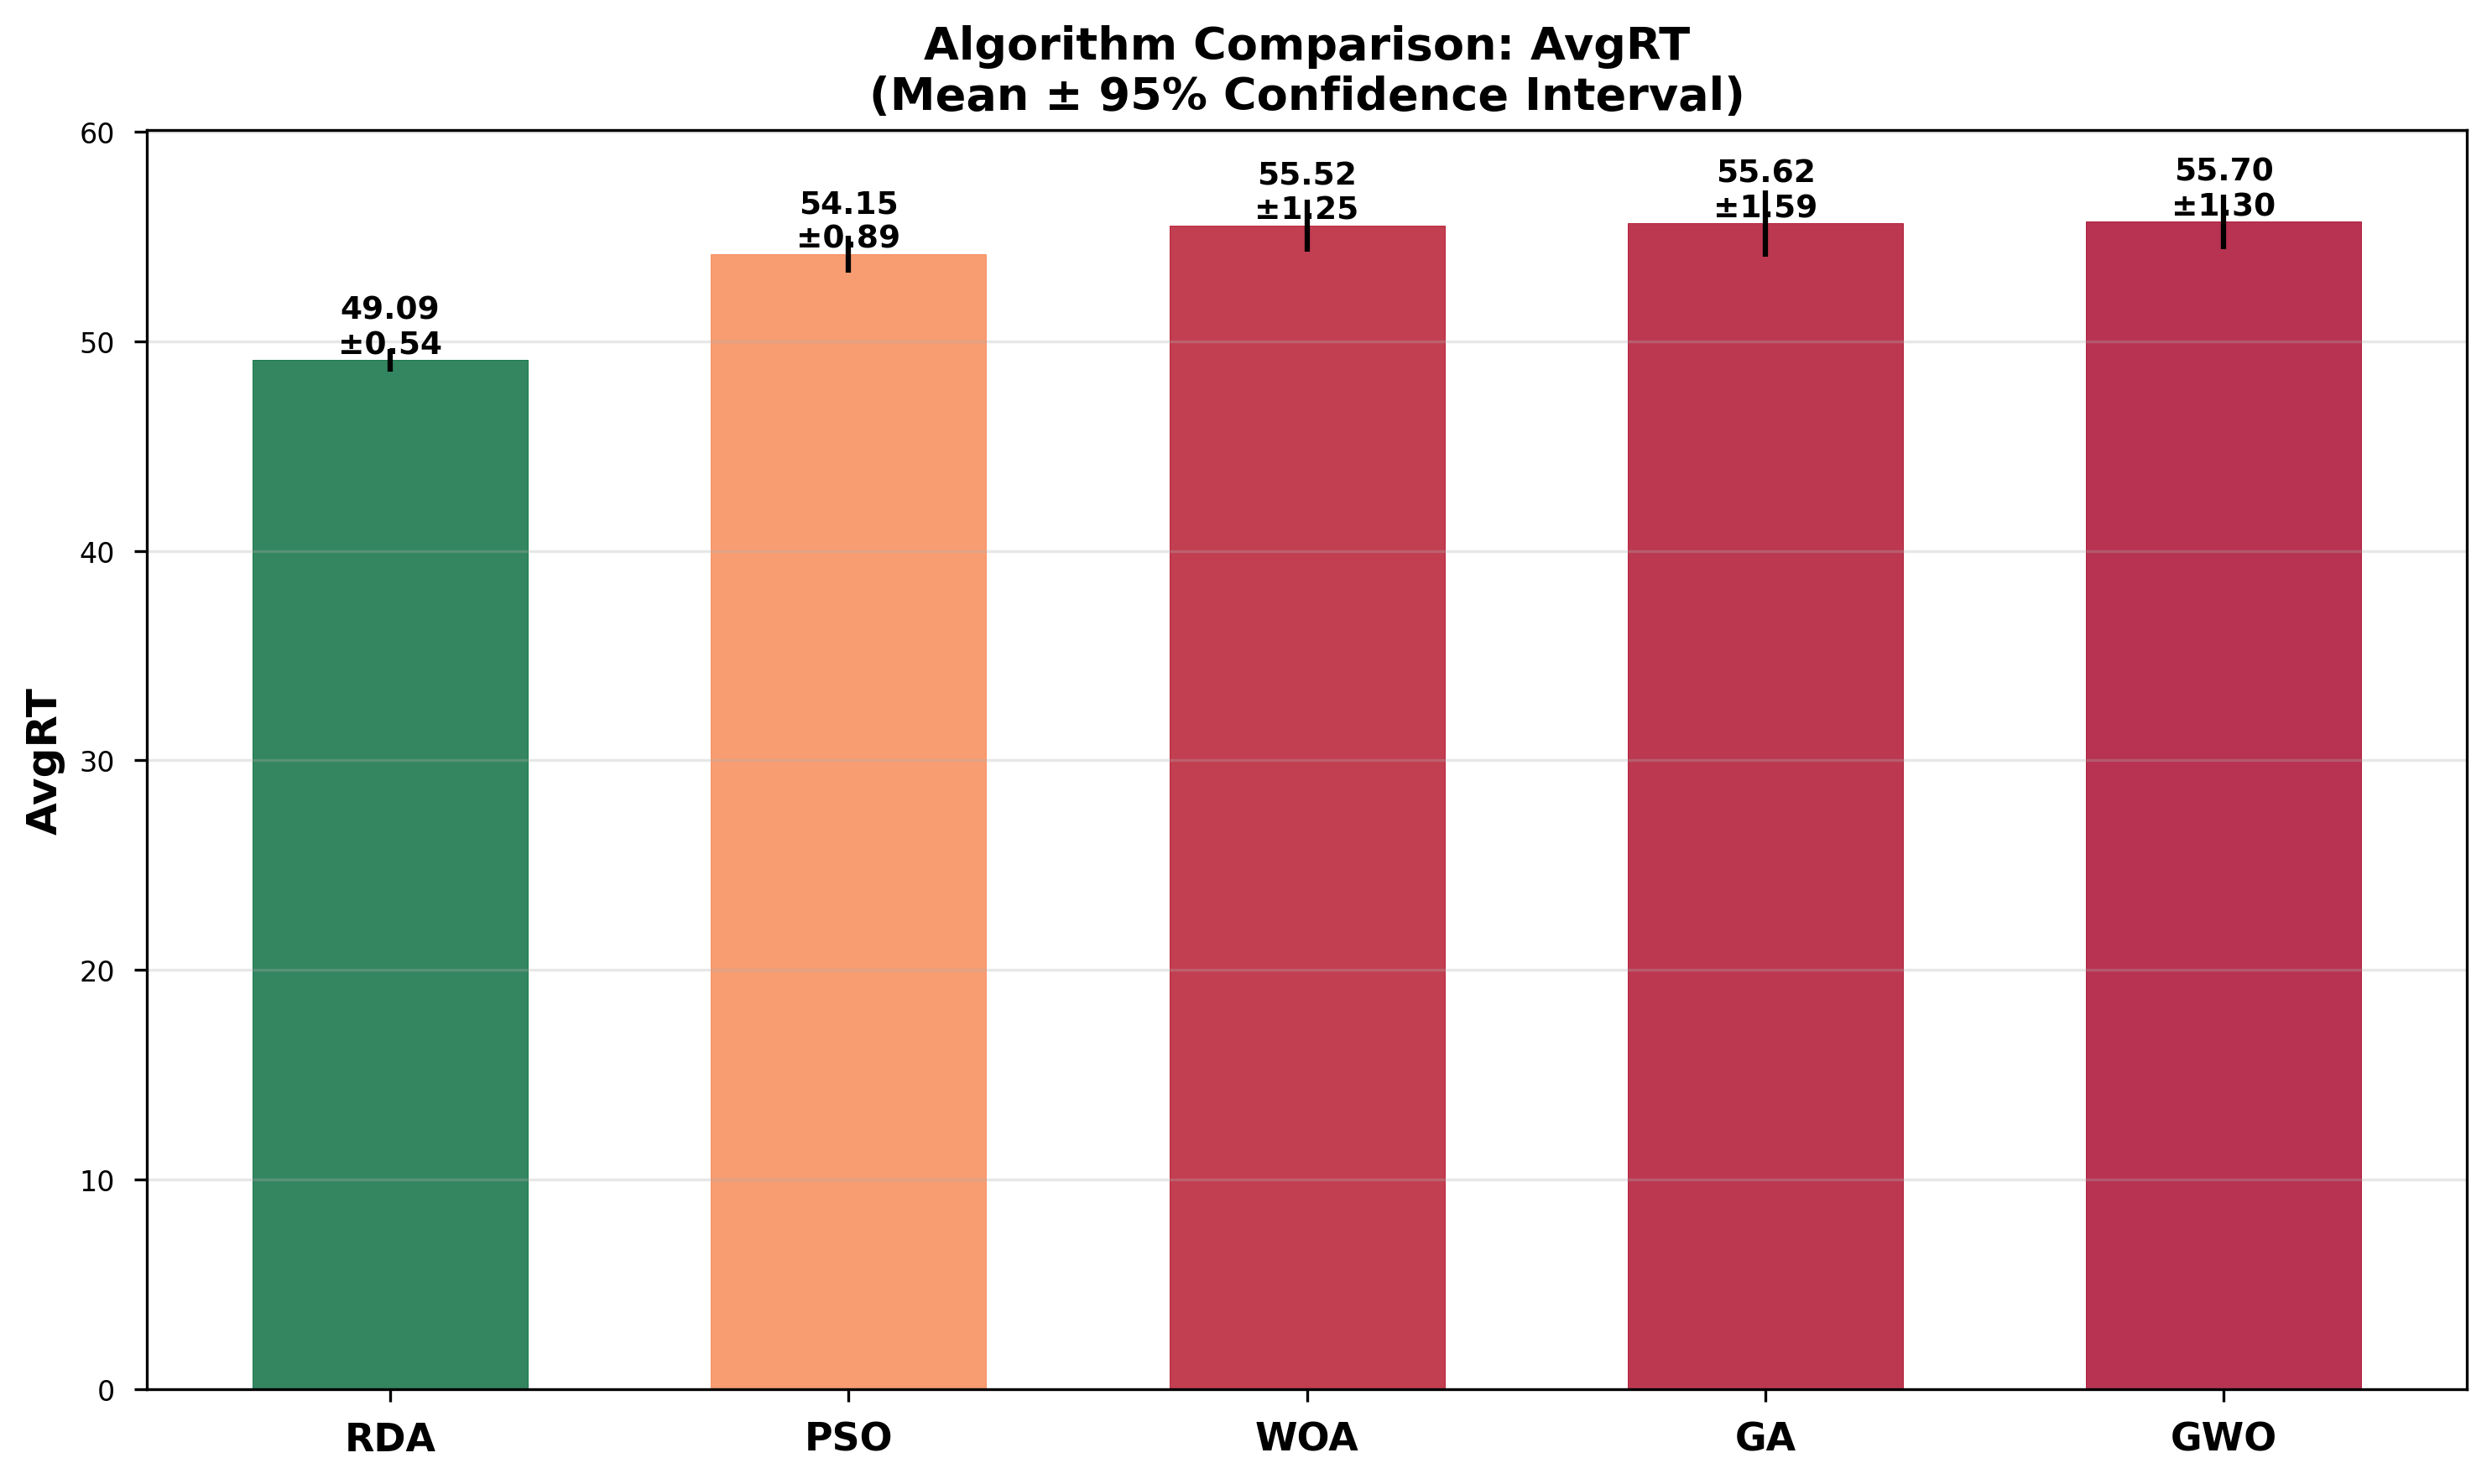
\includegraphics[
        width=\linewidth,
        trim=5 5 5 5,
        clip
    ]{Images/Results/Comparison/comparison_bars_AvgRT.png}
    \caption{Algorithm-wise response time comparison}
    \label{fig:comparison_rt}
\end{subfigure}
\hfill
\begin{subfigure}[t]{0.49\textwidth}
    \centering
    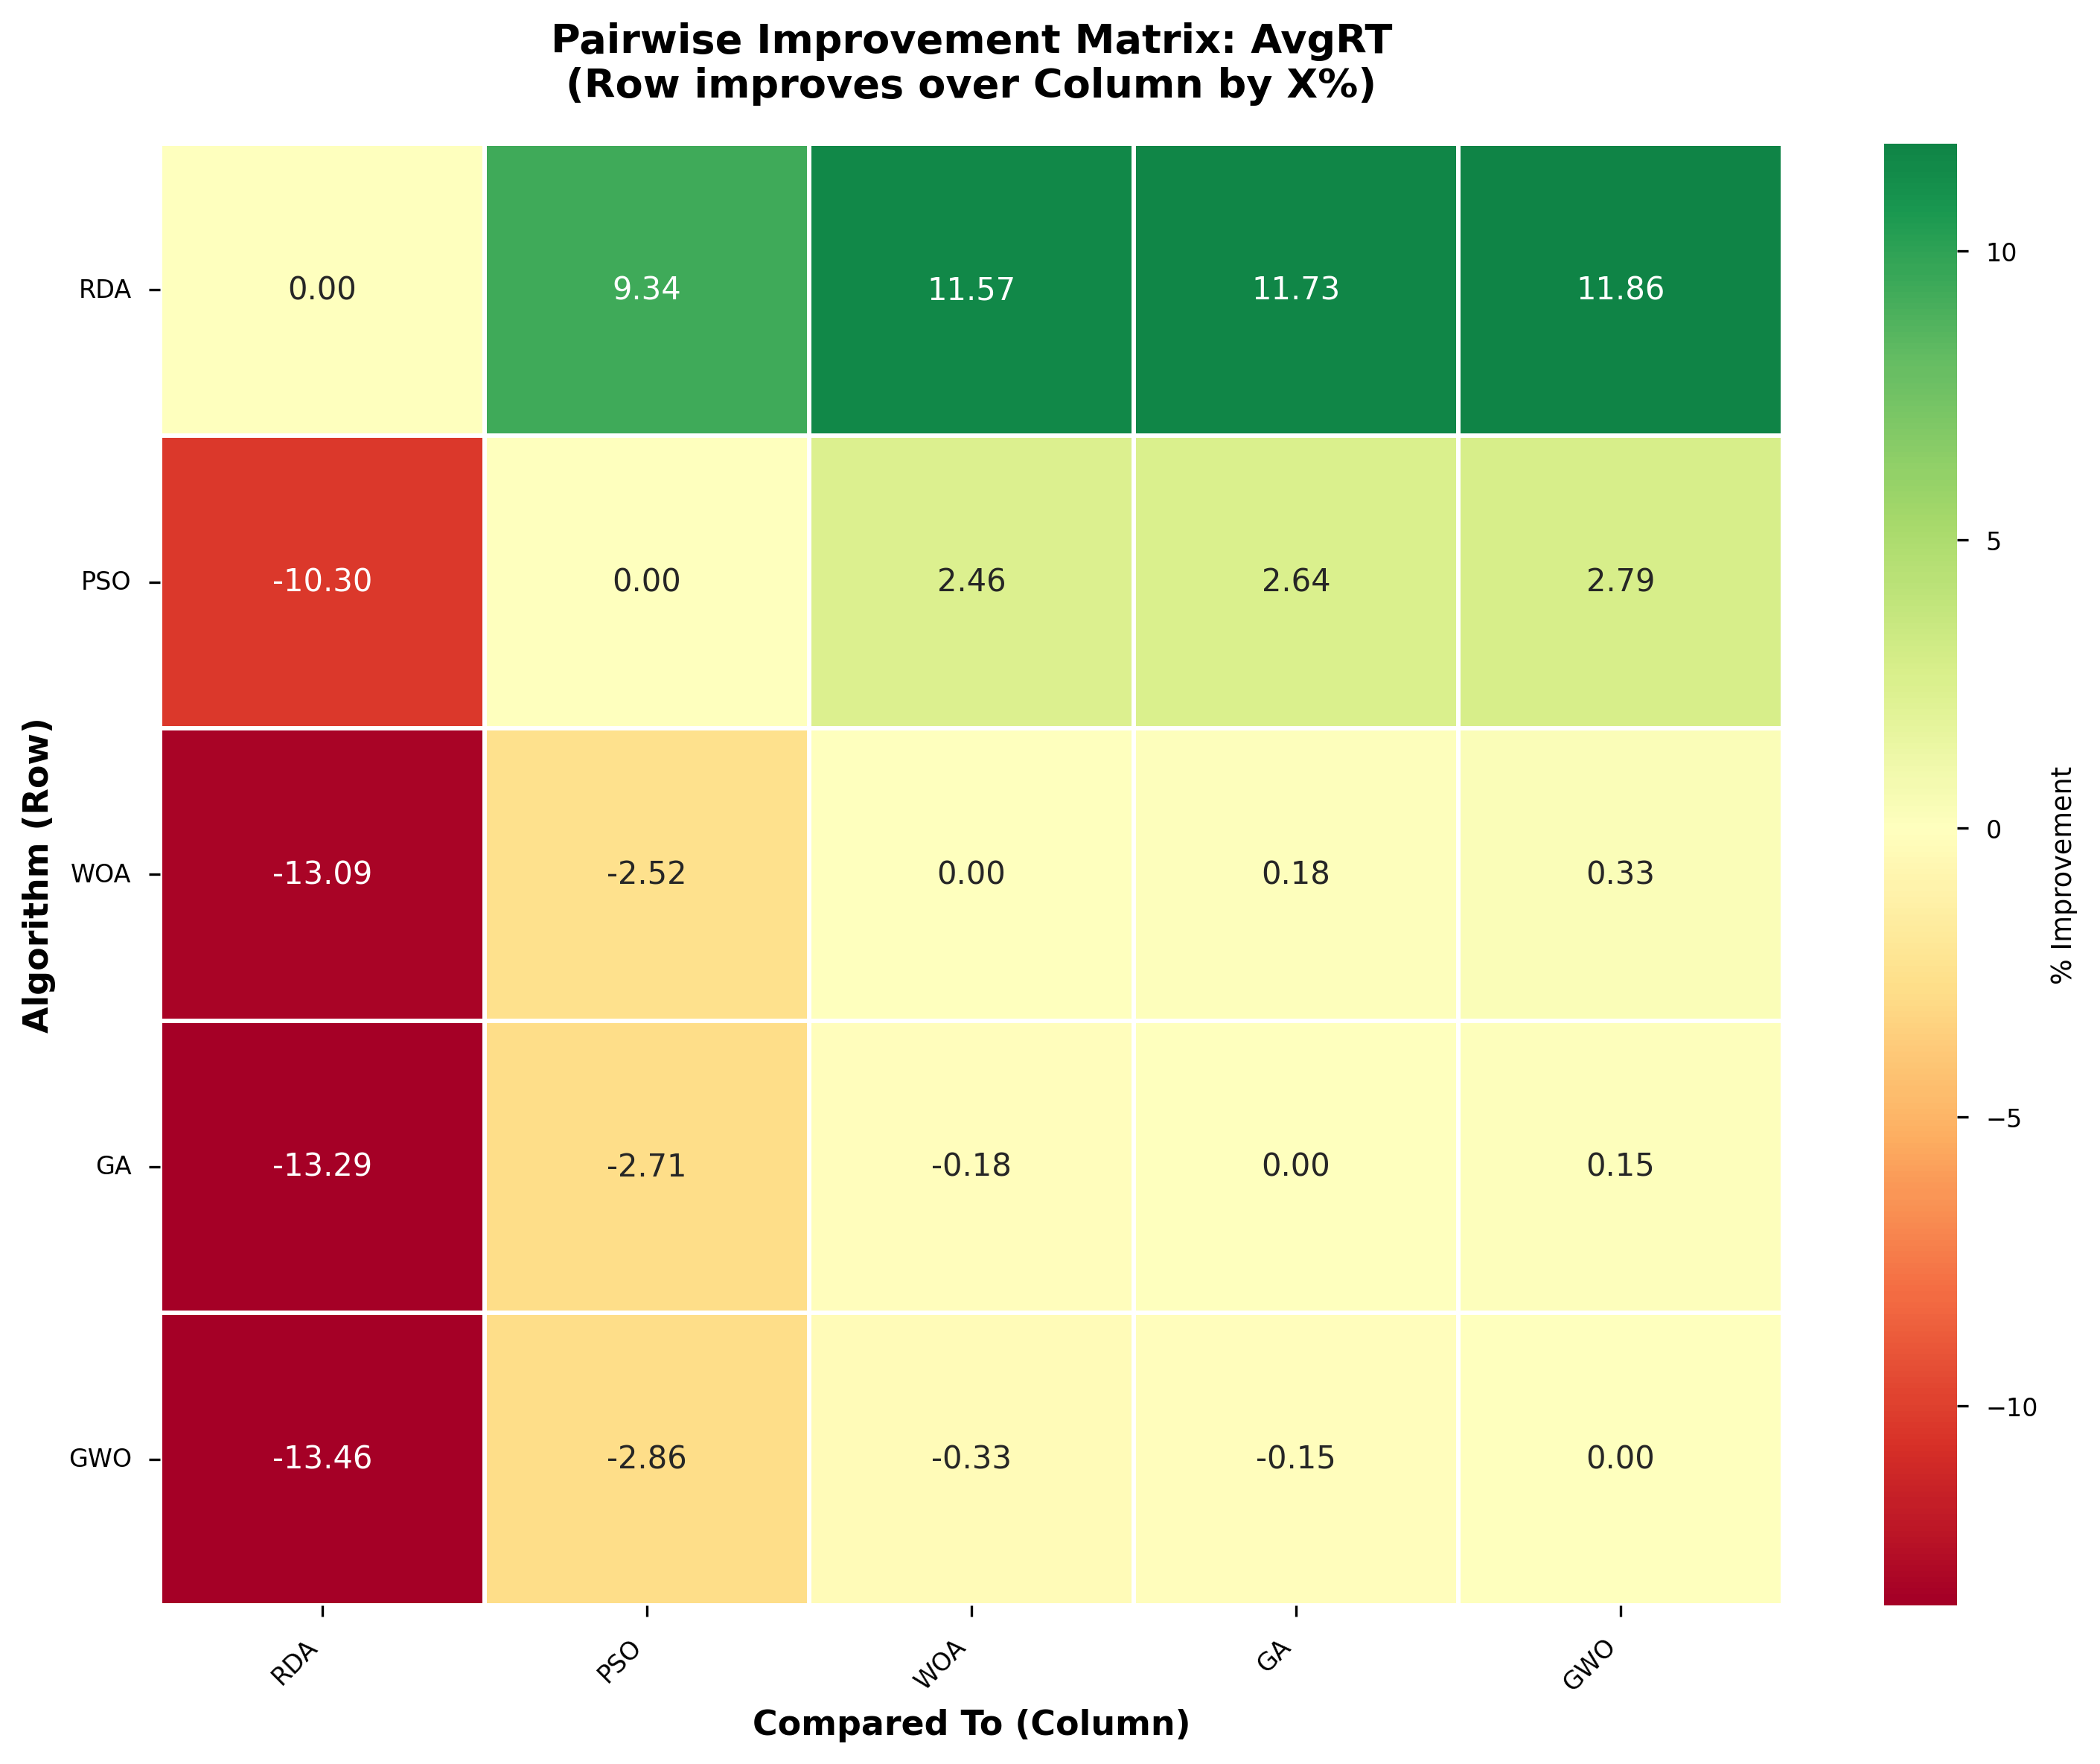
\includegraphics[
        width=\linewidth,
        trim=5 5 5 5,
        clip
    ]{Images/Results/Comparison/improvement_matrix_AvgRT.png}
    \caption{Percentage improvement matrix for response time}
    \label{fig:improvement_rt}
\end{subfigure}
\caption{Comparative response time analysis of the evaluated scheduling algorithms}
\label{fig:response_comparison}
\end{figure}

Table~\ref{tbl:response_time_comparison} presents mean response time values and comparative improvements.

\begin{table}[htbp]
\centering
\caption{Mean Response Time and Improvement Percentages Across Algorithms}
\label{tbl:response_time_comparison}
\begin{tabular}{l r r r}
\toprule
\textbf{Algorithm} & \textbf{Mean AvgRT (ms)} & \textbf{95\% CI} & \textbf{Improvement vs.~RDA (\%)} \\
\midrule
RDA & 49.09 & $\pm$0.54 & --- \\
PSO & 54.15 & $\pm$0.89 & $-9.34$ \\
WOA & 55.52 & $\pm$1.25 & $-11.57$ \\
GA & 55.62 & $\pm$1.59 & $-11.73$ \\
GWO & 55.70 & $\pm$1.30 & $-11.86$ \\
\bottomrule
\end{tabular}
\end{table}

As mentioned in Table \ref{tbl:response_time_comparison} RDA achieved a mean average response time of 49.09 ms ($\pm$0.54 ms), representing substantial improvements over all competitors: 9.34\% over PSO, 11.57\% over WOA, 11.73\% over GA, and 11.86\% over GWO. The improvement percentages shows consistent better performance of RDA in comparison to all other algorithms.

The coefficient of variation (ratio of standard deviation to mean, estimated from confidence interval data) is approximately 1.1\% for RDA, compared to 1.64\%-2.86\% for competing algorithms. RDA's confidence intervals are 33\% tighter than PSO (best competitor) and three times tighter than GA (least stable competitor), indicating that scheduling decisions are made with comparatively low variance.

In production environments where both average performance and predictability are mandated through SLAs, RDA provides not only faster response times but also greater confidence in meeting performance guaranties.

Fig. ~\ref{fig:response_comparison} presents a detailed comparative analysis, with the improvement matrix Figure~\ref{fig:improvement_rt} representing percentage gains across all algorithm pairs and workloads.

\subsection{Convergence Analysis}\label{subsec6.3}

Convergence analysis evaluates the RDA's capability to iteratively improve scheduling solutions with each successive iteration. The analysis examines convergence behavior and population size sensitivity.

\begin{figure}[htbp]
\centering
\begin{subfigure}[t]{0.49\textwidth}
    \centering
    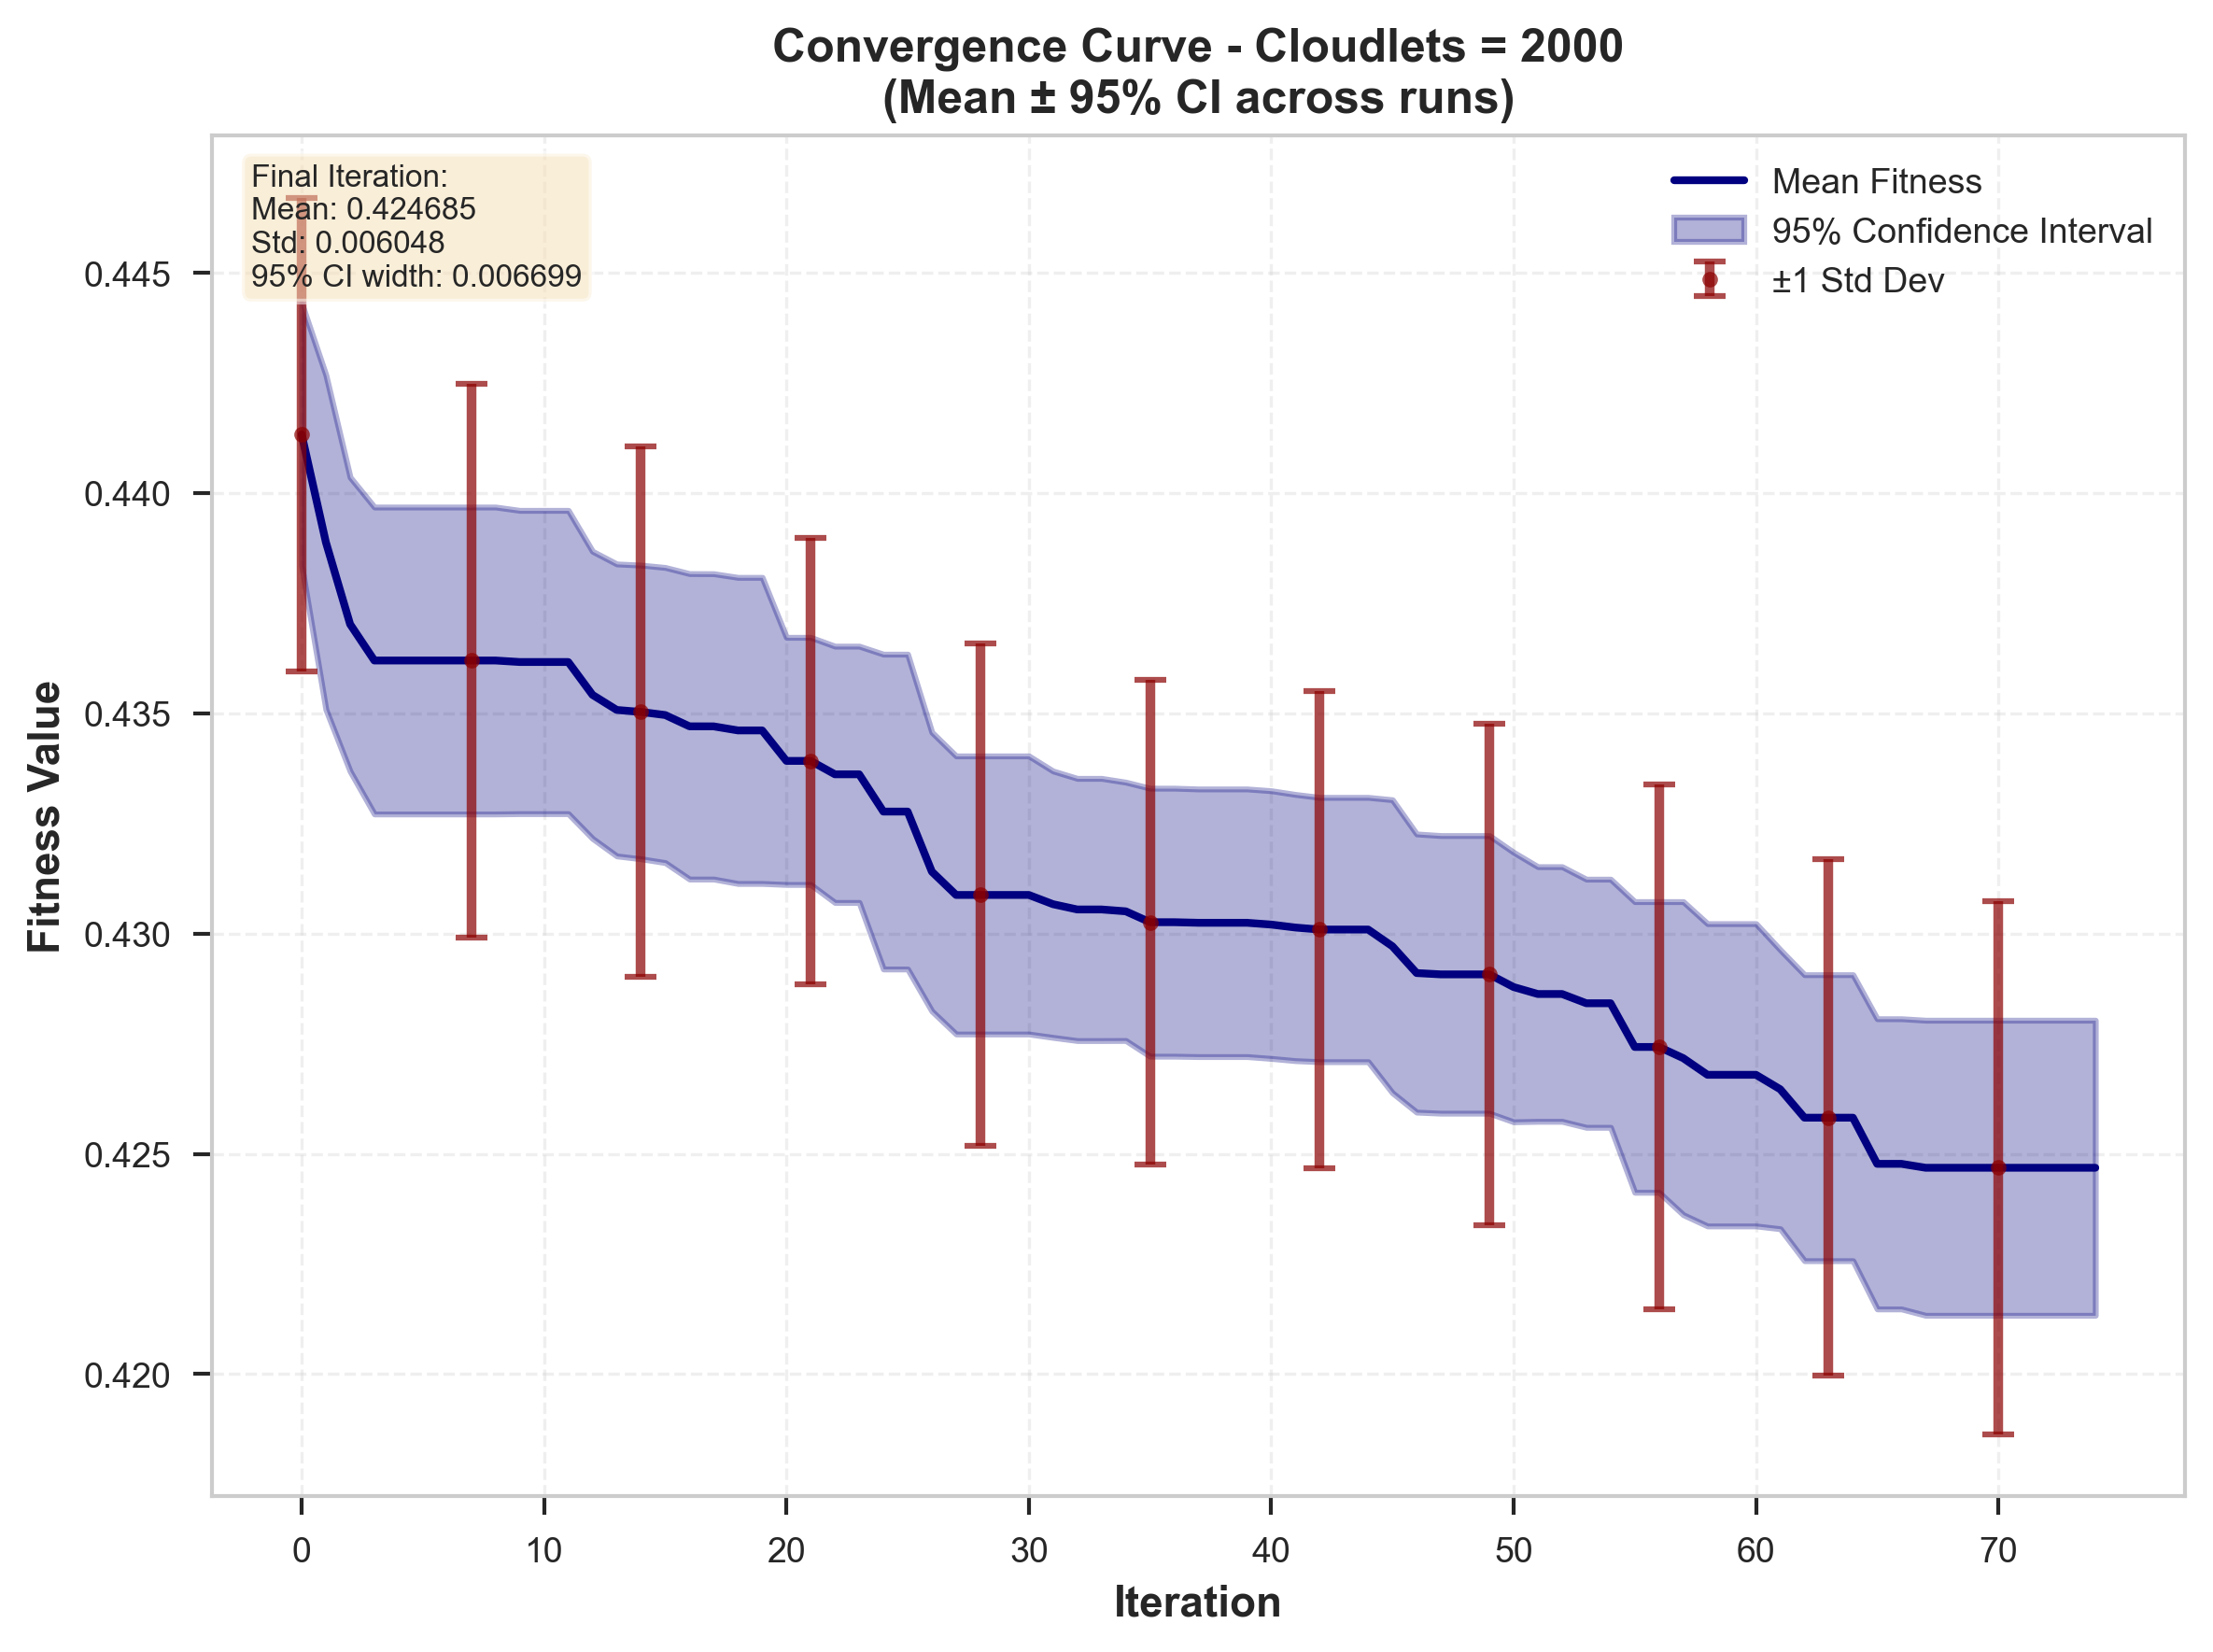
\includegraphics[width=\linewidth, trim=15 15 15 15, clip]{Images/Results/Convergence/convergence_Cloudlets_2000.png}
    \caption{Convergence behavior (2000 cloudlets)}
    \label{fig:conv_cloudlets}
\end{subfigure}
\hfill
\begin{subfigure}[t]{0.49\textwidth}
    \centering
    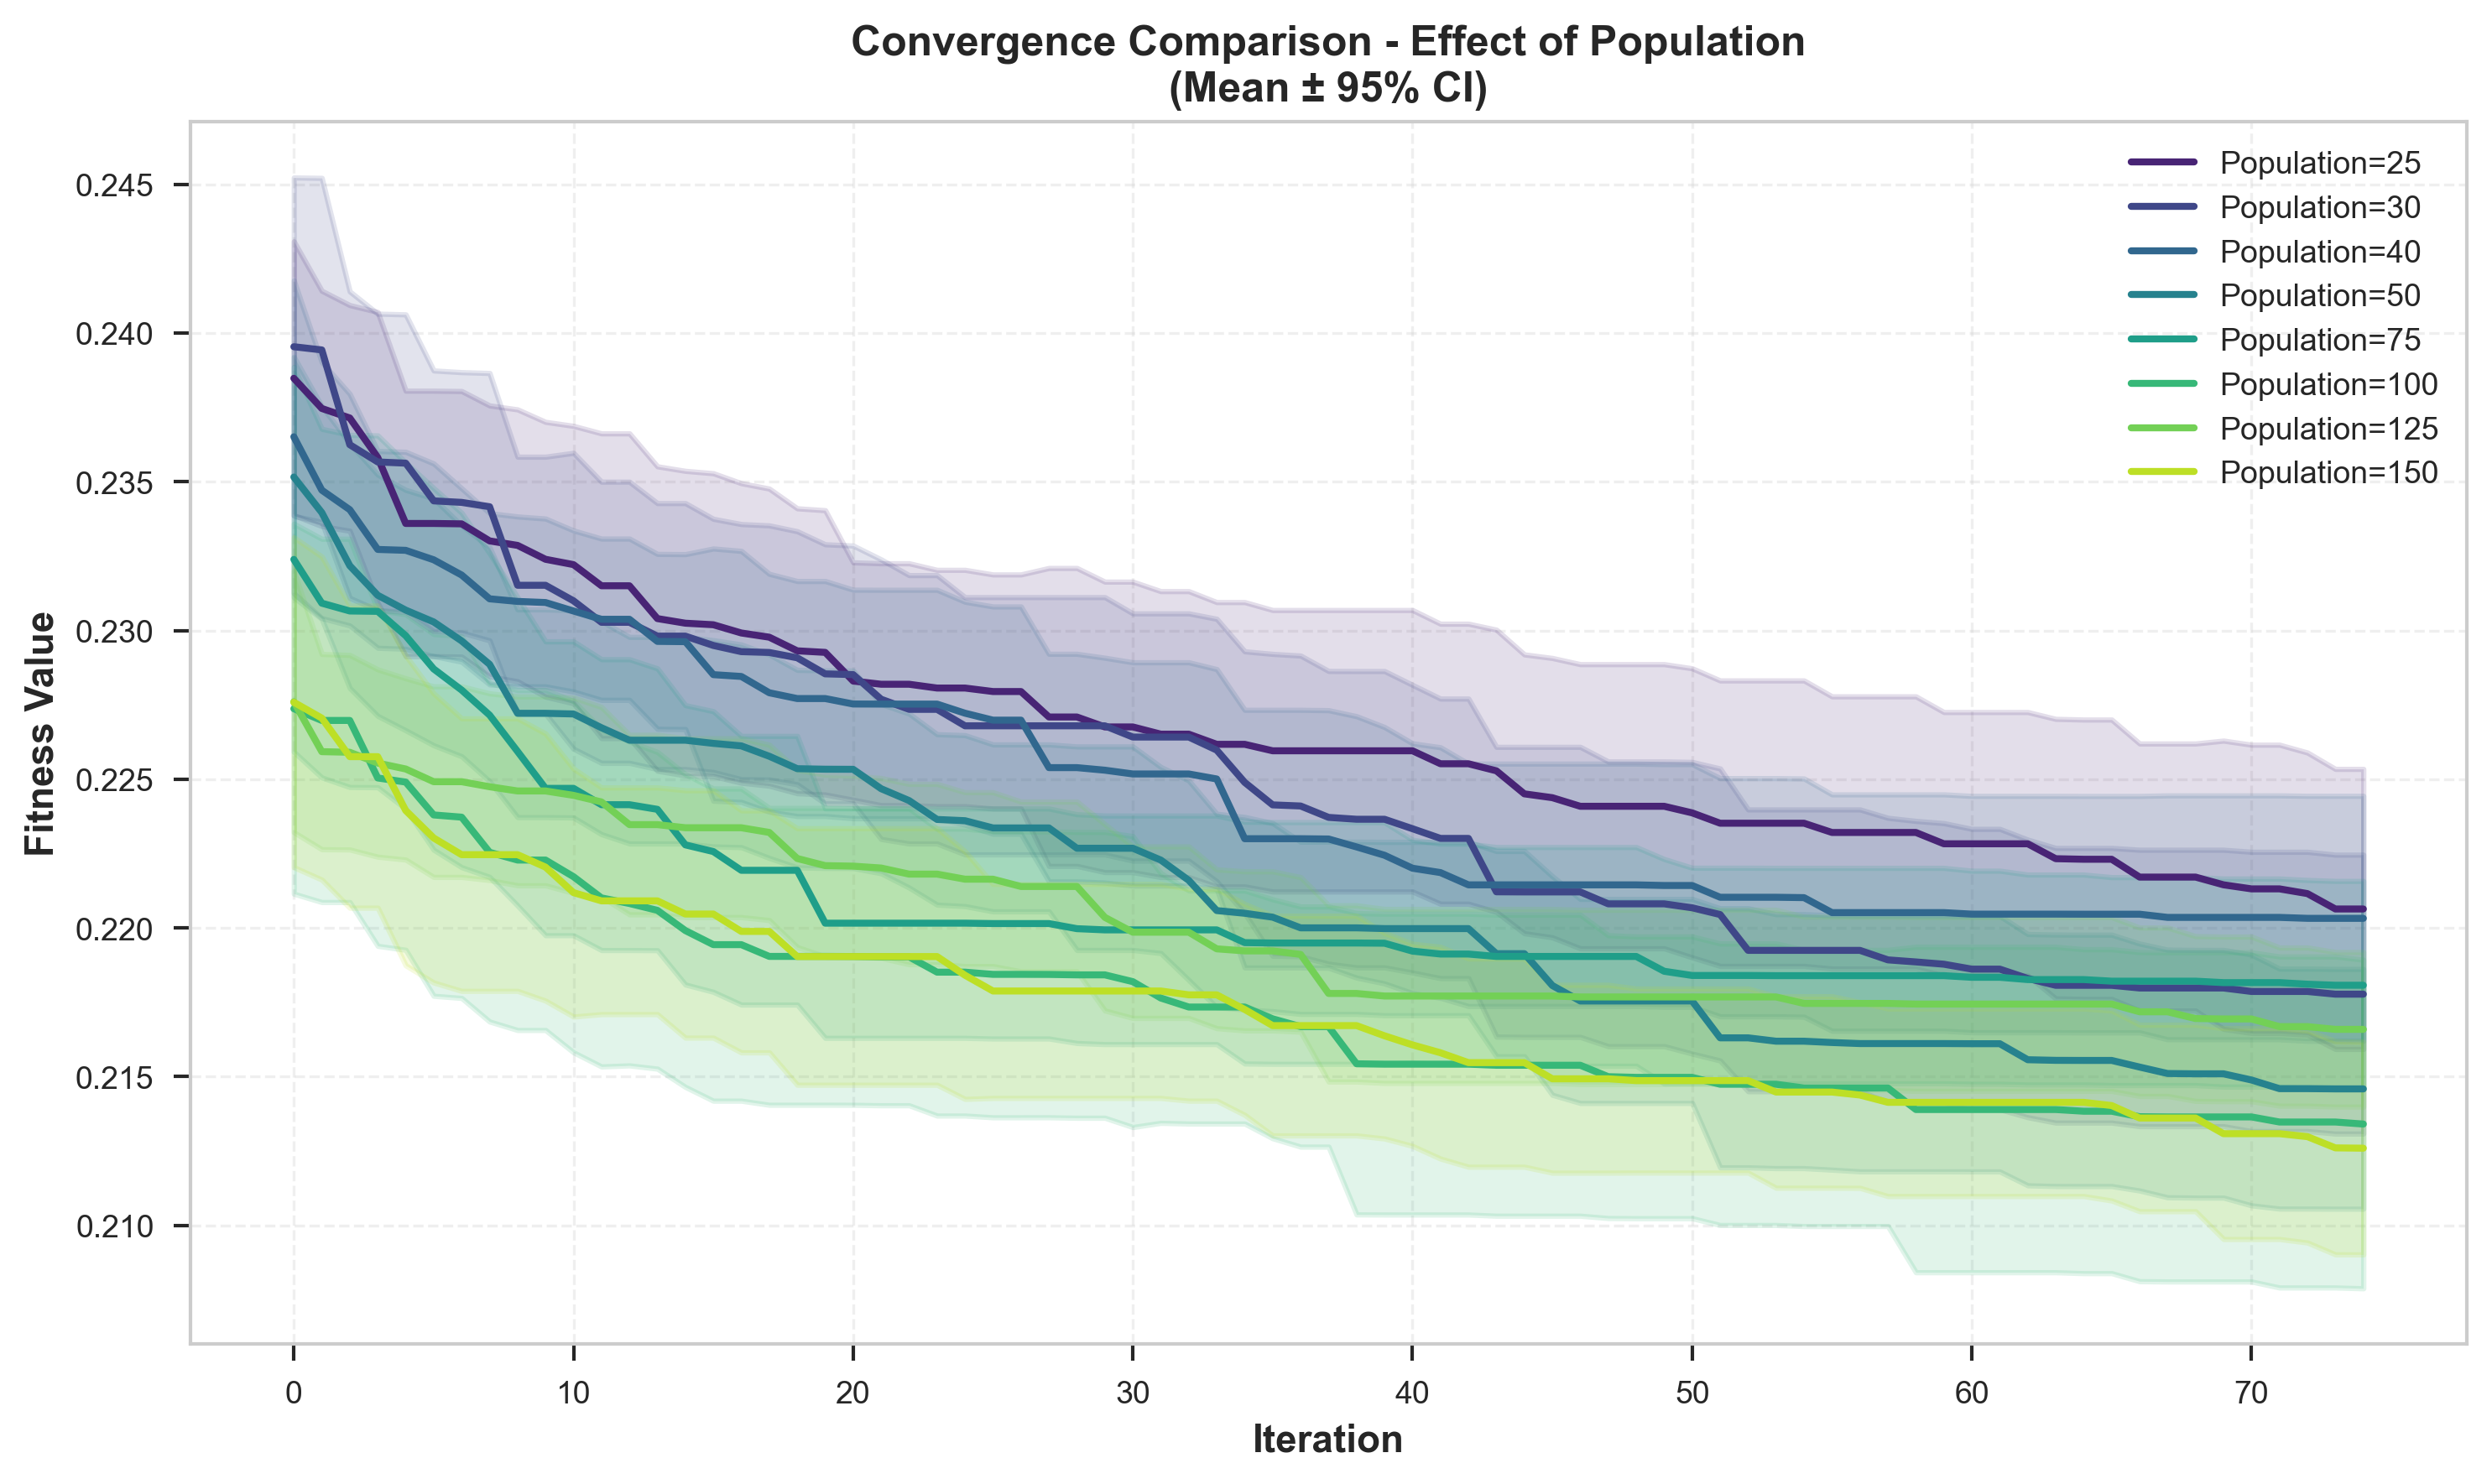
\includegraphics[width=\linewidth, trim=15 15 15 15, clip]{Images/Results/Convergence/convergence_comparison_Population.png}
    \caption{Population size sensitivity}
    \label{fig:conv_population}
\end{subfigure}
\caption{Convergence analysis under different configurations}
\label{fig:convergence_analysis}
\end{figure}

\textbf{Primary Convergence Behavior:} Figure~\ref{fig:convergence_analysis} presents convergence characteristics for the 2,000 cloudlet workload using population size 100 (Table~\ref{tab:algo_params}). The RDA exhibited rapid fitness improvement during iterations 0-30, with fitness decreasing from 0.4412 to 0.4309 (2.3\% improvement). Convergence plateaued first after iteration 40 and finally after iteration 70, subsequent iterations produced marginal refinements that accumulated to final fitness value of 0.4247 (3.7\% cumulative improvement, $\pm$0.0007). This pattern of rapid exploration followed by exploitation, reflects effective metaheuristic behavior where the algorithm identifies promising solution regions early and refines solutions within those regions.

\textbf{Population Size Sensitivity:} Fig. ~\ref{fig:conv_population} presents convergence across eight population sizes ranged from 25 to 150 individuals with 2,000 cloudlet per simulation. Smaller populations (25-40) converge rapidly to suboptimal solutions, while larger populations (100-150) achieve substantially better final solutions. Populations 100-150 achieved optimal fitness values within 0.6\% vicinity of each other, indicating diminishing returns beyond population=100. Hence, the final size for population is chosen as 100 which performs best and provdies an optimal scheduling solution while maintaining computational efficiency.

\subsection{Parameter Sensitivity Analysis}\label{subsec6.4}

Values for the parameters used in RDA model are experimentally evaluated by trying different combinations of values for each parameter. Below is the analysis for values of parameters alpha, beta and gamma and their sensitivity. All the parameters with their chosen value are listed in Table \ref{tab:algo_params}. 

The major factor for determining the sensitivity is here considered as makespan because of it's weight as QoS factor. All the factor i.e. makespan, response time, cost and utilization were considered while determining the value for parameters experimentally.

\begin{figure}[htbp]
\centering
\begin{subfigure}[b]{0.47\textwidth}
    \centering
    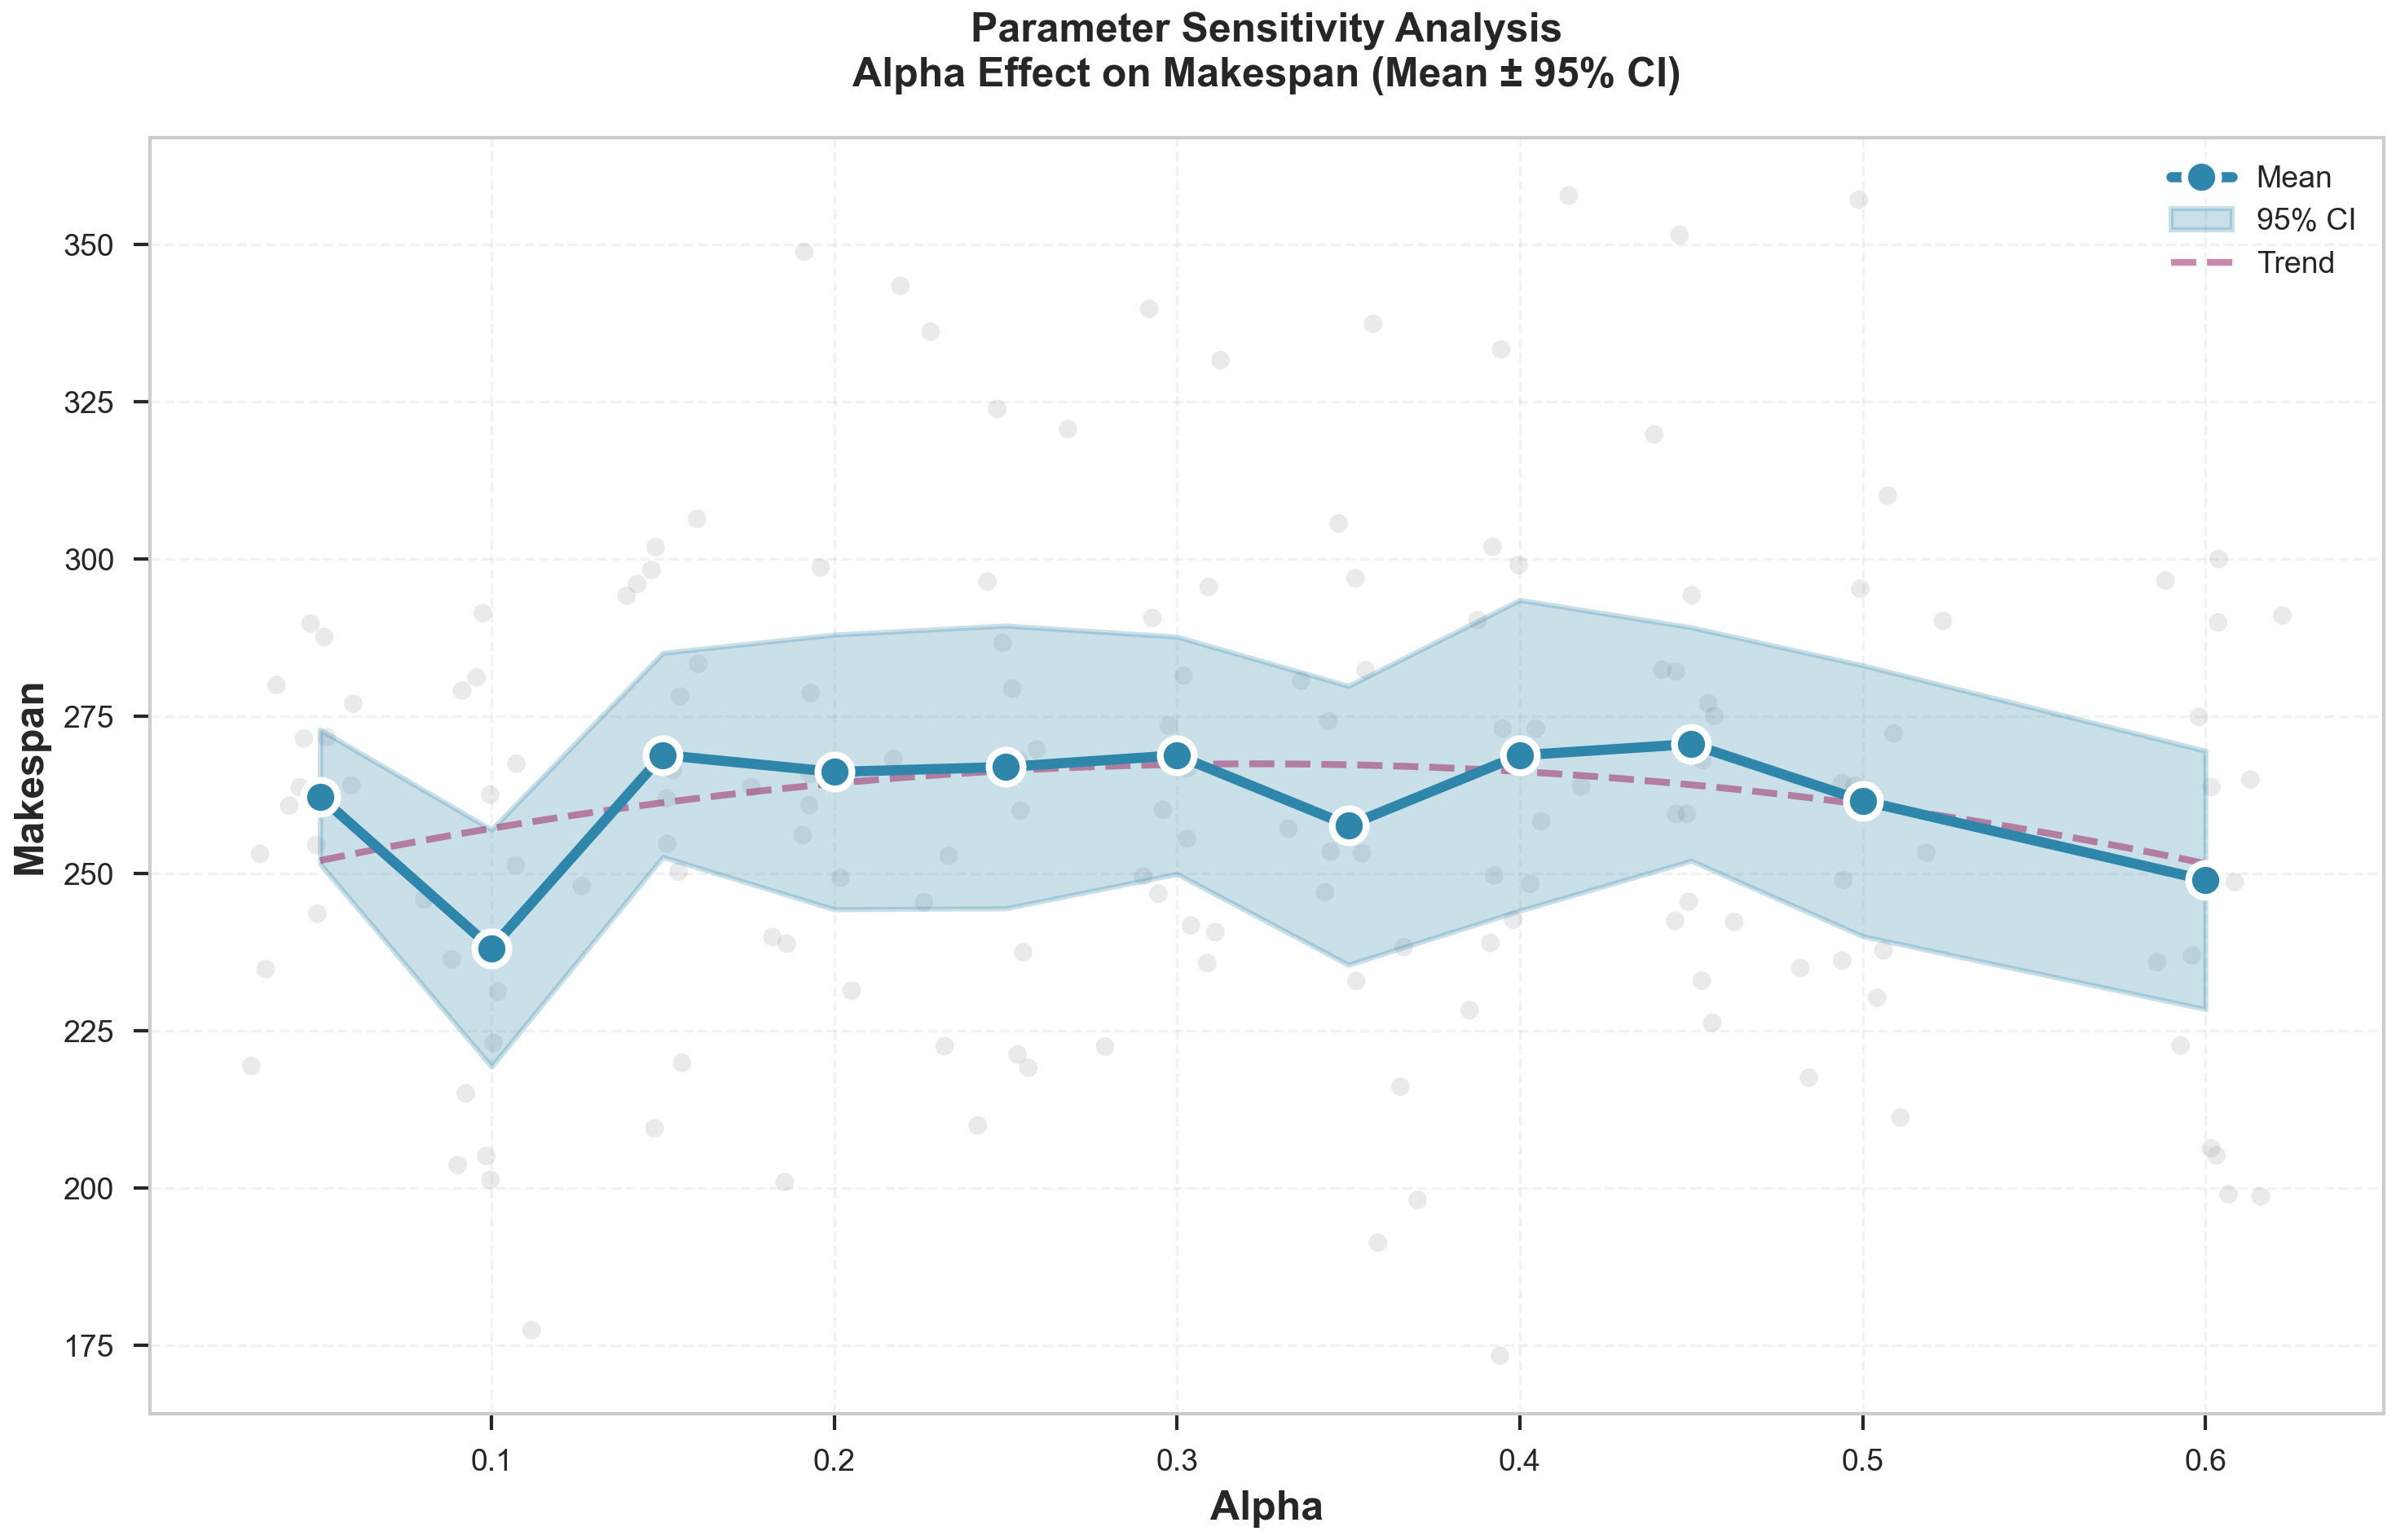
\includegraphics[width=0.95\textwidth]{Images/Results/ParameterAnalysis/Alpha_Makespan.png}
    \caption{Alpha sensitivity}
    \label{fig:alpha_ms}
\end{subfigure}
\hfill
\begin{subfigure}[b]{0.47\textwidth}
    \centering
    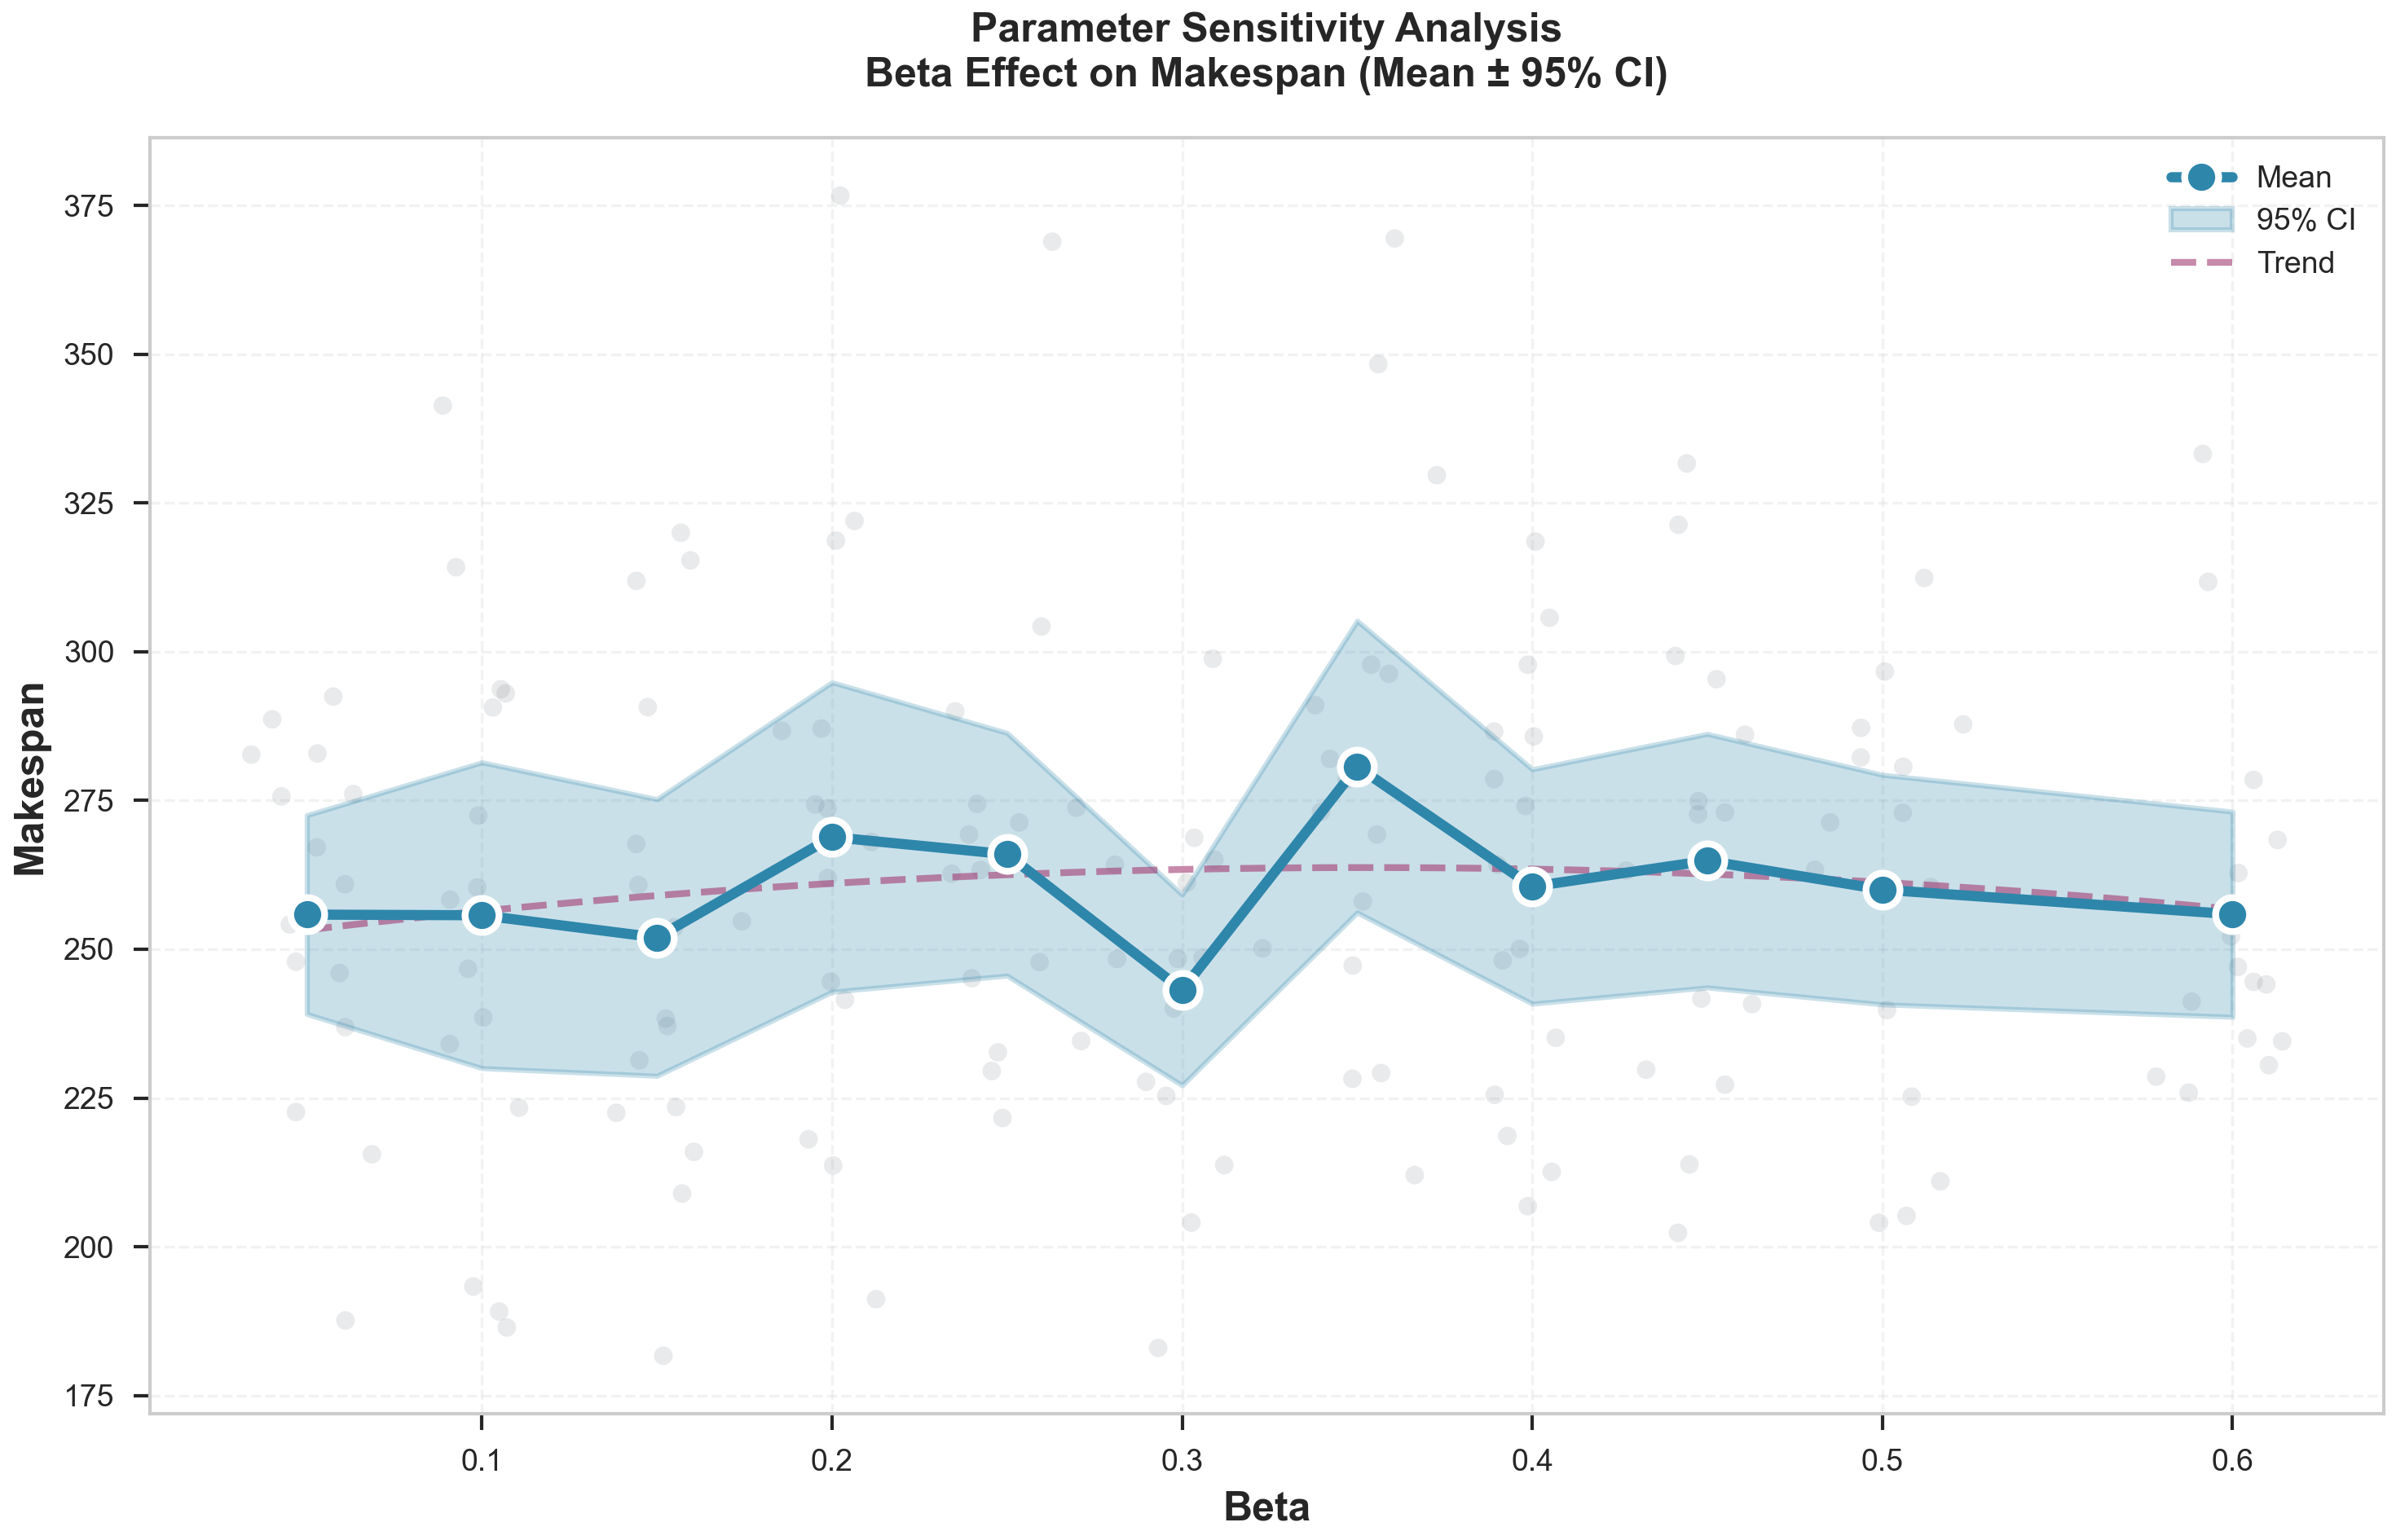
\includegraphics[width=0.95\textwidth]{Images/Results/ParameterAnalysis/Beta_Makespan.png}
    \caption{Beta sensitivity}
    \label{fig:beta_ms}
\end{subfigure}
\vspace{0.2cm}
\begin{subfigure}[b]{0.47\textwidth}
    \centering
    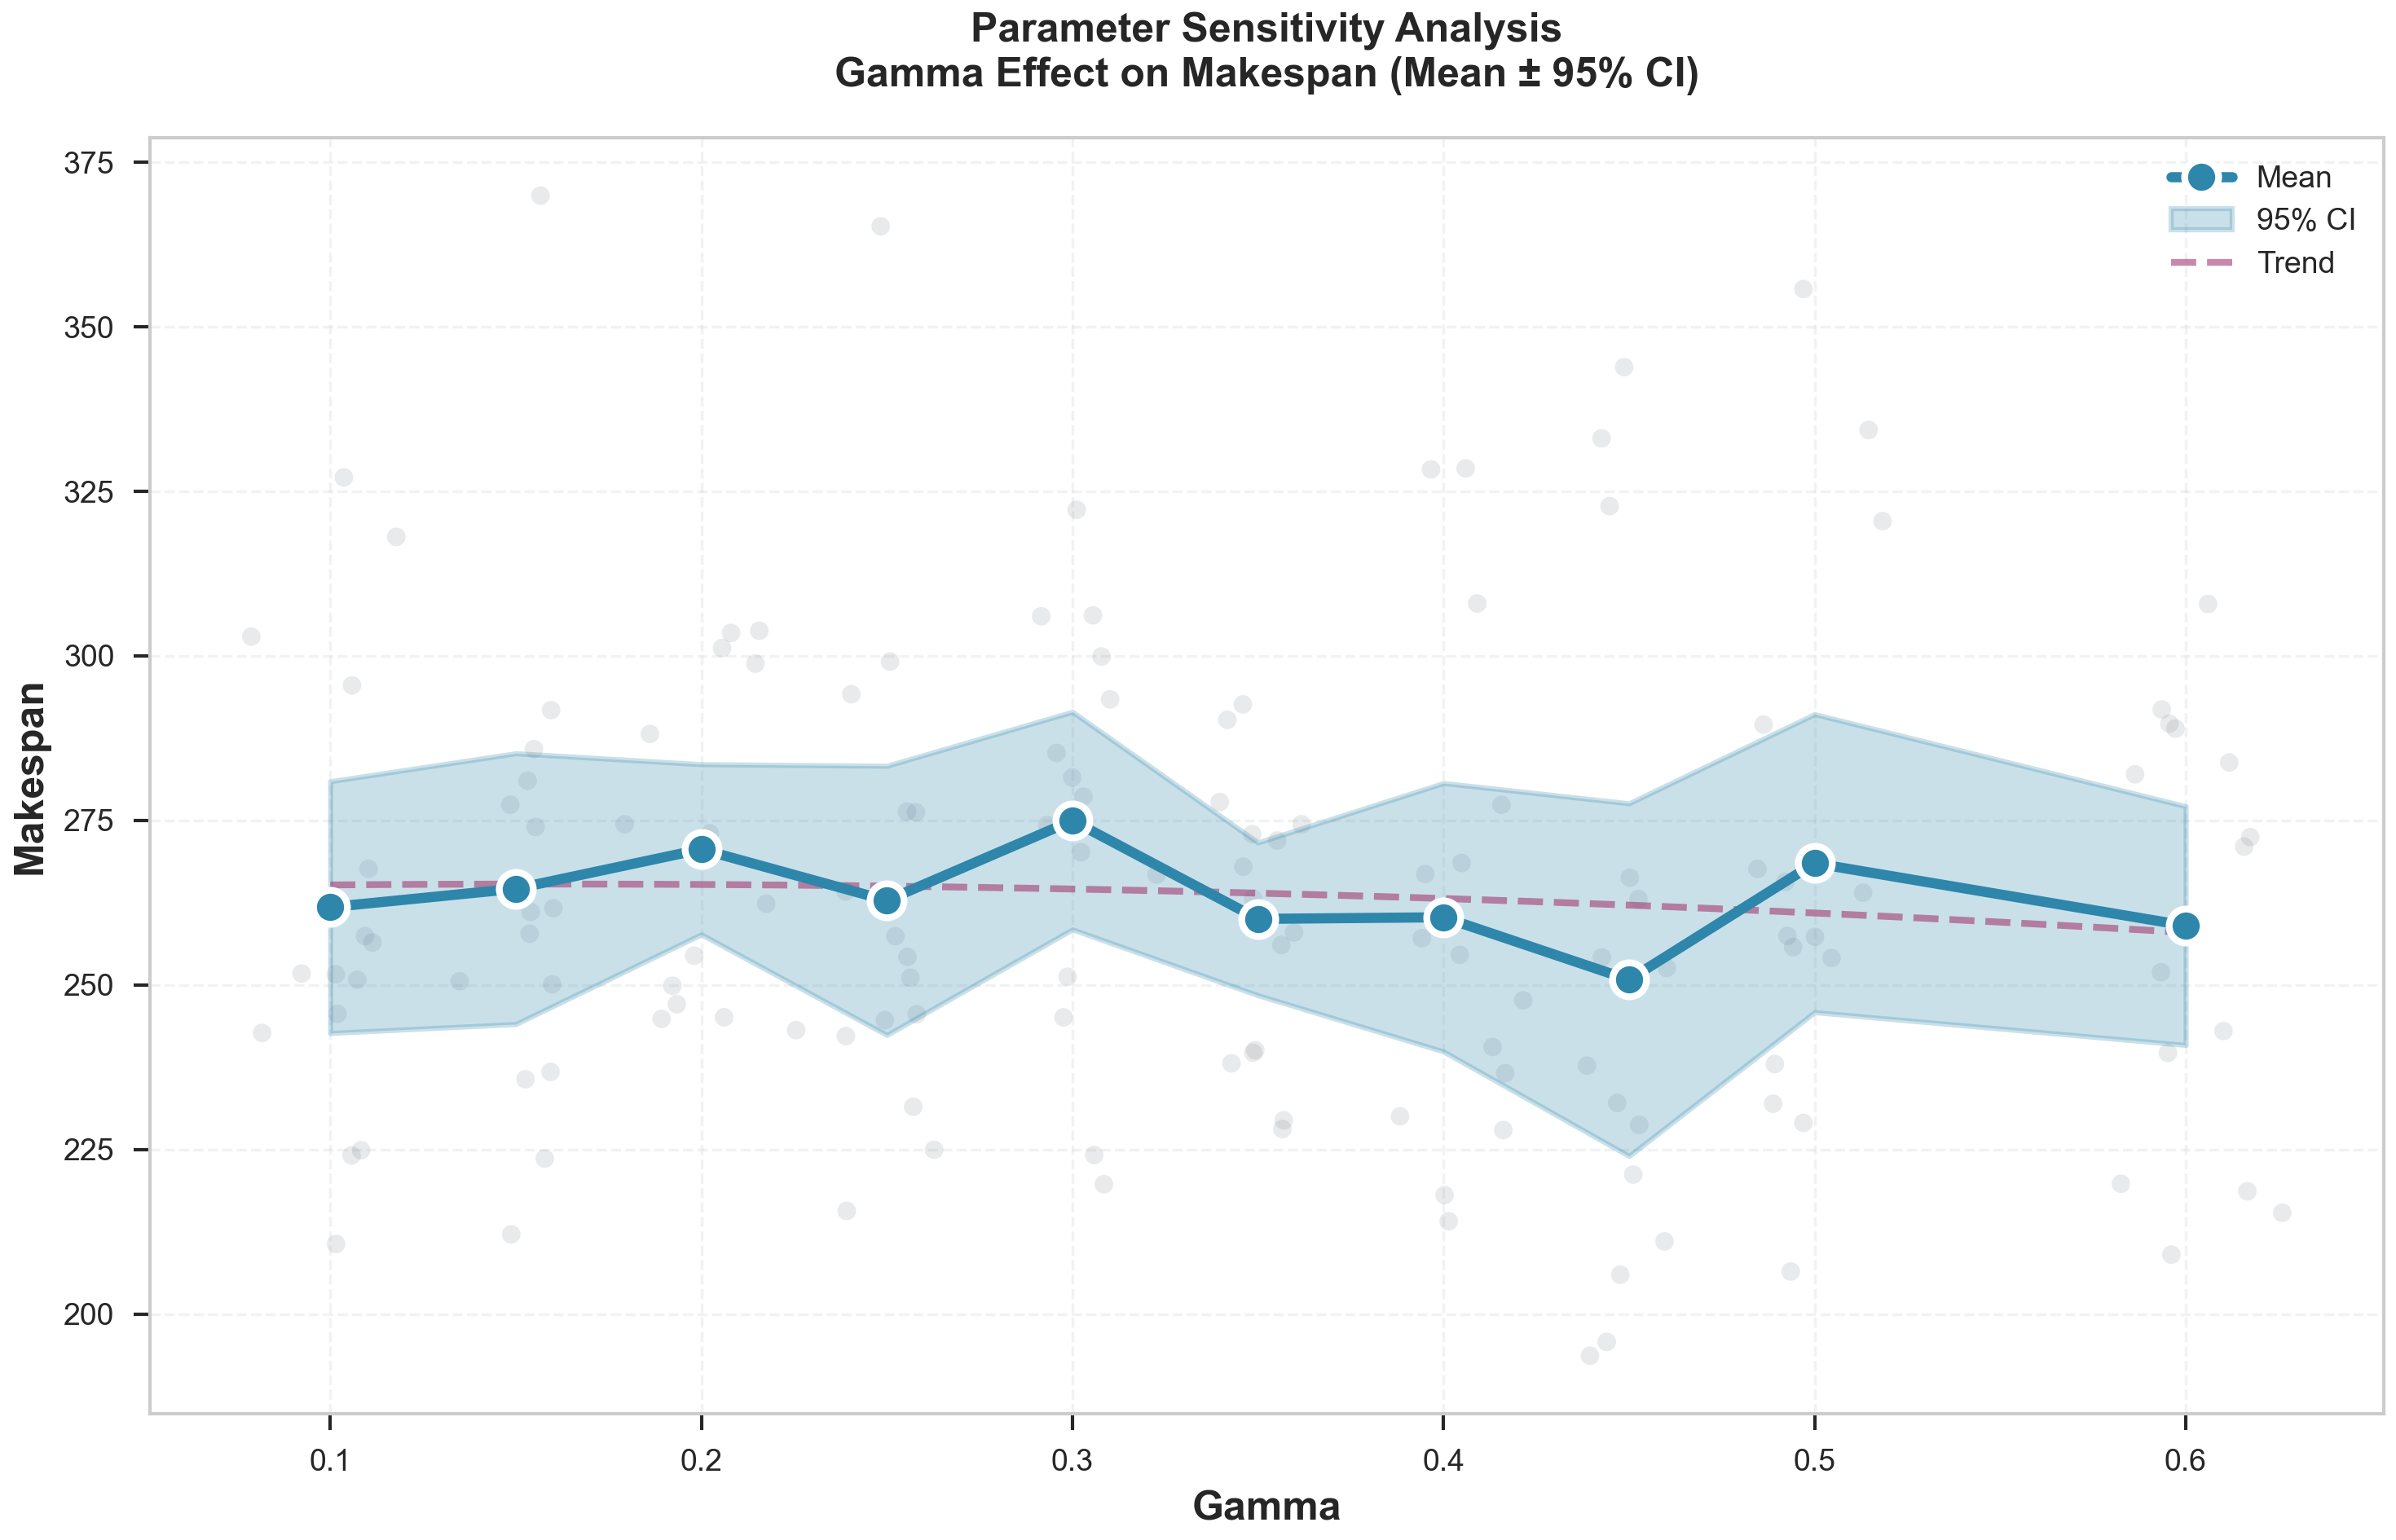
\includegraphics[width=0.95\textwidth]{Images/Results/ParameterAnalysis/Gamma_Makespan.png}
    \caption{Gamma sensitivity}
    \label{fig:gamma_ms}
\end{subfigure}
\hfill
\begin{subfigure}[b]{0.47\textwidth}
    \centering
    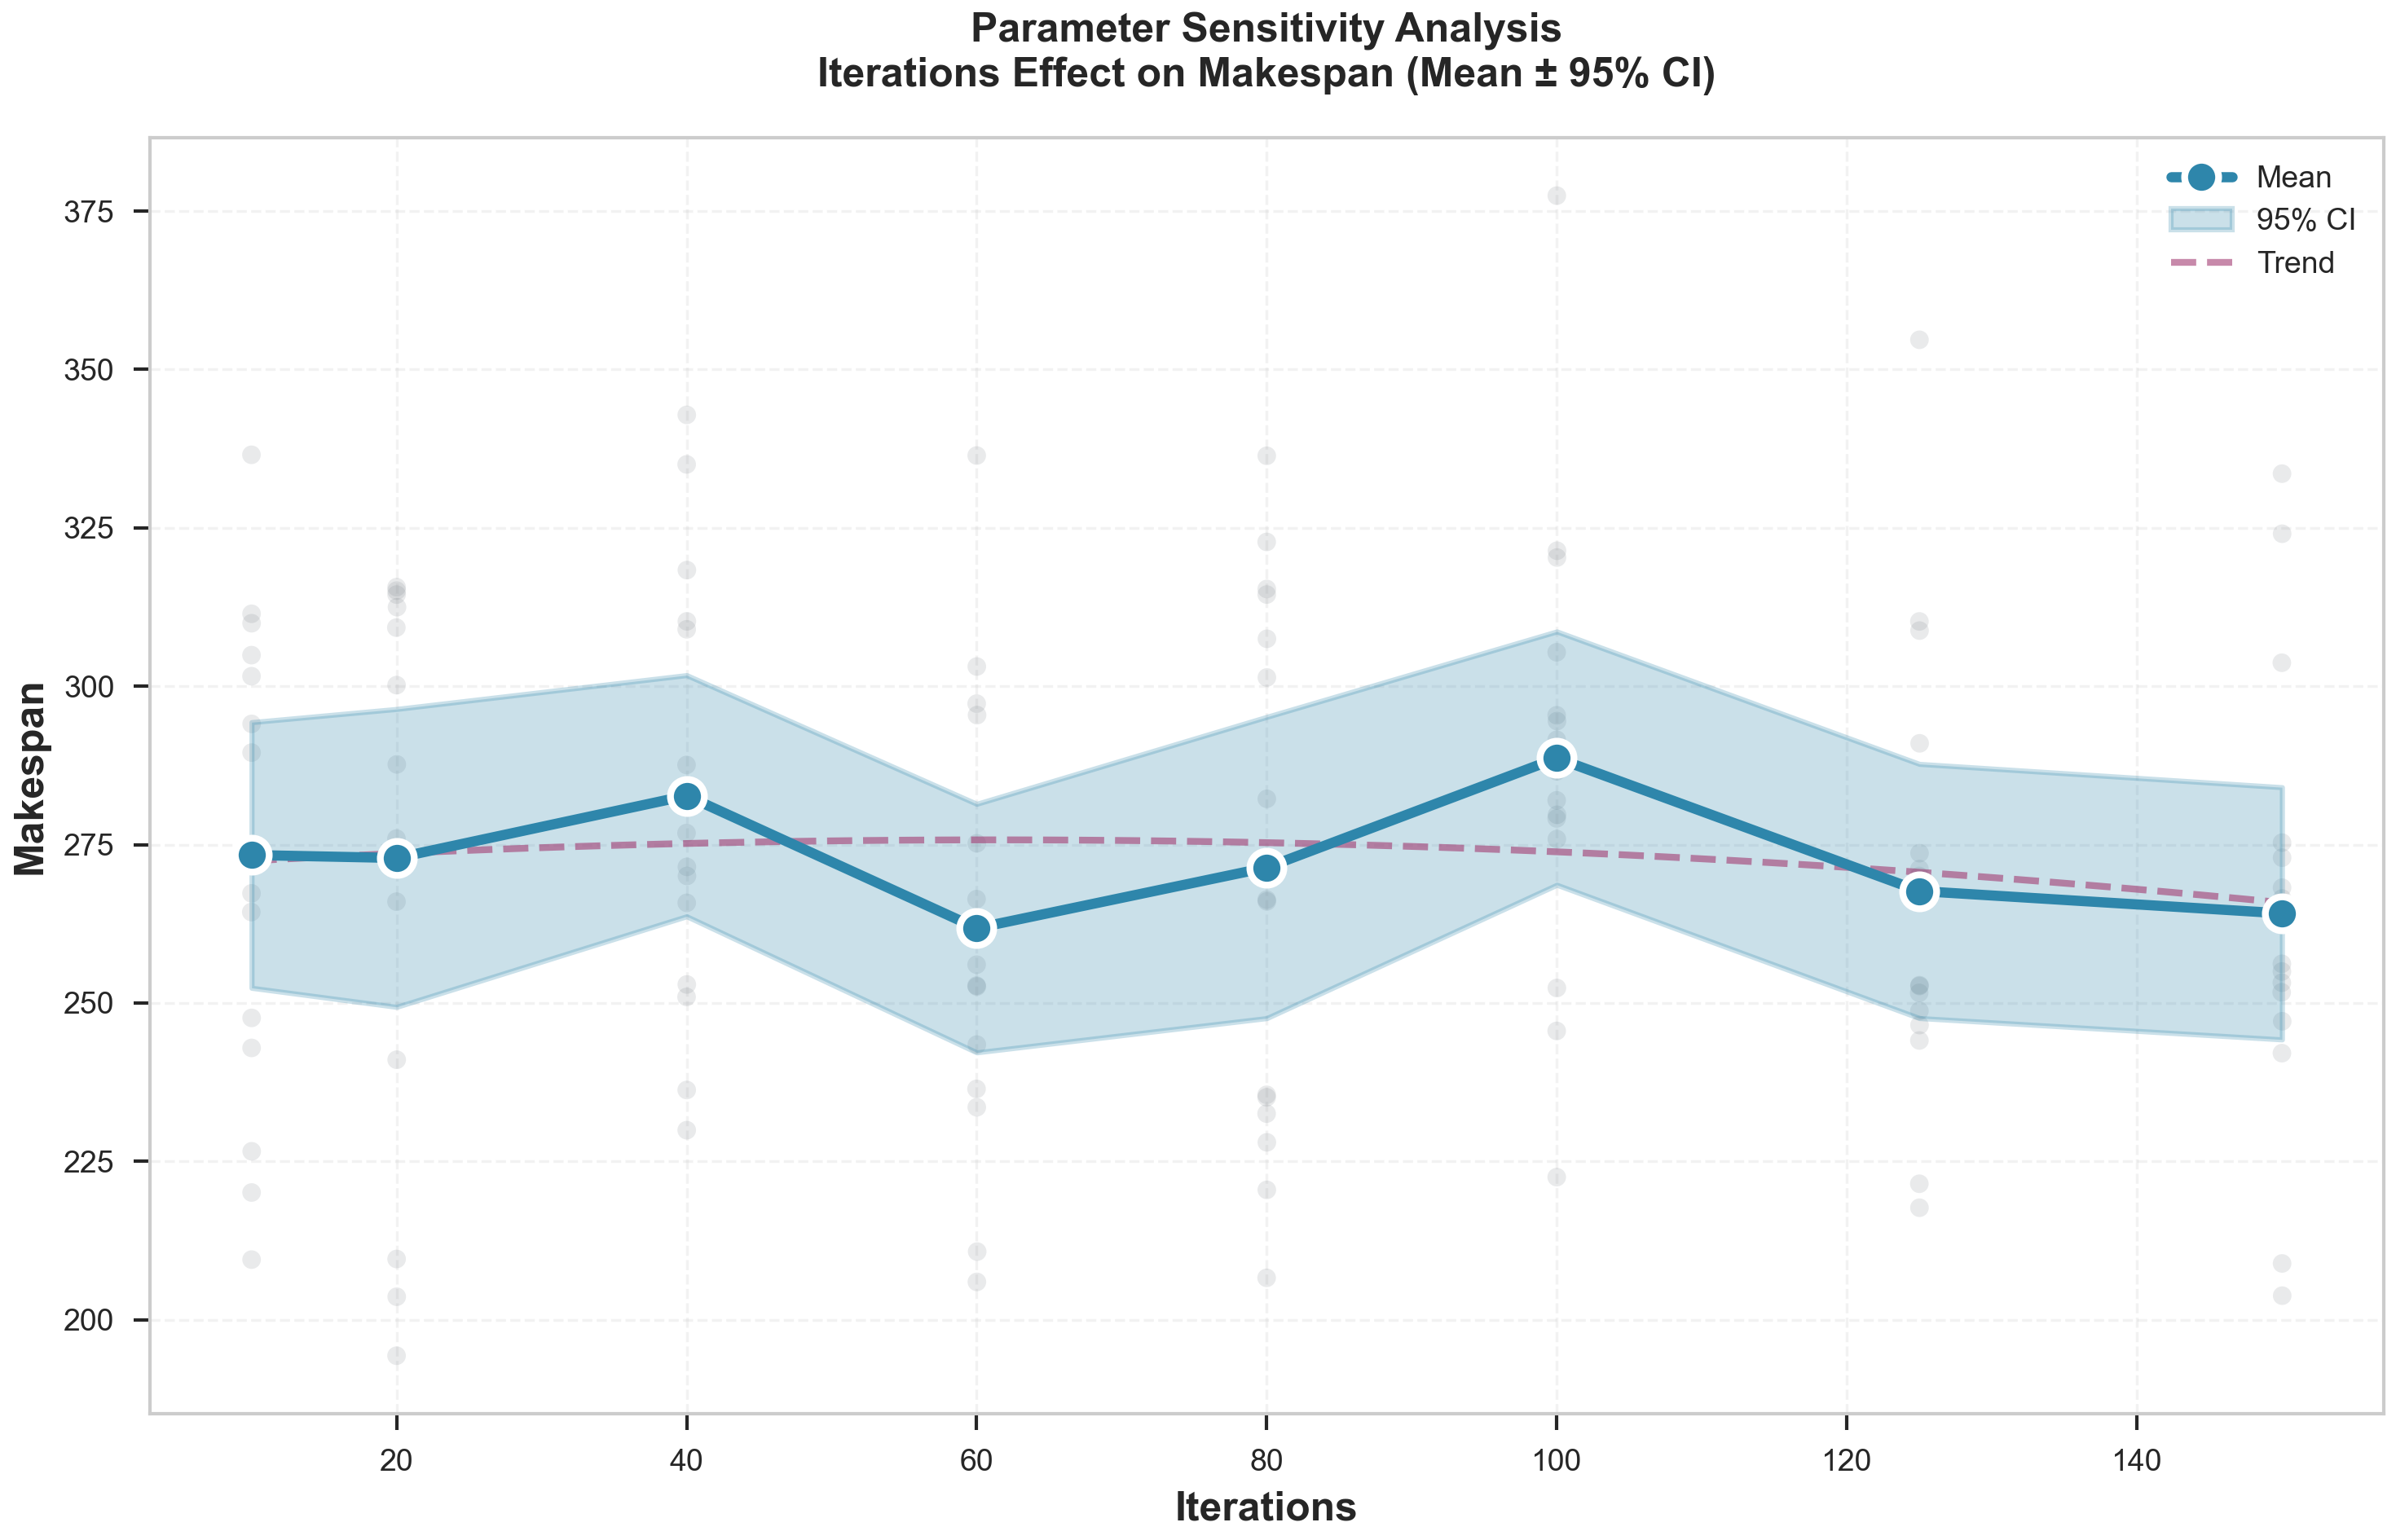
\includegraphics[width=0.95\textwidth]{Images/Results/ParameterAnalysis/Iterations_Makespan.png}
    \caption{Iteration sensitivity}
    \label{fig:iter_ms}
\end{subfigure}
\caption{Parameter sensitivity analysis using makespan metric}
\label{fig:param_makespan}
\end{figure}

\textbf{Alpha ($\alpha$):} We tried setting alpha parameter from 0.05 till 0.60 with gap of 0.05 between each simulation. Alpha exhibited moderate sensitivity to the scheduling performance of RDA. Makespan values for alpha ranged from 239 ms at $\alpha = 0.1$ to 273 ms at $\alpha = 0.45$. The unusual dip of Makespan at $\alpha = 0.1$ is although theoretically an optimal value but it resulted in reduced overall solution quality. We took the $\alpha = 0.35$ as the baseline as it lies within the optimal region where makespan variance is not high.

\textbf{Beta ($\beta$):} The inter harem mating parameter $\beta$ was again simulated with value ranging from 0.05 to 0.60. It demonstrated similar behavior to $\alpha$, with makespan ranging from 242 ms to 281 ms. Optimal performance was at around $\beta = 0.25-0.35$. Hence, we choose the beta to be as 0.30 which is within the optimal range. Beta parameter seemed to more sensitive than alpha in terms of scheduling outcomes.

\textbf{Gamma ($\gamma$):} The commander fraction parameter $\gamma$ was simulated in between the range of 0.10 to 0.60 which exhibited makespan values between 263 ms and 275 ms. Gamma was the least sensitive among the parameters. It represented a flat line and overlapping confidence intervals. A broad range of value for gamma (0.10-0.25 and 0.35-.40) produced equivalent results. The selected value for gamma experimentally is chosen to be 0.45 as it provides balanced performance with minimal risk of performance degradation from parameter variation.

Overall, the parameter sensitivity analysis supports the RDA configuration specified in Table~\ref{tab:algo_params} ($\alpha = 0.35$, $\beta = 0.30$, $\gamma = 0.45$, iterations = 100) that it represents a globally robust choice that maintains stable performance across diverse workload scenarios and parameter variation ranges.

\subsection{Scalability Analysis}\label{subsec6.5}

we evaluated RDA's performance with varying infrastructure and workload scales in cloud environments spanning from small scale configurations (3 hosts, 10 VMs, 100 cloudlets) to large scale configurations (20 hosts, 50 VMs, 2,000 cloudlets).

\begin{figure}[htbp]
    \centering
    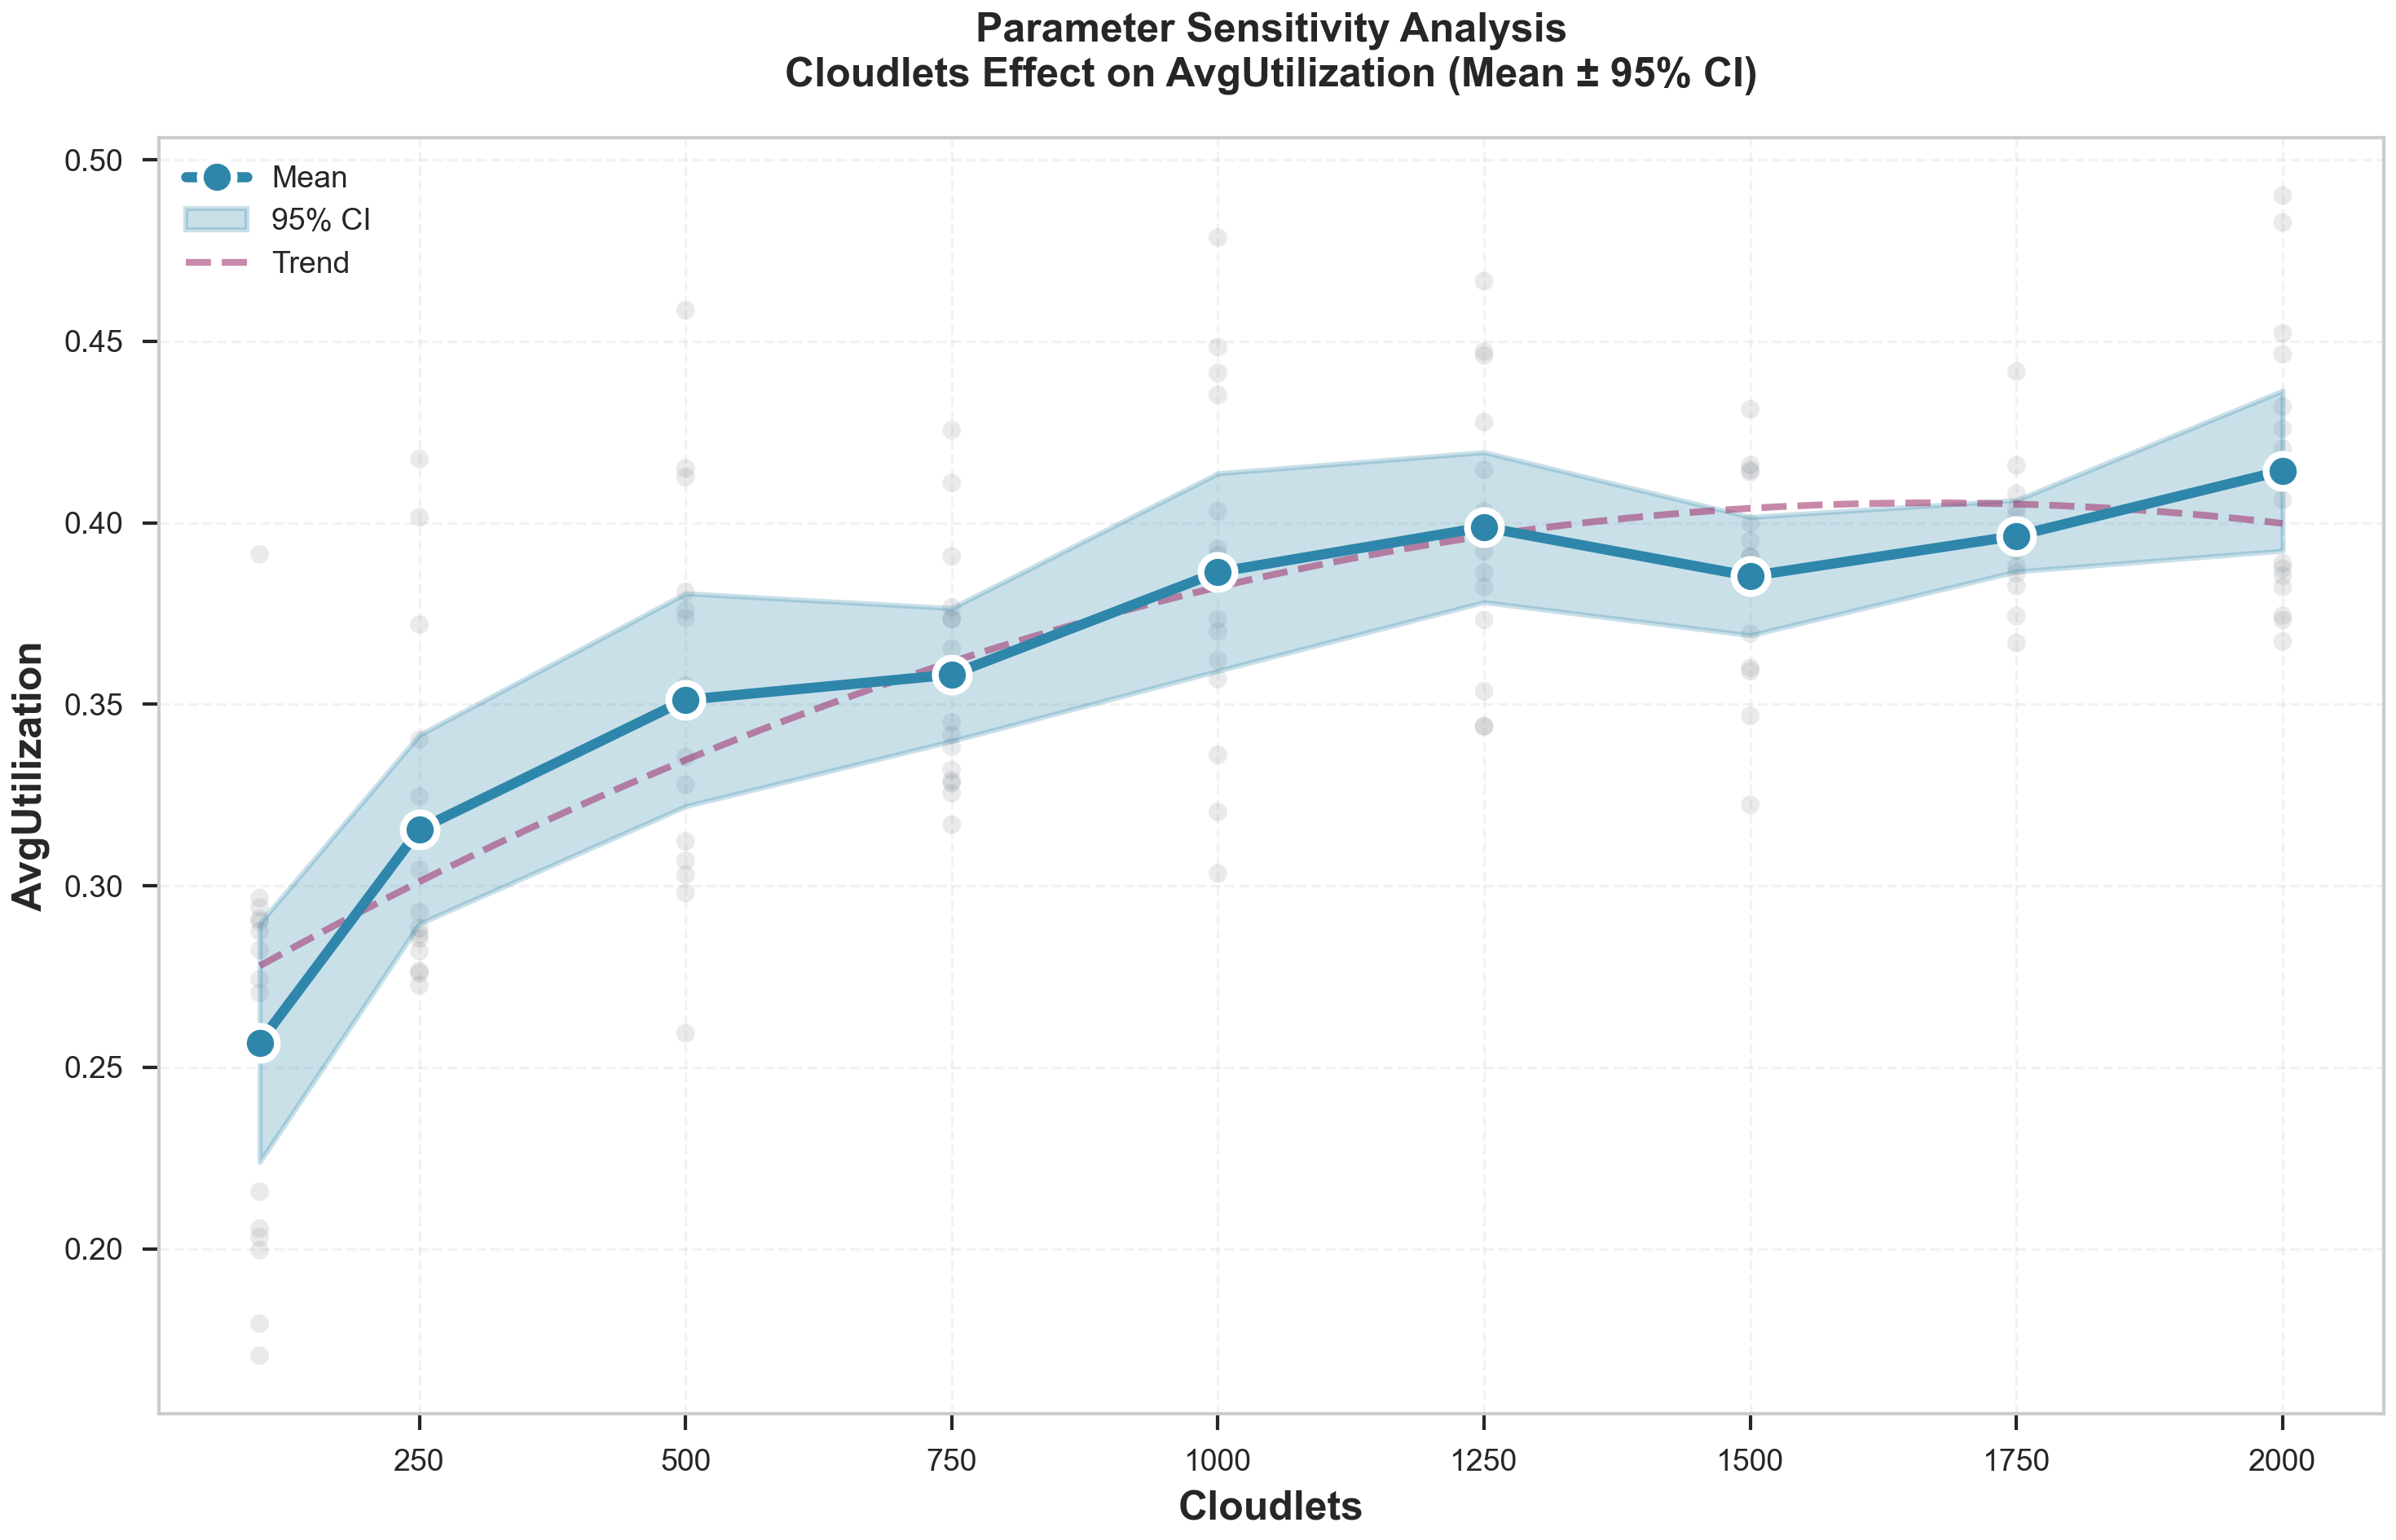
\includegraphics[width=\linewidth]{Images/Results/Cloudlets_AvgUtilization.png}
    \caption{Resource utilization under increasing cloudlet workloads}
    \label{fig:cloudlets_avgUtil}
\end{figure}

\textbf{Makespan and Response Time:} The RDA model demonstrates a linear makespan and response time scaling with respect to workload dicussed in Section \ref{subsec6.1}, \ref{subsec6.2}. This pattern for both metrics is consistent and supports that the RDA model can maintain effective solution efficiency even if workload increases, without visible performance degradation in comparison to other naive or inefficient scheduling approaches.

\textbf{Resource Utilization:} Fig.~\ref{fig:cloudlets_avgUtil} is the utilization Vs Cloudlet analysis for RDA model which shows efficient workload distribution across heterogeneous virtual machines. Analysis on the plot suggests mean virtual machine utilization from 0.26 at 100 cloudlets to 0.42 at 2,000 cloudlets, representing a 61.5\% improvement in resource utilization efficiency. It indicates that as workload increase, RDA model's solution exploits available VM capacity through better cloudlet to VM matching.

\textbf{Scalability Summary:} The observed linear scaling behavior, combined with high resource utilization even at high load tells that the RDA based scheduling is able to maintain stable optimized behavior as infrastructure and workload scale increases. These characteristics substantiate the algorithm's suitability for cloud deployments with dynamic, varying workload characteristics at scale.

\subsection{Statistical Validation}\label{subsec6.6}

To exclude the possibility that performance differences arose from random variation, multiple independent simulation runs (n=30 per algorithm workload combination) were conducted. Analysis of the results were performed using both parametric (t-test) and non-parametric (Wilcoxon rank-sum) statistical tests at a significance level of $\alpha_{\text{stat}} = 0.05$.

The t-test statistic is formulated as Eq. (\ref{eq:ttest}).

\begin{equation}\label{eq:ttest}
t = \frac{\bar{x}_1 - \bar{x}_2}{\sqrt{\frac{s_1^2}{n_1} + \frac{s_2^2}{n_2}}}
\end{equation}

where $\bar{x}_1$ and $\bar{x}_2$ represent mean performance metrics for compared algorithms, $s_1^2$ and $s_2^2$ denote sample variances, and $n_1$ and $n_2$ represent sample sizes.

\begin{table*}[htbp]
\centering
\caption{Statistical comparison of scheduling algorithms}
\label{tab:statistical_tests}
\resizebox{\textwidth}{!}{
    \begin{tabular}{lccc}
        \toprule
        \textbf{Comparison} & \textbf{T-Test p-value} & \textbf{Wilcoxon p-value} & \textbf{Effect Size} \\
        \midrule
        RDA vs PSO & $2.99 \times 10^{-7}$ & $2.37 \times 10^{-5}$ & Large \\
        RDA vs WOA & $1.97 \times 10^{-8}$ & $1.42 \times 10^{-6}$ & Large \\
        RDA vs GA & $4.99 \times 10^{-8}$ & $8.01 \times 10^{-8}$ & Large \\
        RDA vs GWO & $9.60 \times 10^{-9}$ & $2.05 \times 10^{-7}$ & Large \\
        PSO vs WOA & 0.3571 & 0.2894 & Small \\
        PSO vs GA & 0.0340 & 0.0549 & Medium \\
        PSO vs GWO & 0.0677 & 0.0879 & Small \\
        WOA vs GA & 0.1550 & 0.2449 & Small \\
        WOA vs GWO & 0.3123 & 0.3085 & Small \\
        GA vs GWO & 0.6076 & 0.8236 & Negligible \\
        \bottomrule
    \end{tabular}
}
\end{table*}


\begin{figure*}[htbp]
\centering
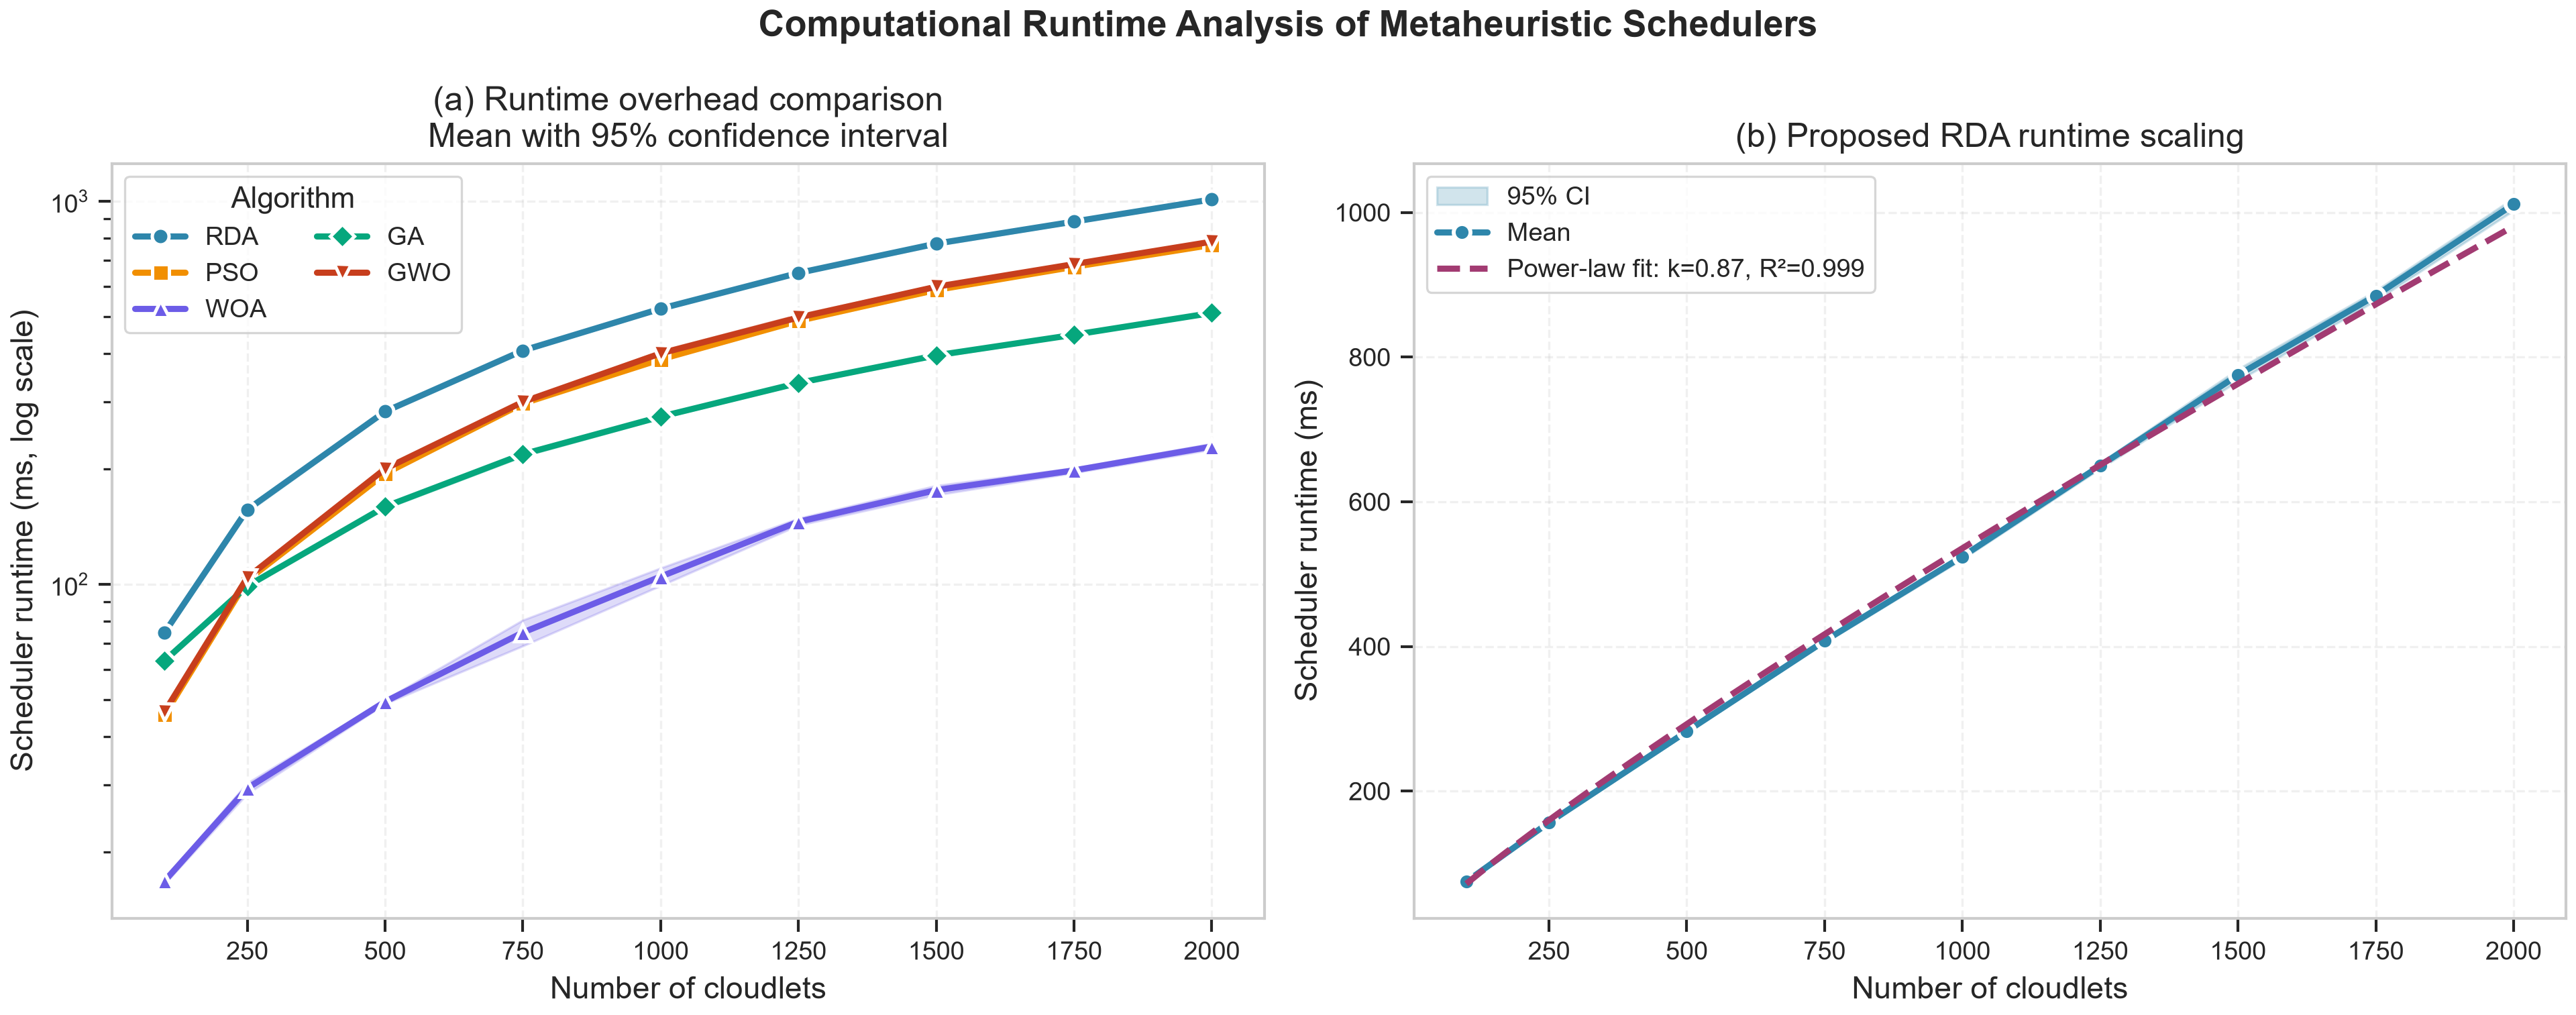
\includegraphics[width=\textwidth]{runtime_scalability.png}
\caption{Computational runtime analysis of the evaluated metaheuristic
schedulers: (a) mean wall clock scheduling runtime under increasing cloudlet
workloads on a logarithmic scale; (b) empirical runtime scaling of the
proposed RDA. Error bars represent 95\% confidence intervals across
independent runs.}
\label{fig:runtime_scalability}
\end{figure*}


\subsection{Runtime Overhead Analysis}
\label{subsec:runtime_overhead}

Figure~\ref{fig:runtime_scalability} presents the wall clock scheduling
runtime of the proposed RDA and the competing metaheuristic algorithms under
increasing cloudlet workloads. This metric measures the computational time
required by an algorithm to generate a cloudlet to VM mapping. The reported values are mean scheduler runtimes, with 95\% confidence intervals obtained from the independent experimental runs.

As shown in Fig.~\ref{fig:runtime_scalability}(a), the runtime of all
algorithms increased as the workload grew from 100 to 2,000 cloudlets.
This increase is expected because larger workloads require each candidate
schedule to evaluate a greater number of cloudlet-to-VM assignments in every
iteration. RDA incurred the highest runtime across the tested
workloads, increasing from approximately 67 ms at 100 cloudlets to
approximately 1,010 ms at 2,000 cloudlets.

The additional overhead of RDA is attributable to its population update and
selection operations, including roaring, fighting, harem formation, and
mating, in addition to repeated fitness evaluations. This overhead should be
interpreted alongside the improvements in makespan, response time and resource
utilization reported in the preceding sections.

Figure~\ref{fig:runtime_scalability}(b) further shows that the runtime of
RDA followed a smooth near-linear scaling pattern over the evaluated workload
range. The fitted power-law exponent of \(0.87\) with \(R^2=0.999\) indicates
a strong empirical relationship between cloudlet count and scheduler
runtime. This empirical fit is consistent with the expected polynomial
computational cost of population based RDA for fixed population size and
iteration count but it does not replace the worst case theoretical complexity
analysis presented in Section~\ref{subsec:complexity_analysis}.


\textbf{Results and Interpretation:} Comparison of all algorithms is stated pairwise. Comparisons involving RDA obtained p-values substantially below the significance threshold ($p < 0.001$ for both t-tests and Wilcoxon tests), indicating statistically significant performance differences. Specifically: RDA versus PSO yielded t-test p-value $2.99 \times 10^{-7}$ with Wilcoxon p-value $2.37 \times 10^{-5}$ (large effect size); RDA versus WOA produced p-values of $1.97 \times 10^{-8}$ and $1.42 \times 10^{-6}$ respectively; RDA versus GA achieved $4.99 \times 10^{-8}$ and $8.01 \times 10^{-8}$; and RDA versus GWO demonstrated $9.60 \times 10^{-9}$ and $2.05 \times 10^{-7}$.

Large effect sizes (Cohen's $d > 0.8$) in comparisons involving RDA indicate that observed improvements are  statistically significant and represent practically meaningful performance gains.

In contrast, comparisons among non-RDA algorithms (PSO vs. WOA: p = 0.3571; PSO vs. GA: p = 0.0340; WOA vs. GWO: p = 0.3123) revealed relatively similar scheduling behavior with smaller effect sizes.

In summary, the statistical analysis supports the proposed RDA based scheduling in achieving statistically significant performance improvements over established metaheuristic algorithms.

\FloatBarrier
\section{Conclusion and Future Work}\label{sec7}

This study proposed an RDA based task scheduling approach for load balancing in cloud computing environments. RDA was compared against four other metaheuristic algorithms: GA, PSO, GWO and WOA. Performance was benchmarked across four criteria: makespan, response time, resource utilization and cost under varying workloads and cloud configurations using CloudSim Plus. Experimental and statistical results illustrate RDA consistently outperformed competing algorithms across all the evaluation metrics. This performance is attributed to its effective balance between exploration and exploitation via its evolutionary behavior. These findings establish RDA as a competitive and scalable candidate for solving NP hard  combinatorial problems, particularly load balancing in cloud computing.

Nevertheless, several limitations of this study should be acknowledged. The proposed model primarily evaluates cloud scheduling performance using makespan, response time, resource utilization, and execution cost. Although explicit SLA violation modeling is not incorporated, response time and its statistical consistency provide an indication of service level performance. Energy consumption, fault tolerance, security, and carbon footprint are not explicitly modeled as optimization objectives in the current framework, and would require additional system level models and constraints beyond the scope of the present study. The scheduling objectives are also combined via a weighted sum formulation rather than a Pareto based approach, and the model assumes independent cloudlets within a static cloud environment, without accounting for inter task dependencies, dynamic workload arrivals, or VM failure and recovery events.

These limitations point to several directions for future work: extending the framework toward energy-aware, SLA-aware, fault tolerant, secure, and environmentally sustainable cloud scheduling; adopting Pareto based multi objective optimization to explore the full trade off surface among objectives; incorporating workflow aware scheduling that accounts for inter task dependencies and additional fairness metrics such as Jain's Fairness Index \cite{Jain_fairness_index}; and developing hybrid metaheuristic algorithms and adaptive scheduling strategies for dynamic cloud conditions, including VM failure and recovery handling.

\textbf{Funding} The authors declare that no funds, grants, or other support were received during the preparation of this manuscript.

\textbf{Data Availability} We used the open-source Java-based CloudSim framework to simulate the cloud environment. The data used in the current study are available from the corresponding author upon reasonable request.

\textbf{Declarations}

\textbf{Conflict of Interest} The authors declare that there are no conflicts of interest regarding the publication of this paper.

\textbf{Ethical Approval} This manuscript represents the authors’ original research and has not been published or submitted elsewhere. All co-authors have made significant intellectual contributions, are fully acknowledged, and collectively assume responsibility for the content. The work appropriately cites all relevant sources, ensuring transparency and academic integrity.

\textbf{Informed Consent} All authors have given informed consent for the publication of this manuscript.

\bibliography{sn-bibliography}

\end{document}
